% ------------------------------------------
%  MASTER THESIS DISSERTATION
% ------------------------------------------
% Author:
%
% Advisors:
%
% ------------------------------------------
\documentclass[10pt,twoside,openright,a4paper]{report}
\usepackage[utf8]{inputenc}
% Set document margins to 1in in all sides
\usepackage[margin=2.5cm]{geometry}
% Line spacing package
\usepackage{graphicx, helvet, hyperref, setspace}
\usepackage[portuguese,english]{babel}
\usepackage[nomain, acronym, toc]{glossaries}
% Extra stuff file
% This file is included before begin{document} environment
% Use this to include extra packages and define your own commands
% This way, you can easily grab a most recent version
% of dissertation.tex file from the original repo
\usepackage[explicit]{titlesec}
\usepackage[svgnames]{xcolor}
\usepackage{calc}
\definecolor{ChapNumColor}{gray}{0.90}
\definecolor{gainsboro}{rgb}{0.86, 0.86, 0.86}
\definecolor{lavender}{rgb}{0.9, 0.9, 0.98}
\definecolor{lavendergray}{rgb}{0.77, 0.76, 0.82}
\colorlet{chapnumcolor}{lavendergray}
\newcommand*{\chapnumfont}{%
  \usefont{T1}{jkp}{l}{l}%
  \fontsize{160}{180}%
  \selectfont%
}
\newcommand*{\chaptitlefont}{%
  \usefont{T1}{phv}{l}{l}%
  \fontsize{24}{24}%
  \selectfont%
}

\titleformat{name=\chapter}
{\normalfont\huge\bfseries}
{\filleft\parbox{0.10\textwidth}{\filleft\chapnumfont\color{chapnumcolor} \vspace{-0.7ex}\thechapter}\qquad}
{0pt}
{\filleft\llap{\parbox{\textwidth}{\filleft\chaptitlefont #1}}}

%\titlespacing*{\chapter}{10pt}{10pt}{10pt}
\newcommand*{\myfont}{\fontfamily{put}\selectfont}

% Built the glossary when the main file is built.
\makeglossaries
% Set main font to Arial
\renewcommand{\familydefault}{\sfdefault}
% Define keywords macro
\providecommand{\keywords}[1]{\textbf{Keywords:} #1}
% Define "palavras-chave" macro
\providecommand{\palavrasChave}[1]{\textbf{Palavras-Chave:} #1}
% Define the NewPage macro
\newcommand*\NewPage{\newpage\null\thispagestyle{empty}\cleardoublepage}
% Abstract-en page numbering
\newcommand {\abstractEnglishPageNumber} {\thispagestyle{plain}\setcounter{page}{\abstractEnglishPage}}
% Abstract-pt page numbering
\newcommand {\abstractPortuguesePageNumber} {\thispagestyle{plain}\setcounter{page}{\abstractPortuguesePage}}
% Section numbering depth
\setcounter{secnumdepth}{3}
% Table of contents depth
\setcounter{tocdepth}{3}
% Set line spacing to 1.5cm
\onehalfspacing
% Page numbering
\pagestyle{plain}

% Glossary-File
% Glossary Definition

\newglossaryentry{MSc}{name={MSc}, description={Masters degree in the area of Science.}}

% Acronym-File
% Acronym Definition

\newacronym{cad}{CAD}{computer-aided design}
\newacronym{gui}{GUI}{graphical user interface}
\newacronym{gd}{GD}{generative design}
\newacronym{ui}{UI}{user interface}
\newacronym{ast}{AST}{abstract syntax tree}
\newacronym{repl}{REPL}{read-eval-print loop}
\newacronym{bim}{BIM}{building information modeling}
\newacronym{jvm}{JVM}{Java virtual machine}
\newacronym{api}{API}{application programming interface}
\newacronym{gs}{GS}{General-purpose system}
\newacronym{ts}{TS}{Teaching system}
\newacronym{es}{ES}{Empowering system}
\newacronym{ocr}{OCR}{optical character recognition}
\newacronym{ide}{IDE}{Integrated Development Environment}

% ------------------------------------------
% MASTER THESIS DISSERTATION
% ------------------------------------------

\begin{document}
\pagenumbering{gobble}% Remove page numbers (and reset to 1)
\clearpage
\thispagestyle{empty}
%!TEX root = ./dissertation.tex

% Dissertation basic information
\newcommand {\Title} {An Enhanced Programming Environment for Generative Design}
%\newcommand {\Subtitle} {.}
\newcommand {\StudentName} {Guilherme Ferreira}
\newcommand {\DegreeName} {Information Systems and Computer Engineering}
\newcommand {\Supervisors} {{\large Prof. Dr. António Paulo Teles de Menezes Correia Leitão}}

% Include or not include acknowledgments
\def \includeAcknowledgments{1}

% Include or not include glossary
\def \includeGlossary{0}

% Examination Committee
\newcommand {\Advisor} {{\large Prof. Dr. António Paulo Teles de Menezes Correia Leitão}}
%\newcommand {\CoAdvisor} {{\large Prof./Dr. Co Advisor}}

% After the thesis defense
\newcommand {\CommitteeMembers} {
{\large Prof. Dr. Lorem Ipsum}}
\newcommand {\Chairperson} {{\large Prof. Dr. Lorem Ipsum}}

% Is final version (will include Committee Members information)
\def \IsFinalVersion{0}

% Date
\newcommand {\Month} {May}
\newcommand {\Year} {2016}

% Acknowledgments page number
\def \acknowledgmentsPage{1}

% Abstract-en page numbering
\def \abstractEnglishPage{3}

% Abstract-pt page number
\def \abstractPortuguesePage{5}

% You had a co-advisor:
\def \HasCoAdvisor{0}

% Logo Spacing Variables
\def \finalLogoSpacing{1.0cm}
\def \draftLogoSpacing{1.0cm}

% Logo home Variables
\def \logoHomeSpacing{0.5cm}

% Advisors Spacing Variables
\def \finalAdvisorsSpacing{1.5cm}
\def \draftAdvisorsSpacing{5.5cm}

% Date Spacing Variable
\def \dateSpacing{2.0cm}

% You can define your own variables here
\def \initialSpace{1.0cm}


	
%!TEX root = ./dissertation.tex

% ---------------------------------------------------------
%   MASTER THESIS DISSERTATION COVER
% ---------------------------------------------------------
\begin{titlepage}
% ---------------------------------------------------------
%  INSTITUTION LOGO
% ---------------------------------------------------------

\includegraphics[width=5cm]{images/ist_logo}~\\
%
\if\IsFinalVersion 1
  \vspace*{\finalLogoSpacing}
\else
  \vspace*{\draftLogoSpacing}
\fi

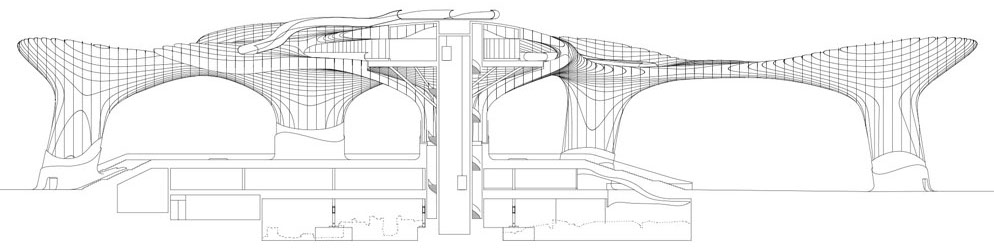
\includegraphics[width=\textwidth]{images/parasol}

\begin{center}
% ---------------------------------------------------------
%  MASTER THESIS DISSERTATION TITLE
% ---------------------------------------------------------
{\LARGE \textbf{\Title}}\\[2.0cm]
% ---------------------------------------------------------
%  MASTER THESIS DISSERTATION SUBTITLE
% ---------------------------------------------------------
%{\Large \Subtitle}\\[1.0cm]
% ---------------------------------------------------------
%  AUTHOR NAME (FULL)
% ---------------------------------------------------------
{\Large \textbf{\StudentName}}\\[1.0cm]
% ---------------------------------------------------------
%  DISSERTATION DEGREE
% -----------------------------------------------------------------
{\large Thesis to obtain the Master of Science Degree in}\\[0.5cm]
% -----------------------------------------------------------------
%  COURSE NAME
% -----------------------------------------------------------------
{\LARGE \textbf{\DegreeName}}\\[1.0cm]

% -----------------------------------------------------------------
%  ADVISORS NAME
% ---------------------------------------------------------
\begin{minipage}[t]{.24\textwidth}
  \center
  \begin{flushright}
    {\large Supervisor:~~}
  \end{flushright}
\end{minipage}%
\begin{minipage}[t]{.76\textwidth}
  \center
  \begin{flushleft}
    {\Supervisors}
  \end{flushleft}
\end{minipage}\\
%
\if\IsFinalVersion 1
  \vspace*{\finalAdvisorsSpacing}
\else
  \vspace*{\draftAdvisorsSpacing}
\fi
% ---------------------------------------------------------
%  JURI NAMES:
%  - PRESIDENT
%  - ADVISOR
%  - VOGALS
% ---------------------------------------------------------
%
\if\IsFinalVersion 1
%
\begin{minipage}[t]{1\textwidth}
  \center
  {\Large \textbf{Examination Committee}}\\[.25cm]
  {\large Chairperson: \Chairperson}\\
  {\large Supervisor: \Advisor}\\
  {\large Member of the Committee: \CommitteeMembers}
\end{minipage}\\[1.0cm]
%
\fi
%

\if\IsFinalVersion 1
 \vspace*{\dateSpacing}
\fi

% ---------------------------------------------------------
%  DATE (MONTH AND YEAR)
% ---------------------------------------------------------
{\Large \textbf{\Month\:\Year}}\\
\end{center}
\thispagestyle{empty}
\end{titlepage}


\NewPage

\pagenumbering{roman}

\if\includeAcknowledgments 1
%!TEX root = ../dissertation.tex

% Acknowledgments: This one is optional
\chapter*{Acknowledgments}
\thispagestyle{empty}
% Thanks to everyone and bla bla bla

\NewPage
\fi

%!TEX root = ../dissertation.tex

\begin{otherlanguage}{english}
% \begin{abstract}
% \thispagestyle{plain}
% Your abstract goes here.

% % Keywords
% \begin{flushleft}

% \keywords{my keywords}

% \end{flushleft}
% \end{abstract}

\chapter*{Abstract}
\thispagestyle{empty}

Increasingly more architects are moving from the traditional architectural processes and the classic forms of architectural coding to a modern area called Generative Design. \gls{gd} is the application of computational methods to design architectural structures or objects. In this area, designers write programs that when executed produce geometric models. This movement is clearly visible both in the academia, with current architecture curricula adopting programming courses, and in the industry, with design studios replacing traditional processes with computer applications.  However, for the most users, the transition from \gls{cad} applications to \gls{gd} methods can be quite significant. Therefore, it is important that \gls{gd} systems encourage users to learn, giving them the necessary support to evolve their knowledge and strategies. Unfortunately, the most used systems are not capable of responding to this need because they are old or obsolete, or they do not enforce any good principle of software engineering such as document code. To overcome this problem, this thesis proposes two programming tools for \gls{gd}  systems, namely (1) sketch-program correlation tool that allows architects to use sketches and combining them with code, and (2) immediate feedback tool that accelerates the effect of actions in the program output. We found that while the first tool turns program documentation in a less tiresome task, consequently minimizing the lack of documentation in the  \gls{gd} programs; the second tool enhances the program visualization, creating a new medium that helps people to design programs. This thesis uses Rosetta tool to implement and validate the proposed tools, clearly showing the advantages of this modern programming environment over the most used systems for \gls{gd}.

\begin{flushleft}
\keywords{immediate feedback; image correlation; DrRacket; Rosetta}
\end{flushleft}

\end{otherlanguage}
\NewPage
%!TEX root = ../dissertation.tex

\begin{otherlanguage}{portuguese}
% \begin{abstract}
% \thispagestyle{plain}
% O teu resumo aqui...

% % Keywords
% \begin{flushleft}

% \palavrasChave{as tuas palavras chave}

% \end{flushleft}

% \end{abstract}

\chapter*{Resumo}
\thispagestyle{empty}

Meu resumo...

\begin{flushleft}
\palavrasChave{palavras chave}
\end{flushleft}

\end{otherlanguage}

\NewPage

% Table of contents
\tableofcontents
% A new page is necessary only if table of contents has an odd number of pages
\NewPage

% List of tables
\addcontentsline{toc}{chapter}{\listtablename}
\listoftables
% A new page is necessary only if list of tables has an odd number of pages
\NewPage

% List of figures
\addcontentsline{toc}{chapter}{\listfigurename}
\listoffigures
% A new page is necessary only if list of figures has an odd number of pages
\NewPage

% List of acronyms
\printglossary[type=\acronymtype]

\pagenumbering{arabic}% Arabic page numbers (and reset to 1)

%!TEX root = ../dissertation.tex

% Entry point for chapters
% In this file you define the order
% in which the chapters are included

\setlength{\parindent}{2em}
% Configure the space between paragraphs
\setlength{\parskip}{1.0em}
%\setstretch{1.5} 

% Chapters
%!TEX root = ../dissertation.tex

\chapter{Introduction}
\label{chapter:introduction}
Your introduction here...\\

A demonstration of how to use acronyms and glossary:

A \gls{MSc} entry.

Second use: \gls{IST}.

Plurals: \glspl{MSc}.

A citation example \cite{nobody}

%!TEX root = ../dissertation.tex

\chapter{Background}
\label{chapter:generativeDesign}

In this chapter, I introduce the context and background for subsequent chapters. The first part addresses fundamentals concerning on teaching programming to novice students, and the relationship between programming and the related issues. The second part describes the typical components of software development environments used in Architecture, highlights the different types of available tools, and introduces the challenges of enabling programming on these environments.

\section{A Programming Framework}

Programming used to be taught mainly in computer engineering courses. In recent years the demand for programmers and student interest in programming have grown rapidly, and programming have become a subject increasingly important in several areas of study. Learning to program is hard however. Novice programmers suffer from wide range of difficulties and deficits. It is generally accepted that it takes about 10 years of experience to turn a novice into an expert programmer (Winslow, 1996).

Why programming is such a hard subject to learn? What resources and
processes are involved in creating or understanding a program? Since the 1970s there has been an interest in questions such as these, and in programming as a cognitive process. The literature relating to such topics is extensive, and it is divided into two main categories: those with a software engineering perspective, and those with a psychological/educational perspective.

Learning to program is usually addressed from a psychological/educational perspective, however our interest is in novices and in how the programming environment can provide adequate tools to support the initial development of individual programming skills. Early learning should of course include the basics of good software engineering practice such as comprehend the program structures, documenting the program, testing and debug among others.

Before propose any kind of feature it is first necessary to research what are the main challenges in this area. In fact programming is beyond coding, it involves knowledge about computer, programming language, programming tools and resources, and ideally theory and formal methods. As important as knowledge is the way knowledge is used and applied, also known as strategy. Writing a program involves also maintaining many different kinds of ‘mental model’ which is the way programmers comprehend its programs.

\begin{table}[!htbp]
\centering
\begin{tabular}{@{}lllll@{}}
\cmidrule(r){1-4}
 & \textbf{Design} & \textbf{Generation} & \textbf{Evaluation} &  \\ \cmidrule(r){1-4}
\textbf{Knowledge of} & \begin{tabular}[c]{@{}l@{}}planning methods,\\ algorithm design,\\ formal methods\end{tabular} & \begin{tabular}[c]{@{}l@{}}language, libraries,\\ environment / tools\end{tabular} & \begin{tabular}[c]{@{}l@{}}debugging tools\\ and methods\end{tabular} &  \\ \cmidrule(r){1-4}
\textbf{Strategies for} & \begin{tabular}[c]{@{}l@{}}planning,\\ problem solving,\\ designing algorithms\end{tabular} & \begin{tabular}[c]{@{}l@{}}implementing\\ algorithms, coding,\\ accessing knowledge\end{tabular} & \begin{tabular}[c]{@{}l@{}}testing, debugging,\\ tracking / tracing,\\ repair\end{tabular} &  \\ \cmidrule(r){1-4}
\textbf{Models of} & \begin{tabular}[c]{@{}l@{}}problem domain,\\ notional machine\end{tabular} & desired program & actual program &  \\ \cmidrule(r){1-4}
\end{tabular}
\caption{My caption}
\label{tab:framework}
\end{table}


The Table~\ref{tab:framework} (adapted from~\cite{robins2003learning}) proposes a programming framework that makes explicit the implied relationships between many of the issues found by novice programming. It highlights the relationship between the individual attributes (discussed above) with the program phases namely design, generation and evaluation. Undoubtedly the three phases are important, however the design phase is the most important because it is the basis of program understanding

Rist notes: There is considerable evidence in the empirical study of programming that the plan is the basic cognitive chunk used in program design and understanding.

\section{Coding in Architecture}

\section{Programming Languages \& Programming Environments}

%TEX root = ../dissertation.tex

\iffalse \bibliography{bibliography/dissertation} \fi


\chapter{Related Work}
\label{chapter:relatedWork}

In this chapter, I summarize related research on development environments and programming languages. Work presented here focuses on the programming tools used in different contexts and environments, whereas technical aspects and software architecture are separately discussed in Chapter x. Also, this chapter includes work on improvements to code intelligence features such as representation of code.

My work lies at the intersection of two main research areas: \gls{se} and \gls{gd}, consequently the related work present the recent advances in both of these areas.

\section{Programming System}
\label{sec:ps}
A \textit{programming system} has two fundamental parts: the \textit{programming language} that users should know in order to create a program, and the \textit{programming environment} that is used to write and test programs. Undoubtedly, both parts are equally important to build a program and understand it. However the boundaries between these parts can be blurred, for this reason the related work goes beyond programming environments including also programming languages and their design aspects. 

Based on prior surveys of novice programming environments~\citep{kelleher2005lowering}, in the following sections I divide the programming systems in three categories: (\ref{sec:gs}) general-purpose systems; proposed for building complex software, (\ref{sec:ts}) teaching systems; proposed to teach programming, and (\ref{sec:es}) empowering systems; proposed to build programs tailored to specific needs. In each category, we focus on the tools provided by the programming environment.
%%%
\section{General-purpose systems}
\label{sec:gs}

The systems in this category are built to support all, or at least a substantial part, of the software development process. To this end, these systems suggest an \gls{ide} that aims to support the entire development process by grouping in a single environment all necessary tools.

In this section we describe, in detail, two relevant \glspl{ide}: Eclipse~(open-source)~\citep{carlson2005eclipse} and LightTable (open-source)\footnote{\label{fnote:lt}\texttt{http://lighttable.com/}}. Other popular \glspl{ide} include NetBeans~(open-source)~\citep{boudreau2002netbeans}, Microsoft's Visual Studio~(commercial)~\citep{guckenheimer2006software}, or Apple's Xcode~(free but closed-source)\footnote{\texttt{https://developer.apple.com/xcode/}}. Some \glspl{ide} (eg., Visual Studio or Xcode) primarily target the environment and ecosystem of the manufacturer's own programming languages.  The following study use those \glspl{ide} for the sake of comparison, because they provide similar features to Eclipse or LightTable.

%%%%%%%%%%%%%%%%%%%%%%%%%%%%%%%%%%%%%%%%%%%%%%%%%%%%%%%%%%%%%%%%%%%%%%%%%%%%%%%%%%%%%%%%%%%%%%%%%%%%%%%%%
\subsection{Eclipse} 
\label{subsec:eclipse}
Eclipse~(Figure \ref{fig:eclipse}), a project initiated in 2001 and promoted by a consortium of industry leaders~\citep{carlson2005eclipse}, is a widely used open-source \gls{ide}. It is used mainly by Java developers, although it supports other programming languages such as C, C++ and JavaScript. As showed in~\citep{murphy2006java}, the commonly cited reasons for using Eclipse include rich Java development tools support and a \textit{plugin} architecture, the Eclipse Platform~\citep{DesRivieres2004}, that allows tight integration of third-party functionality.

The Eclipse platform~\citep{DesRivieres2004} has a common architecture among the \glspl{ide} presented in this category. This architecture is characterized by two main components, the \textit{plugin} which is the smallest unit of functionality that can be developed and delivered separately, and the platform runtime which will discover and connect the \textit{plugins} to the platform itself. As a result, the platform integrates several tools that are used in distinct phases of the software development process. Figure~\ref{fig:eclipse} shows the \gls{ide} opened in the Java perspective, suggesting a quick fix for the error.

\begin{figure}[!htbp]
%\vspace{-5pt}
  \centering
  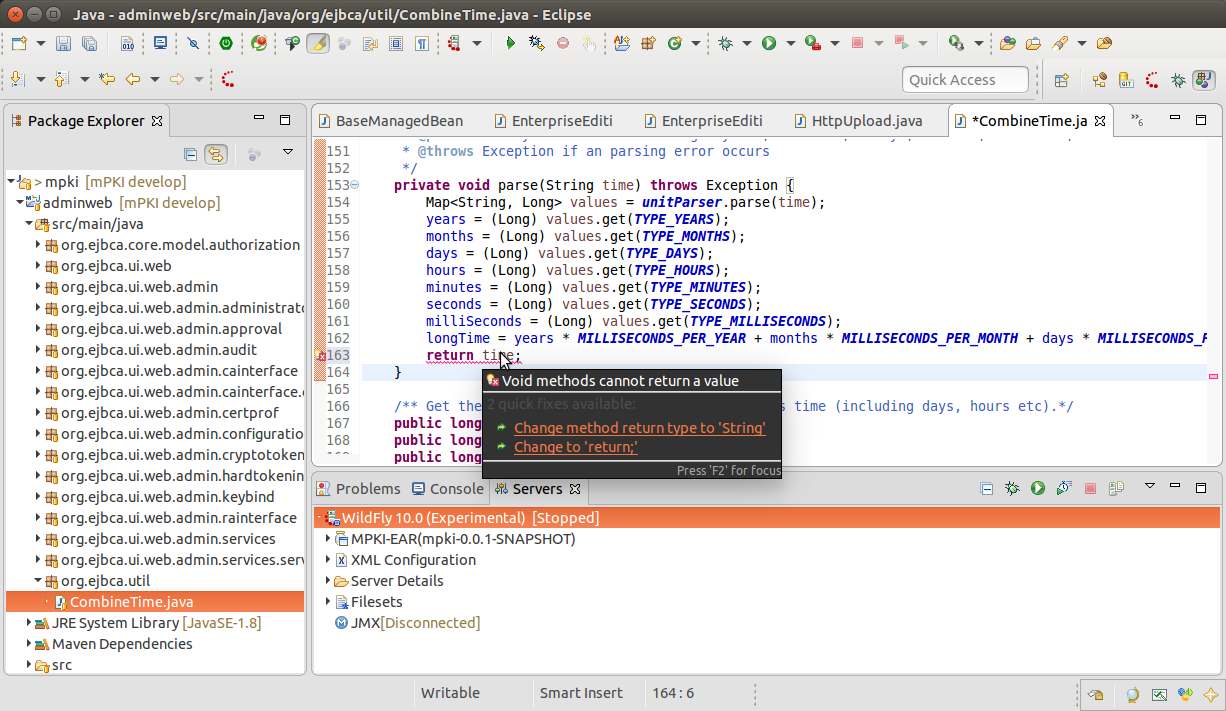
\includegraphics[width=1.0\textwidth]{images/eclipse-2}
    %\vspace{-15pt}
    \caption{Eclipse Integrated Development Environment showing Java perspective}
    %\vspace{-5pt}  
  \label{fig:eclipse}
\end{figure} 

Programming is a laborious task, even worse with verbose programming language such as Java. For example, while the developer is writing code he usually makes some errors, from lexical errors to semantic errors, that he will only detect after compiling the code. So, he needs to stop his main task to compile the code, and eventually debug it. This edit-compile-debug cycle is extremely unproductive and naturally undesired in an industry environment. 

To prevent this problem a common feature among \glspl{ide} is the instant feedback. This feature aims to anticipate the state of the current program by indicating eventual errors or mistakes made during development. To provide instant feedback Eclipse is constantly compiling the code in background, and giving immediate feedback for the developer in form of syntax highlighting, code completion suggestions, and indications of problems associated with various locations in a source file. 

In the literature a similar concept, known as \textit{liveness}~\citep{alpern1985defining}, referring to the ability to modify a running program. There are several levels of liveness and this kind of tool represent the first level~\citep{tanimoto2013perspective}. The tools in the first levels respond after a programmer action, while the tools at the last level not only run the program and respond immediately, but also predict the next programmer action. Having those tools in a \gls{ide} would be the ideal, however it is far from the reality of nowadays \glspl{ide} tools. 

Before to idealize any new features is important to highlight the drawbacks of the existent ones. Eclipse as the other similar \glspl{ide} share some problems, as for instance:

\begin{itemize}
	\item They are incidentally complex. There is an immense amount of work to be done in those \glspl{ide} that is indirectly related to the real problem itself. For example, until the programmer gets a simple program to run, he needs to install and configure a set of necessary software, and he needs also to configure the development environment. This is a tiresome and time consuming task that adds an extra complexity into programming which is already a complex subject.

	\item Program execution is difficult to observe, such that the only way to see how the program executes is by a stepwise debugger. This forces the programmer to stop the program and look at a line in a single instant of time. Consequently, the programmer cannot see how his program is executing, nor how his changes affect its execution.
\end{itemize}

The complexity of install and configure an \gls{ide} negatively affects the programming language itself, because users are more interested in the capabilities of the language than the \gls{ide}. To overcome this problem, recent programming languages, such as Rust~\citep{matsakis2014rust}, propose an \gls{ide} on the web browser\footnote{\texttt{https://play.rust-lang.org/}}. So users can write programs and use the language without any previous configuration. However this web environment is suitable only for tutorials and small examples, otherwise to have full access to the language users must pay the price to install and configure the language and the \gls{ide}.

%%%%%%%%%%%%%%%%%%%%%%%%%%%%%%%%%%%%%%%%%%%%%%%%%%%%%%%%%%%%%%%%%%%%%%%%%%%%%%%%%%%%%%%%%%%%%%%%%%%%%%%%%
\subsection{LightTable}
\label{subsec:lighttable}
LightTable$^{\ref{fnote:lt}}$ is a successfully crowd-funded project that indicates that instant feedback attracts wide interest beyond the research community. This is further supported by Apple, who have recently integrated a feature called Playgrounds into the Xcode \gls{ide}. Playgrounds are enabled by Apple's new programming language Swift\footnote{\texttt{https://developer.apple.com/swift/}} and allow developers to edit code and immediately see the results of execution.

LightTable is based on Bret Victor ideas which in his influential work~\citep{inventingPrin,learnableProg} pointed out serious problems with the current environments and showed, using prototypes, how the environment can help to address those problems. LighTable is proposed to build web application and to support this process, it provides, at least, two useful features: (1) live execution feedback, that executes the program on every change showing the program flow, and (2) the organization of code in tables, enabling quick access to the program documentation.

\begin{figure}[!htbp]
%\vspace{-10pt}
  \centering
  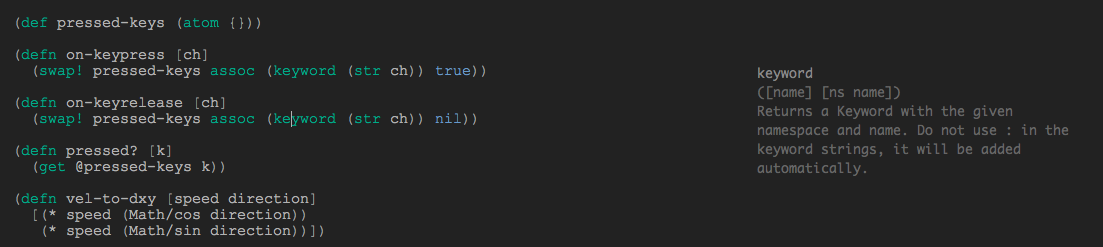
\includegraphics[width=1.0\textwidth]{images/lt2}
    %\vspace{-15pt}
    \caption{LighTable interactive development environment}
    %\vspace{-10pt}  
  \label{fig:lt}
\end{figure} 

LightTable was initially implemented in Clojure\footnote{\texttt{https://clojure.org/}} a general-purpose programming language dialect of Lisp that runs on top of \gls{jvm}. Progressively the code initially written in Clojure was rewritten in ClojureScript\footnote{\texttt{http://clojure.org/clojurescript}}, a script language that uses Clojure compiler which targets JavaScript. Due to its implementation, in LightTable adding a new \gls{ui} element into the programming environment or changing an existing one is doable in a short amount of time, contrary to other \glspl{ide}, such as Eclipse~\citep{carlson2005eclipse}, where an equivalent change requires considerable amounts of time. 

The program documentation in LightTable is quickly accessed by a lateral tab, where primitive functions of Clojure and ClojureScript can be consulted. This documentation is a textual description of the function parameters, the type of return, and some usage suggestions. While looking at a program, it is helpful to have the documentation of strange primitives, such as the \texttt{keyword} function shown in Figure~\ref{fig:lt}, however non-primitive functions are still undocumented. 

\begin{wrapfigure}{r}{0.3\textwidth}
  %\vspace{-30pt}
  \begin{center}
    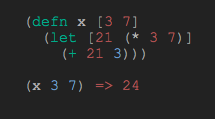
\includegraphics[width=0.3\textwidth]{images/eval-close}
  \end{center}
  %\vspace{-15pt}
 \caption{LightTable real-time debugger.}  
  %\vspace{-20pt}
    \label{fig:lt2}
\end{wrapfigure}

On the other hand, programmers are encouraged to understand new functions by seeing how the values of a function call flow through it. This feature is based on the old idea of Lisp environments: the \gls{repl} which is a prompt used to try out expressions of the language without having to run all the code. This approach goes further by using reflection mechanisms to trace the function call values and shows them filled in the function template (as shown in Figure~\ref{fig:lt2} the flow of values produced by calling \texttt{(x 3 7)}).

The real-timer debugger is an interactive way to debug the code and understand the program flow. Using this feature in an arbitrarily complex program (a program with more than 30 functions) is, however, worthless, because, all the programmer sees is a replica of his functions filled with numbers. It is a poor representation of flow which forces the programmer to spend as much effort with this feature as without it. For this reason, other systems, described in this report, represent the program flow using graphs which are more appropriate in some cases, for example, to show error occurrences in the source code.

Despite providing some tools which are state of the art, LightTable remains in an experimental phase. It has serious limitations to identify and clearly present the errors in the source code. This problem is, mainly, related with the Clojure compiler which loses significant \textit{metadata} between conversions. Consequently, programmers can spend more time and effort to find a bug using LighTable, than using the other \glspl{ide}, such as Eclipse.
%%%%%%%%%%%%%%%%%%%%%%%%%%%%%%%%%%%%%%%%%%%%%%%%%%%%%%%%%%%%%%%%%%%%%%%%%%%%%%%%%%%%%%%%%%%%%%%%%%%%%%%%%
\section{Teaching systems}
\label{sec:ts}
Unlike the previous systems, teaching systems are designed with the goal of helping people learning to program. Most of the systems in this category provide simple programming tools that expose the novice programmers some of the fundamental aspects of the programming process. After acquiring experience with a teaching system, students are expected to move to a more general-purpose environment. 

%%%%%%%%%%%%%%%%%%%%%%%%%%%%%%%%%%%%%%%%%%%%%%%%%%%%%%%%%%%%%%%%%%%%%%%%%%%%%%%%%%%%%%%%%%%%%%%%%%%%%%%%%
\subsection{LOGO} 
\label{subsec:logo}
LOGO~\citep{papert1980mindstorms} is a programming language and environment intended to allow children to explore a wide variety of topics such as physics and mathematics. The programming language is a dialect of Lisp, with much of the punctuation removed to make the syntax accessible to children, it uses a helpful metaphor which facilitates the introduction of programming concepts.

In Logo, the programmer draws pictures by directing the ``turtle'', an onscreen character which leaves a trail as it moves (see Figure~\ref{fig:turtle}). The turtle is a metaphor that helps learners to translate their experiences as a person into programming knowledge. That means, to figure out how to make the turtle perform an action, the programmer can ask how he would perform that action himself, as if he were the turtle.

\begin{wrapfigure}{r}{0.4\textwidth}
  %\vspace{-40pt}
  \begin{center}
    
\includegraphics[width=0.4\textwidth]{images/turtle}
  \end{center}
  %\vspace{-15pt}
 \caption{Directing the ``turtle''.}  
  %\vspace{-20pt}
    \label{fig:turtle}
\end{wrapfigure}

For example, to figure out how to draw a circle, a learner would walk around in circles for a bit, and quickly derive a ``circle procedure'' of taking a step forward, turning a bit, taking another step forward, turning a bit. After teaching it to himself, the learner can then teach it to the computer. 

LOGO has influenced several systems, and its principles show how a system can be designed around the way people think and learn.
%%%%%%%%%%%%%%%%%%%%%%%%%%%%%%%%%%%%%%%%%%%%%%%%%%%%%%%%%%%%%%%%%%%%%%%%%%%%%%%%%%%%%%%%%%%%%%%%%%%%%%%%%
\subsection{SmallTalk}
\label{subsec:smalltalk}
SmallTalk~\citep{Kay1993} is a programming language and environment to support children in the world of information. The designers of this system, wanted to create a programming language that had a simple model of execution and a programming methodology that could accommodate a wide variety of programming styles. SmallTalk was based around three ideas: (1) everything is an object, (2) objects have memory in the form of other objects, (3) and objects can communicate with each other through messages.

\begin{wrapfigure}{r}{0.5\textwidth}
%\vspace{-20pt}
  \centering
  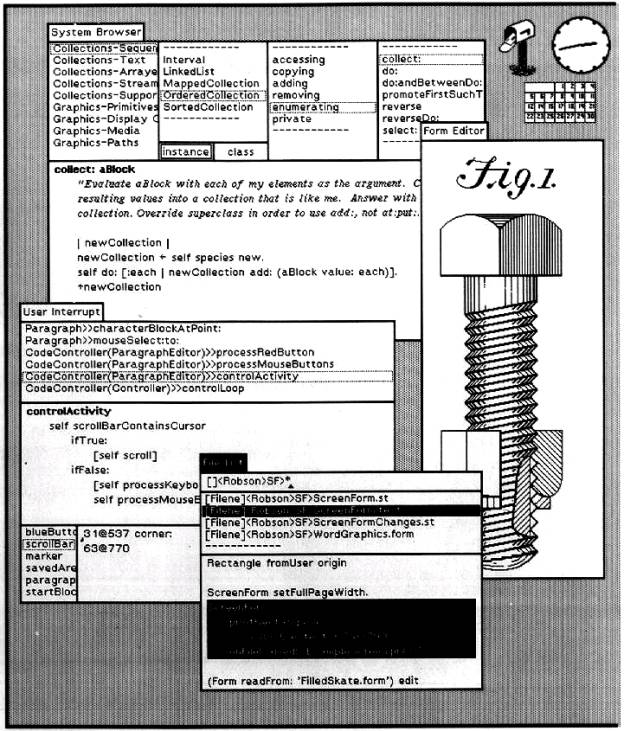
\includegraphics[width=0.5\textwidth]{images/smalltalk}
    %\vspace{-15pt}
    \caption{Smalltalk user interface.}
    \vspace{-20pt}  
  \label{fig:smalltalk}
\end{wrapfigure} 

Smalltalk programming environment was a successful achievement with relevant improvements on its successors. The system consisted of about 50 classes described in about 180 pages of source code~\citep{Kay1993}. This included all of the OS functions, files, printing and other Ethernet services, the window interface, editors, graphics and painting systems, as shown in Figure~\ref{fig:smalltalk}. 

In the Smalltalk programming language, the communication through messages has a strong resonant metaphor. To specify the behavior of an object, the programmer casts himself into the role of that object (to the extent of referring to the object as ``self'') and thinks of himself as carrying on a conversation with other objects. This is a strong metaphor, because role-playing and conversing are innate human facilities. 

In fact, SmallTalk features are, nowadays, a consistent reference for any programming system.
%%%%%%%%%%%%%%%%%%%%%%%%%%%%%%%%%%%%%%%%%%%%%%%%%%%%%%%%%%%%%%%%%%%%%%%%%%%%%%%%%%%%%%%%%%%%%%%%%%%%%%%%%
\subsection{Processing}
\label{subsec:processing}
Processing~\citep{Reas2006} is a programming language and environment designed to teach programming in a visual context. Processing has become popular among students, artists, designers, and architects, because it acts as a tool to get non-programmers started with programming through instant visual feedback.

The Processing programming language is built on top of Java, but it removes much of the verbosity of Java to make the syntax accessible to novices. The language provides simple access to external libraries, such as OpenGL, through single entry points, such as \texttt{setup} and \texttt{draw}. This allows novices to quickly prototype, learn fundamental concepts of programming, and, eventually, gain the basis to learn other programming languages.

The programming environment contains a simple text editor, a text console to present errors, and a run button. The run button compiles the Processing code and executes it. Despite in the default mode the result is presented in a 2D graphical window, the render can be configured to present the result in 3D or in other sophisticated methods using \textit{shaders} to recur directly to the graphic board.

Actually, with a few changes, the Processing code can be exported as an application for different platforms, such as Java, JavaScript, and Android. For example, to export a Processing program for JavaScript, it is only necessary to create a HTML page and include the Processing code as a script of this page. Then the Processing code will be automatically parsed and translated to JavaScript. To maintain the usual render capabilities of a Processing program it will use the HMTL5 canvas with WebGL.

The popularity of Processing is explained by the benefits of these features, besides of being a domain-specific language, however it has drawbacks that can discourage its use, such as the following:

\begin{itemize}
  \item \textit{Weak metaphor}. The Processing programming language, by contrast with the above systems, has none strong metaphors that allow the programmer to translate his experiences as a person into programming knowledge. 

  \item \textit{Poor decomposition}. Processing discourages the fundamental approach to solving a complex problem by breaking it into simpler problems, because drawing and input events are tied to single entry points. Thereby the behavior of submodules must be tangled across these global functions, making it difficult to achieve clean decomposition.

  \item \textit{Poor recomposition}. Processing discourages combining two programs. The programmer cannot just grab and use part of other programs, because variables must be renamed or manually encapsulated, and the \texttt{draw} and mouse functions must be woven together. Even worse, Processing has global modes which alter the meaning of the function arguments. For example, two Processing programs can specify its colors in different modes and each mode has its proper meaning of \texttt{fill} function arguments. Combining those programs will be almost impossible. 

  \item \textit{Weak readability}. The syntax of a Processing program represents a significant barrier for reading. For example, the function which draws an ellipse on screen is written as \texttt{ellipse(50,50,100,100)}. The reader must lookup or memorize the meaning of every single argument.

  \item \textit{Fragile environment}. The programming environment is fragile, because it does not attempt to solve any of the above issues related with the language and its implementation.
\end{itemize}

%%%%%%%%%%%%%%%%%%%%%%%%%%%%%%%%%%%%%%%%%%%%%%%%%%%%%%%%%%%%%%%%%%%%%%%%%%%%%%%%%%%%%%%%%%%%%%%%%%%%%%%%%
\subsection{Fluxus}
\label{subsec:fluxus}
Fluxus~\citep{griffiths2007fluxus}\footnote{\texttt{http://www.pawfal.org/fluxus/}} is a programming language and learning environment designed for rapid prototype using 3D graphics and sounds. This emphasis on rapid prototype and quick feedback makes Fluxus a tool for learning computer animation, graphics and programming. However, most users of Fluxus use it for \textit{livecoding}, which is the act of performing coding lively to an audience.

Fluxus is mainly written in C++ and it is statically linked to several shared libraries, specified at compile time. For instance, Fluxus uses \texttt{jack-audio}, \texttt{ode}, and \texttt{fftw} libraries to handle and synchronize the audio, \texttt{GLEW} to present graphics, and \texttt{racket3m} to embed the Racket run-time system into the application. In this way, Fluxus is an extension of Racket (a descendant of Scheme) with graphical commands.

Like Processing, Fluxus provides simple access to those libraries through single entry points, for instance \texttt{start-audio} connects an input audio to the application, \texttt{every-frame} registers a function called once per frame, and so on. However, as stated above, it is a barrier for decomposition since the behavior of submodules must be tangled across these global functions.

\begin{figure}[!htbp]
  \centering
  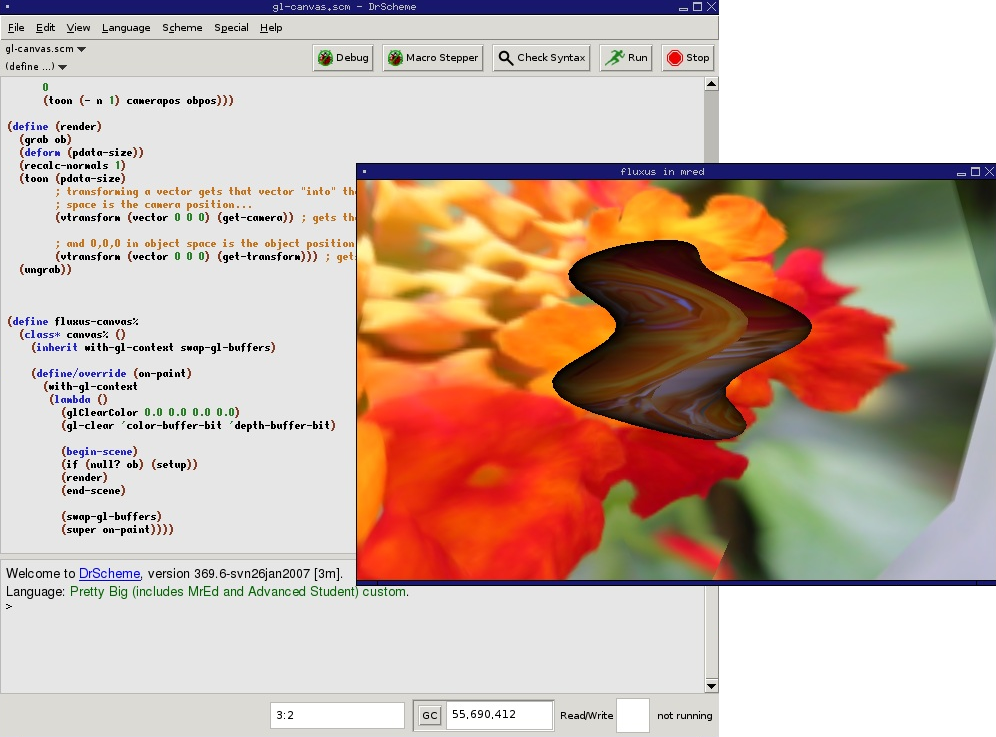
\includegraphics[width=.8\textwidth]{images/fluxus}
    \caption{Fluxus engine being used as DrRacket module}
  \label{fig:fluxus}
\end{figure} 

Fluxus has its own environment specifically tailored for \textit{livecoding}. It is composed by a OpenGL graphical window with a simple text editor. The programmer types his code in the editor and presses a shortcut key each time he wants to run the code. Fluxus evaluates the code through Racket run-time system and shows its result in the same graphical window that the code was written. This mechanism is valuable in an \textit{livecoding} environment, because the performer can be editing the code while the result of the previous computation is maintained in background. However, if the code has any error and the performer execute it, the previous computation disappears and the environment will not help to find it. This is a serious problem, specially for the Racket syntax.

Moreover, Fluxus shares with Processing similar drawbacks to those previously stated. However Fluxus can be used as a module of DrRacket (Figure~\ref{fig:fluxus})~\citep{findler2002drscheme} programming environment and, fortunately, in DrRacket the above problem and many others are solved.
%%%%%%%%%%%%%%%%%%%%%%%%%%%%%%%%%%%%%%%%%%%%%%%%%%%%%%%%%%%%%%%%%%%%%%%%%%%%%%%%%%%%%%%%%%%%%%%%%%%%%%%%%
\subsection{DrRacket}
\label{subsec:drracket}
DrRacket~\citep{findler2002drscheme} is a programming environment designed to support the Racket language. DrRacket is one of few programming environments which supports gradual learning in a more general language from the start. Consequently, it has been widely used in introductory programming courses in several universities around the world.

The usual scenario where DrRacket is used is to teach functional programming using Racket. To facilitate this process, DrRacket provides three tools. The first is a symbolic stepper. It models the execution of Racket programs as algebraic reductions, since Racket is implemented on top of lambda calculus. The second tool is a syntax checker. It annotates programs with font and color changes based on the syntactic structure of the program. It also permits students to explore the lexical structure of their programs graphically and to $\alpha$-rename identifiers. The third tool is a static debugger that infers which set of values an expression may produce and how values flow from place to place in the source text, and, upon demand, it explains the reason of errors by drawing value flow graphs over the program text.

Similar to Lisp environments, DrRacket provides a read-eval-print loop (\gls{repl}). This is a command prompt intended to quickly evaluate expressions and print their results. Especially in a learning environment, this feature makes an important connection between program execution and algebraic expression evaluation. However, the Lisp-style syntax obscures the effect of this feature. To overcome this limitation, DrRacket provides a \texttt{pretty-printer}. A module capable of printing algebraic expressions in a meaningful way, as well as other graphics elements supported by the text editor, such as images, snips, XML boxes, and so on.

More recently, DrRacket has included picture boxes for \gls{wysiwyg} layout of slide content that is otherwise created programmatically~\citep{findler2004slideshow}. This kind of presentation extensibility is in addition to recognizing standard Racket hygienic macros. There are several problems with this approach. First, there is no documented protocol for creating new kinds of boxes. Second, any program that uses boxes is stored as ascii-encoded binary and is difficult to edit outside of DrRacket. Last, the semantics of the boxes is driven off of the display itself, rather than the persistent store; therefore, in order to compile, interpret, or edit the program, a box-aware editor is required.

From the perspective of professional programmers DrRacket can be a potential target. It is useful for developing complex applications, including DrRacket itself. Moreover it is extensible by the same \gls{api} which the above tools implement. Through this \gls{api} it is also possible to extend the \gls{repl}, as in Pict3D\footnote{\texttt{https://github.com/ntoronto/pict3d}} (a 3D engine that integrates new graphical elements in the DrRacket environment). On the other hand, for supporting extensions, DrRacket's architecture has become increasingly complex. For instance, to make a simple change in an editor's element the programmer should be able to understand several modules, unrelated with the problem itself. This extra complexity is a negative impact when DrRacket is chosen as basis for new development tools.

Despite of the identified advantages, DrRacket has some barriers that may discourage the learner. For example, the Racket programming language is simple to teach, but its heavy syntax of s-expressions hinders the learner to read the program. Consequently, the learner can spend a huge mental effort to understand insignificant details of the language.
%%%%%%%%%%%%%%%%%%%%%%%%%%%%%%%%%%%%%%%%%%%%%%%%%%%%%%%%%%%%%%%%%%%%%%%%%%%%%%%%%%%%%%%%%%%%%%%%%%%%%%%%%
\subsection{PythonTutor}
\label{subsec:pythontutor}
PythonTutor~\citep{GuoSIGCSE2013} is a web-based program visualization tool, designed to explain how a piece of Python code executes. It has become popular among students from introductory Computer Science courses. Using this tool, teachers and students can write Python programs directly in the web browser and navigate step by step throughout its execution, seeing the run-time state of data structures.

PyhtonTutor has two main modules: the \textit{backend} which implements the tool core functionality, and the \textit{frontend} which presents the visualization of program's data structures. The \textit{backend} executes the input program under supervision of the standard Python debugger module (\texttt{bdb}) which stops execution after every executed line and records the program's run-time state. After execution terminates, the \textit{backend} encodes the program state in JSON format, serializing Python data types into native JSON types with extra \textit{metadata} tags and sends it to the \textit{frontend}. The frontend renders the objects using standard web technologies: HTML, CSS, and JavaScript. In this way, users can use the tool without installing any extensions or plugins.

A major concern in PythonTutor is security, because the PythonTutor's \textit{backend} executes untrusted Python code from the web. To prevent the execution of dangerous constructs such as {\tt eval}, {\tt exec} and {\tt file I/O}, PythonTutor implements sandboxing. Basically, it denies the use of most module imports, by parsing the user's code importing, a strict approach, but effective in this case.

The PythonTutor tool allows the programmer to follow the program execution over time, but he only sees a single point in time at any instant. There is no visual context at all. The entire program flow is represented by disconnected points in time. For example, the programmer who wants to understand a conditional algorithm, using this tool will not see the pattern of this algorithm neither understand it at a higher level.
%%%%%%%%%%%%%%%%%%%%%%%%%%%%%%%%%%%%%%%%%%%%%%%%%%%%%%%%%%%%%%%%%%%%%%%%%%%%%%%%%%%%%%%%%%%%%%%%%%%%%%%%%
\subsection{YinYang}
\label{subsec:yinyang}
YinYang~\citep{mcdirmid2013usable} is a prototype of a programming language and environment whose main feature is the live execution feedback. That means it combines editing and debugging, where updated debug results are conveniently visible while editing. YingYang addresses the above issue in two ways. First, just like the previous system, it allows programmers to see single points of execution directly within the code editor (probe; precede expressions with \texttt{@} operator). Second, it has a pane aside the editor which traces execution with entries that are navigable (trace; print-like statements). Basically, the trace is an enhanced display function which, combined with ``probes'', allows the state of previous executions to be restored. So, programmers can take in the entire program flow at a glance and navigate trough it using probes.

YingYang uses an incremental framework as basis of its programming model. This framework decomposes the program execution into a tree of nodes that can be re-executed independently on a code or input change. However, this decomposition cannot be performed transparently. It requires programmers to specify how the program will be decomposed. To perform this task one must deeply understand the granularity and modularity characteristics of the computations being performed by the program. Otherwise changes can sometimes have a huge impact on program re-execution time ($\sim$50ms). Consequently, live programming would actually reduce programmer productivity as programmers wait for slow feedback.

Although YinYang provides usable features for a learning environment, such as the live execution feedback, it does not have a suitable language for beginners. The language is merely experimental and to navigate through the program execution, programmers must include probes in the code. At the end of experimentation, the code is full of useless expressions.

%%%%%%%%%%%%%%%%%%%%%%%%%%%%%%%%%%%%%%%%%%%%%%%%%%%%%%%%%%%%%%%%%%%%%%%%%%%%%%%%%%%%%%%%%%%%%%%%%%%%%%%%%
\section{Empowering Systems}
\label{sec:es}
In this category of systems the most important aspect is to allow people to build programs tailored to their own needs. In this section, I describe how systems from two distinct areas are tailored to achieve their user's needs. 

First, I consider Architecture, where new programming languages and environments are being proposed to support the increasing use of \gls{gd}~\citep{mccormack2004generative}. \gls{gd} is a design method that uses algorithms to generate architectural models. Usually these models are rendered using a \gls{cad} tool. 

Second, I consider Mathematics, where advanced technologies are used to approximate as much as possible the mathematical models to the ones that we can see and understand.

%%%%%%%%%%%%%%%%%%%%%%%%%%%%%%%%%%%%%%%%%%%%%%%%%%%%%%%%%%%%%%%%%%%%%%%%%%%%%%%%%%%%%%%%%%%%%%%%%%%%%%%%%
\subsection{DesignScript}
\label{subsec:designscript}
DesignScript~\citep{aish2012designscript} is a programming language and environment designed to support \gls{gd} with textual methods. It is mainly used by architects and designers to generate geometric models using a script. When the script is executed it generates new models in a \gls{cad} tool. DesignScript is a AutoDesk\footnote{\texttt{http://www.autodesk.com/products}} product initially proposed to be used within AutoCAD (as shown in Figure~\ref{fig:ds}), nowadays it provides the same functionality on top of Revit, another AutoDesk product used for \gls{bim}. In short, a \gls{bim} model is similar to a \gls{cad} model but it covers more than just geometry. It also covers spatial relationships, properties of building components, such as manufacturers' details.

\begin{figure}[!htbp]
%\vspace{-5pt}
  \centering
  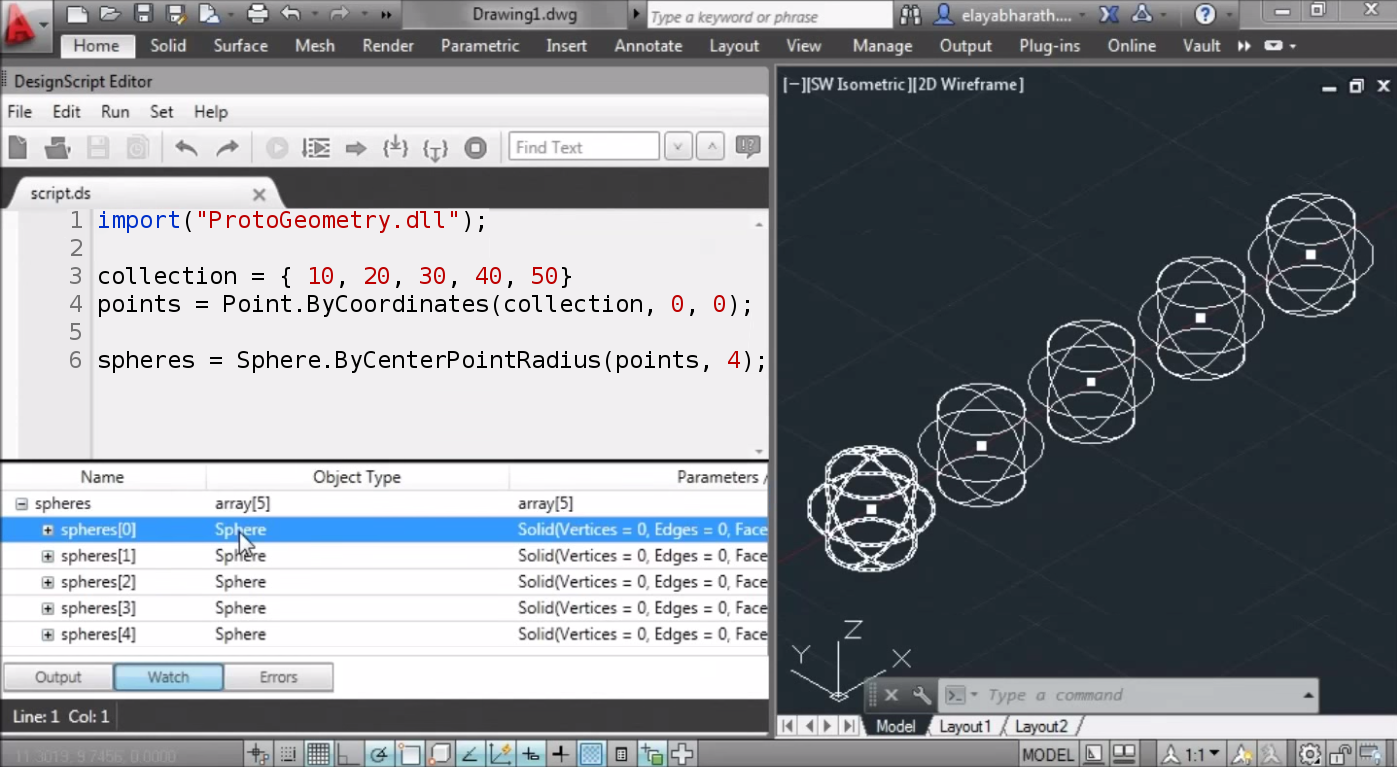
\includegraphics[width=1.0\textwidth]{images/designScriptIDE}
 % \vspace{-15pt}
    \caption{Typical DesignScript programming environment} 
  %  \vspace{-10pt} 
  \label{fig:ds}
\end{figure} 

The programming language is presented as an associative language. The variables are abstract types that can represent numeric values or geometric entities. These variables are maintained in a graph of dependencies. When a change in a variable occurs it forces the re-evaluation of the graph, as shown in Figure~\ref{fig:designscript}, consequently variables has always updated values. This feature is useful, specially in a modeling environment, because it provides continuous feedback to the designer as the model is being modified.

\begin{wrapfigure}{r}{0.45\textwidth}
  %\vspace{-5pt}
  \begin{center}
    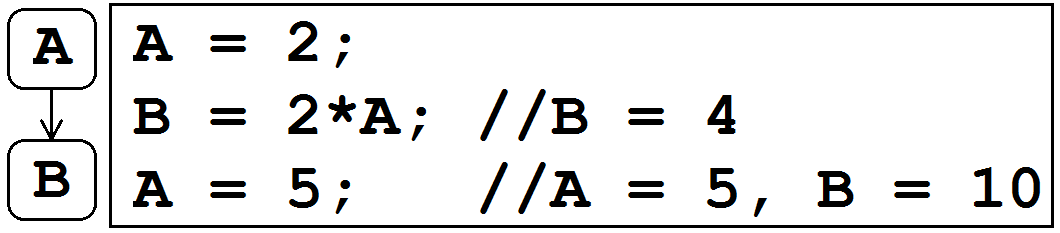
\includegraphics[width=0.45\textwidth]{images/designscript}
  \end{center}
  %\vspace{-20pt}
 \caption{Associative interpretation}  
  %\vspace{-20pt}
    \label{fig:designscript}
\end{wrapfigure}

The DesignScript's programming environment provides a text editor, an interpreter, and a simple debugger. The language interpreter is invoked each time that the designer clicks on the run button. Then all the script is interpreted and its result produces geometric entities rendered in the \gls{cad}. The continuous feedback feature works only in debug mode, because in this mode the script is interpreted line by line. Thus, each update to a variable will change its dependencies and will recompute the model. However, in debug mode the code cannot be edited, so this feature is worthless during code editing.

In the DesignScript's debug mode, users can inspect the variable values by adding \textit{watchers} to them. A watched variable is showed in a special tab, as shown in Figure~\ref{fig:designscript}. In case the variable represents a geometric model, the respective model will be highlighted in the \gls{cad} when the variable is selected. It creates a certain \textit{traceability} between models in the \gls{cad} and code in the editor. In this way the user is able to correlate which model a variable corresponds to. However the inverse, starting form the model and finding the correspondent variable, is unsupported.

DesignScript also supports a typical mechanism of \textit{live} programming environments: the sliders. The sliders are widgets which facilitate giving new values to the program input. This way, designers can create new models reacting to these changes. However, in the DesignScript's sliders the changes are reflected in the models only when the designer leaves the slider. Until then, the designer should imagine how the model would be with the new value, which is completely against the purpose of sliders.

Moreover the DesignScript language, despite of being presented as pedagogic, has some drawbacks. It does not carry any strong metaphor which helps beginners start with the language. Additionally the associative paradigm represents a barrier for sharing code: it discourages the recomposition of modules, because new modules can change the previous one. The environment provides poor mechanisms that help people to find bugs in the code, and finally,  DesignScript is confined to produce geometry in a single \gls{cad} tool.
%%%%%%%%%%%%%%%%%%%%%%%%%%%%%%%%%%%%%%%%%%%%%%%%%%%%%%%%%%%%%%%%%%%%%%%%%%%%%%%%%%%%%%%%%%%%%%%%%%%%%%%%%
\subsection{Monkey} 
\label{subsec:monkey}
Monkey\footnote{\texttt{http://wiki.mcneel.com/developer/monkeyforrhino4}} is a programming environment designed to support \gls{gd}. Like DesignScript, Monkey is used to edit, debug and interpreter scripts. However, Monkey uses RhinoScript as its programming language and Rhinoceros3D\footnote{\label{fnote:rhin}\texttt{https://www.rhino3d.com}} (or Rhino for short), a lighter \gls{cad} than AutoCAD, to generate the geometric models.

Monkey is implemented as a \texttt{.NET} plugin for Rhino4 and provides a programming environment to write and debug scripts. The RhinoScript is based on Microsoft's VBScript language (a descendant of BASIC), and like VBScript it is a weakly typed language. One of the major drawback with this language is the fact that users must beware with the data passed in their functions at all time, because RhinoScript can accidentally casts variables into inappropriate types. Therefore, it creates errors difficult to find, specially for people which are learning to program.

Monkey is based on general-purpose programming environments. It provides typical features of those environments, namely syntax highlighting, auto-completion, and error highlighting. The organization of code into trees is also similar. However, the programming environment and language, does not provide any well designed feature which helps beginners to start with programming. The provided features are based on general-purpose systems, instead of being tailored for \gls{gd}.
%%%%%%%%%%%%%%%%%%%%%%%%%%%%%%%%%%%%%%%%%%%%%%%%%%%%%%%%%%%%%%%%%%%%%%%%%%%%%%%%%%%%%%%%%%%%%%%%%%%%%%%%%
\subsection{Rosetta}
\label{subsec:rosetta}
Rosetta~\citep{lopes2011portable} is a programming environment designed to support \gls{gd} that is based on DrRacket~\citep{findler2002drscheme}. Like Monkey, Rosetta provides its own environment detached from the \gls{cad}. Rosetta is a step forward from the previous systems, because it solves the portability problem among \gls{cad} tools. In Rosetta a \gls{gd} program can be written in various programming languages (frontends) and the geometric models can be rendered by various \glspl{cad} (backends). As a result, designers are free to write their programs in their preferred frontend which, upon execution, will generate the same geometry for the various backends. In Figure~\ref{fig:rosetta}, a program is written in Racket and its execution produces geometry for AutoCAD.

\begin{figure}[!htbp]
%\vspace{-5pt}
  \centering
  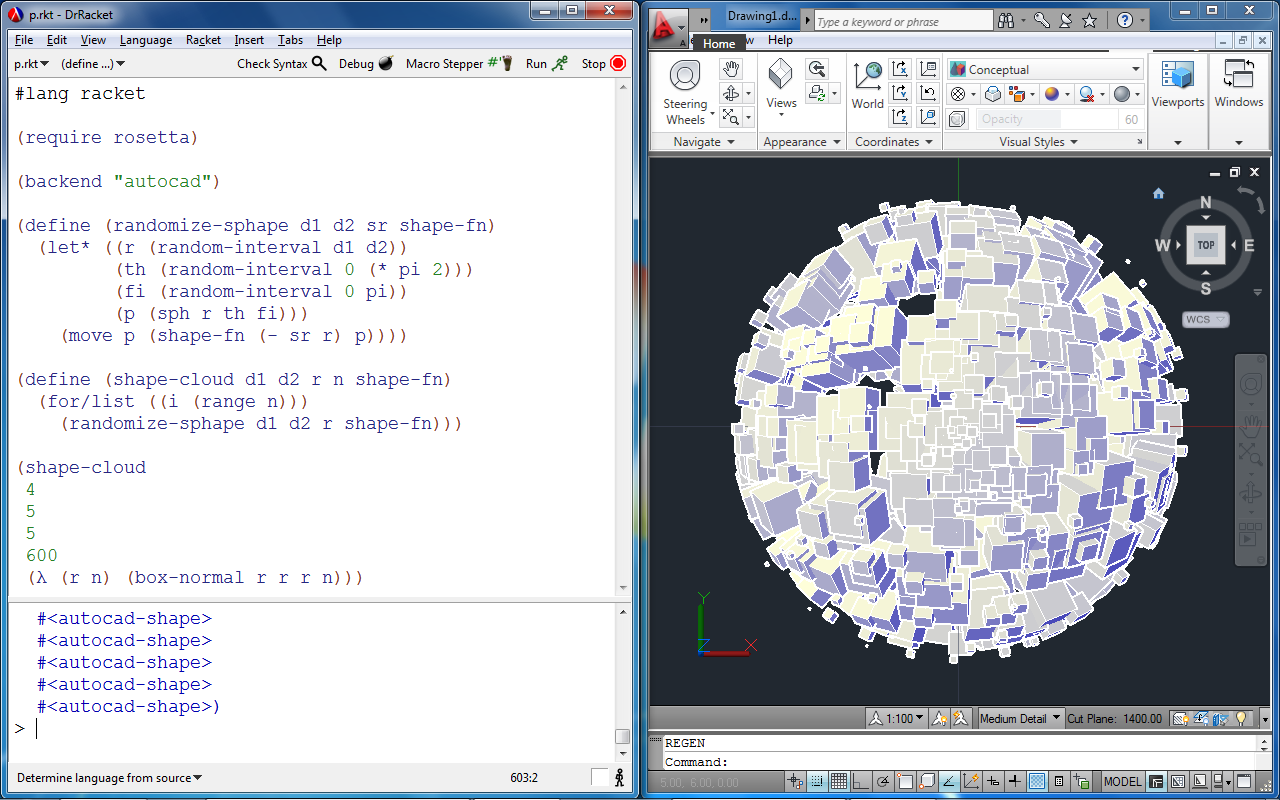
\includegraphics[width=1.0\textwidth]{images/rosetta1}
  %\vspace{-20pt}
    \caption{Rosetta programming environment.}  
  \label{fig:rosetta}
  %\vspace{-10pt}
\end{figure} 

Rosetta has been used to teach programming in architecture courses. Tailored to this end, Rosetta uses DrRacketas its own programming environment. The DrRacket environment serves a number of functions, but the most important is that the student can start immediately to learn programming. For instance, the environment is set up with just three lines of code. As shown in Figure~\ref{fig:rosetta}, the \texttt{\#lang} specifies the frontend language, the \texttt{require} imports Rosetta's primitives and finally the \texttt{backend} names a possible backend.

The Racket language is also an advantage of Rosetta's environment, because it encourages the use of the mathematical paradigm for writing algorithms. In this way, students that learn simple programming techniques, such as recursion, are able to create robust models. Additionally, as the students progress, new programming languages are also available to learn, such as JavaScript, Python, Processing, and so on.

The Rosetta's environment provides some interesting tools for \gls{gd}, such as a programming flow tracer, similar to the DesignScript's watcher. It highlights models in the \gls{cad} upon selection of expressions, it also supports the inverse, selecting the model in the \gls{cad} and shows the expression in the code editor. Another interactive tool is the slider, an attempt to provide immediate feedback to the designers. It uses the DrRacket slider, associating the slider callback to the function that generates the entire model, so each time the slider change a new model will be generated. However, this process must be performed manually.

Undoubtedly Rosetta's environment goes further than the textual environments for \gls{gd} presented in this report. However it presents some drawbacks which may discourage the learning in general. Beginning with the usual programming language: Racket. The syntax of a Racket program represents a significant barrier for reading. For instance the function which draws a circle in Rosetta is written as \texttt{(circle (xy 0 0) 1)}. The reader must lookup or memorize every argument. Using the Rosetta's documentation the reader will spend even more time, because it is in a book mixed with architecture topics.
%%%%%%%%%%%%%%%%%%%%%%%%%%%%%%%%%%%%%%%%%%%%%%%%%%%%%%%%%%%%%%%%%%%%%%%%%%%%%%%%%%%%%%%%%%%%%%%%%%%%%%%%%
\subsection{Grasshopper}
\label{subsec:grasshopper}
Grasshopper\footnote{\texttt{http://www.grasshopper3d.com/}} is a programming language and environment designed to support \gls{gd} using a visual language. Grasshopper provides an alternative way to programming. By definition, it is a bi-dimensional representation consisting of iconic components that can be interactively manipulated by the user according to some spatial grammar~\citep{myers1990taxonomies}. For example, the boxes in Figure~\ref{fig:grass} are components which receive the input (left ports) perform some operations and return the output (right port). The components are linked to other components establishing a \textit{dataflow} paradigm where the input of a component is the output of another.

\begin{figure}[!htbp]
%\vspace{-5pt}
  \centering
  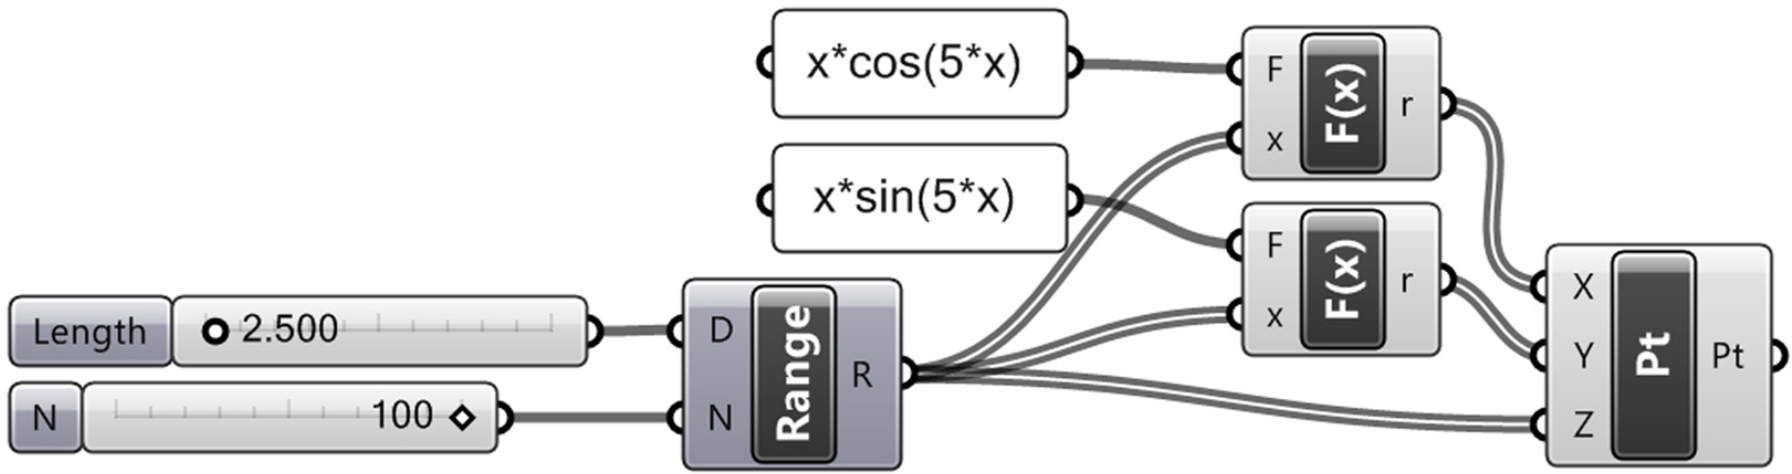
\includegraphics[width=0.8\textwidth]{images/grasshopper}
  %\vspace{-5pt}
    \caption{A program in Grasshopper that computes the 3D coordinates of a conical spiral. Each time the left sliders are dragged a new coordinate is calculated.}
  \label{fig:grass}
  %\vspace{-10pt}
\end{figure}

Like Monkey, Grasshopper is implemented as a \textit{plugin} for Rhino$^{\ref{fnote:rhin}}$. However Grasshopper tailors the Rhino's environment with specific \gls{gd} tools. These tools are state of the art, because they implement important principles for design models, such as the following:

\begin{itemize}
 \item \textit{Get immediate feedback}. As the user interacts with the components, by adding and connecting them, the result reflects immediately in the \gls{cad} model. It facilitates the design conception, because the user's intentions are immediately visible. 
 \item \textit{Facilitate program input}. To facilitate the process of design exploration, Grasshopper provides sliders which are connected at the component input. Dragging the slider causes a change propagation through components. The components are re-executed with the new slider value. Combined with the above feature new models are generated immediately.
 \item \textit{Correlate the program with the generated elements}. Like DesignScript's watcher, by selecting a component its geometry is highlighted in the \gls{cad}. It allows designers to better understand a program by figuring out the roles of each component.
 \item \textit{Show comparisons between models}. Grasshopper provides a special component that, when connected at the output of another component, replicates the geometry. This mechanism is useful for design exploration, because it maintains in the \gls{cad}'s background an old replica of the changed geometry. It adds a context at each change, so the designer can compare the result of his change in the new geometry based on the old one.
\end{itemize}

Mainly, the Grasshopper interactivity depends on the immediate feedback tool. However, this tool will never scale for arbitrarily complex programs, because the \gls{cad}'s render is not designed to process the huge amount of information generated by \gls{gd} methods. Other systems, such as DesignScript and Rosetta, improve this problem by sidestepping most of the functionality of traditional \gls{cad} tools and focusing only on the generation and visualization of geometric models. These systems provide a backend based on OpenGL that is independent of a full-fledged \gls{cad} application, but, in Grasshopper, there is no such backend.

Moreover, the traceability among components is just in one direction. From the designer perspective, it would be more useful start form the geometry and find which component implements it, but it is unsupported. However, despite the usefulness of model comparison in design exploration, this feature is also unsupported.
%%%%%%%%%%%%%%%%%%%%%%%%%%%%%%%%%%%%%%%%%%%%%%%%%%%%%%%%%%%%%%%%%%%%%%%%%%%%%%%%%%%%%%%%%%%%%%%%%%%%%%%%%
\subsection{Dynamo}
\label{subsed:dynamo}
Dynamo\footnote{\texttt{http://dynamobim.com/}} is a programming language and environment designed to support \gls{gd}. Like Grasshopper, Dynamo provides an alternative way to programming. However Dynamo, like DesignScript, is implemented on top of Revit, an Autodesk product for \gls{bim}.

\begin{wrapfigure}{r}{0.5\textwidth}
  %\vspace{-30pt}
  \begin{center}
    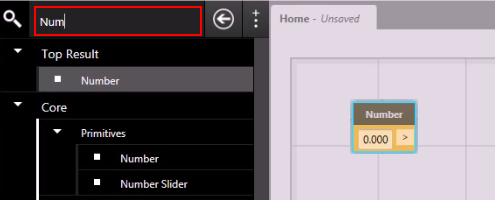
\includegraphics[width=0.5\textwidth]{images/dynam-tab}
  \end{center}
  %\vspace{-18pt}
 \caption{Dynamo search tab. Searching for a component, highlighted in red.}  
  %\vspace{-20pt}
    \label{fig:dynam}
\end{wrapfigure}

Dynamo provides a set of tools similar to Grasshopper, particularly a searching table, as shown in Figure~\ref{fig:dynam}, which provides quick access to the primitives of the language, such as the components and widgets. This feature encourages designers to explore the available components and try new components.

In general, Dynamo and Grasshopper are programming environments and visual languages popular among novices in programming. The smooth learning curve and perhaps the style of the \gls{ui} elements are attractive for beginners. However as the visual programs become large and complex it requires more time to understand, maintain, and adapt to new requirements, than the textual programs as showed in~\citep{leitao2011programming}. Despite spending more time and effort to learn a textual programming language, the learners have their time quickly recovered once the complexity of the design task becomes sufficiently large.
%%%%%%%%%%%%%%%%%%%%%%%%%%%%%%%%%%%%%%%%%%%%%%%%%%%%%%%%%%%%%%%%%%%%%%%%%%%%%%%%%%%%%%%%%%%%%%%%%%%%%%%%%
\subsection{Mathematica}
\label{subsec:mathematica}
Mathematica~\citep{wolfram1991mathematica} is a language and environment built to support scientific calculation. It is widely used in the scientific community, specially by students, because it represents programs using a short and clear artificial language. This language supports not just linear textual input, but also two-dimensional input, like traditional mathematical notation.

\begin{figure}[!htbp]
%\vspace{-5pt}
  \centering
  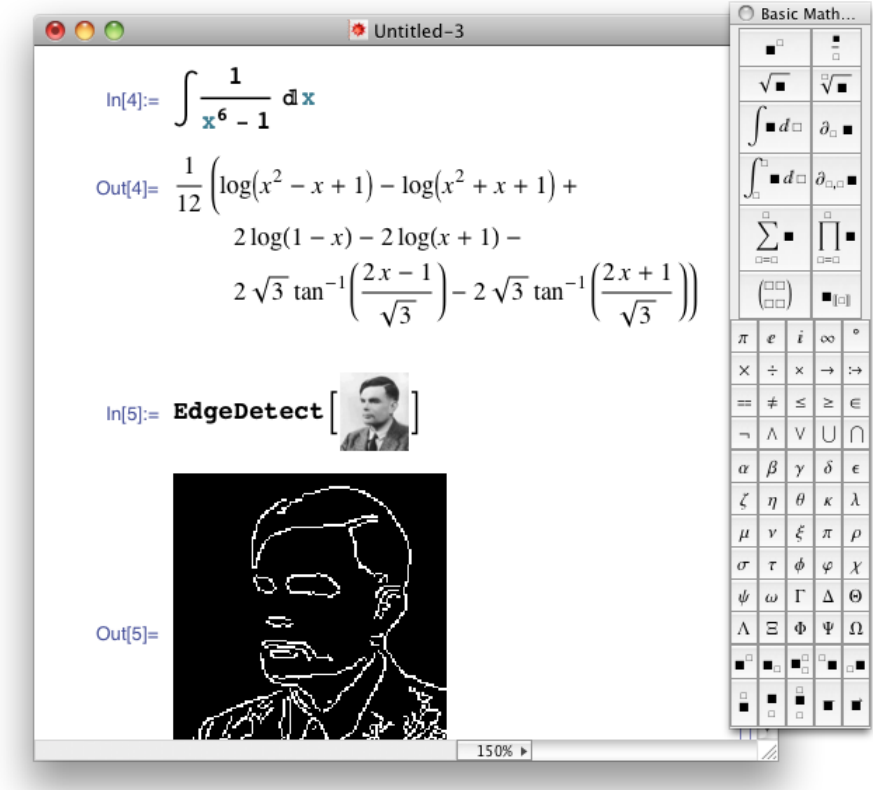
\includegraphics[width=.7\textwidth]{images/mathematica}
  %\vspace{-20pt}
    \caption{Mathematica notebook}  
  \label{fig:math}
  %\vspace{-10pt}
\end{figure} 

The core concepts of Mathematica are based in the paradigm initiated by Turing's work~\citep{wolfram2003wolfram}. In this paradigm mathematical processes are systematized as computations. For example, in a typical interaction, the user types a mathematical expression in the Mathematica environment (i.e. notebook), then this expression is evaluated, as shown in Figure~\ref{fig:math}.  

A relevant aspect of Mathematica's notebook is the immediacy that users get a response. Unlike a typical program that must be executed explicitly to get a feedback of an action, in this notebook expressions are evaluated as soon as they are typed. It works like a read-eval-print loop, however it has enhanced mechanisms to present data meaningfully.

The Mathematica features are well designed to present data in a human readable form. It would be useful for an external programming languages, if it could take advantage of these features. Unfortunately, Mathematica is closed for this end.
%%%%%%%%%%%%%%%%%%%%%%%%%%%%%%%%%%%%%%%%%%%%%%%%%%%%%%%%%%%%%%%%%%%%%%%%%%%%%%%%%%%%%%%%%%%%%%%%%%%%%%%%%
\subsection{IPython}
\label{subsec:ipython}

IPython~\citep{PER-GRA:2007} is a programming environment built to support scientific calculation. Unlike Mathematica~\citep{wolfram1991mathematica},  IPython is an open platform for extensions, it allows external programming languages (frontends) to use its features which includes an interactive shell, and a browser-based notebook with support for code, text, mathematical expressions, plots, and other rich media. 

Like Mathematica, IPython has a notebook where users can try out expressions and immediately see its result, as shown in Figure~\ref{fig:ipython}, however this notebook is in a web format. IPython's architecture is a typical client-server, where the frontend is the client (i.e. the notebook), and the server is a language kernel (i.e. the programming language which users interact with). The communication between client and server, is through a strict protocol that the language kernel must implement. 

\begin{figure}[!htbp]
  \centering
    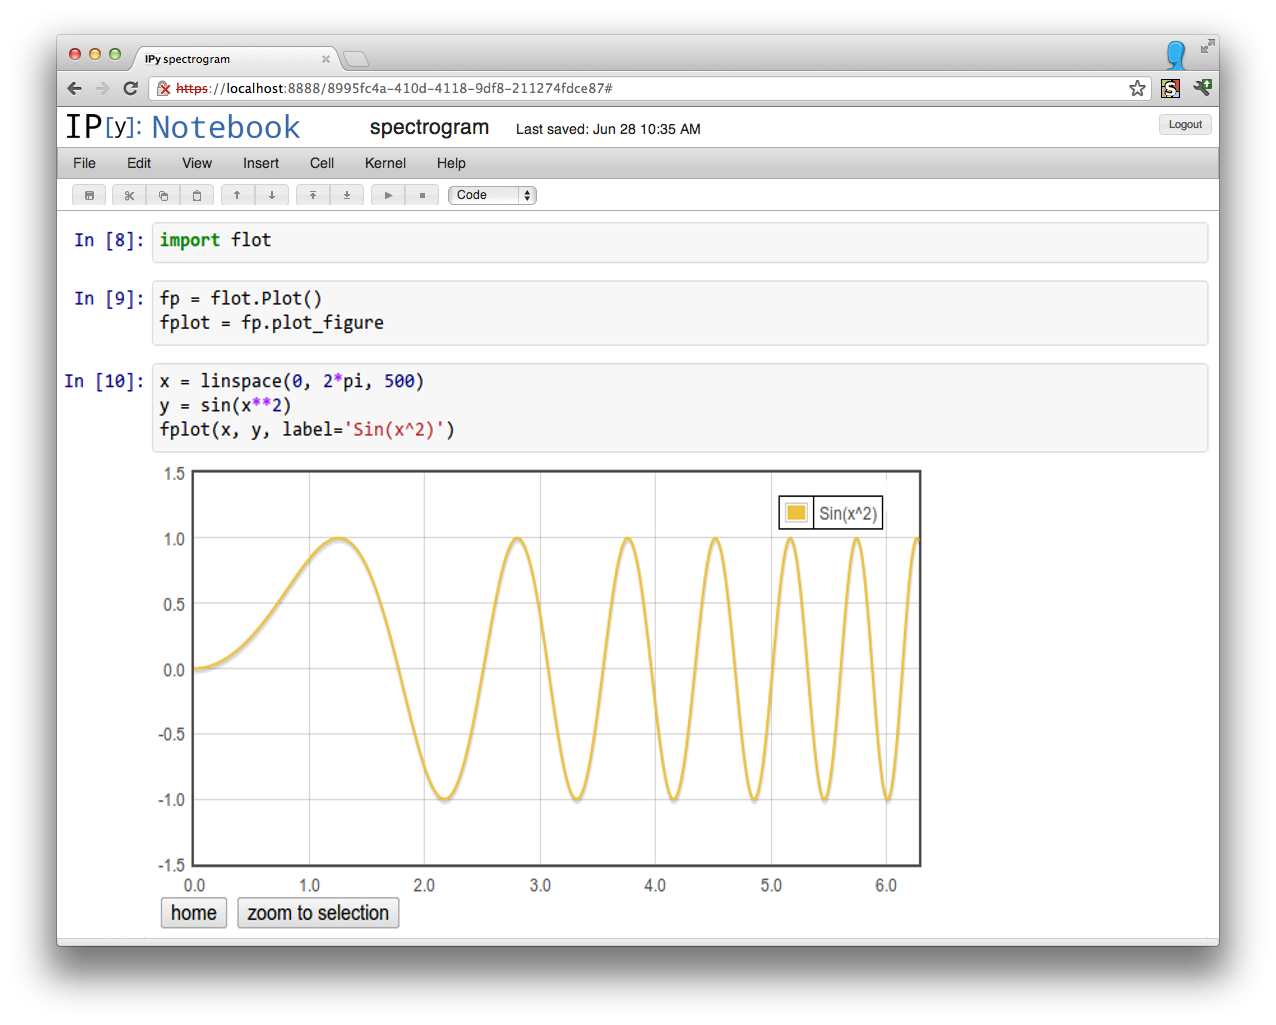
\includegraphics[width=0.7\textwidth]{images/ipython}
 \caption{IPython browser-based notebook}
    \label{fig:ipython}
\end{figure}

IPython provides a base layer for new programming environments, by exposing the major components of its architecture, consequently its features are available from other systems. For example, IJulia uses IPython interface with Julia language. 
%%%%%%%%%%%%%%%%%%%%%%%%%%%%%%%%%%%%%%%%%%%%%%%%%%%%%%%%%%%%%%%%%%%%%%%%%%%%%%%%%%%%%%%%%%%%%%%%%%%%%%%%%
\subsection{MathCAD}
\label{subsec:mathcad}
MathCAD\footnote{\texttt{http://www.ptc.com/product/mathcad}} is a programming environment and language built to support scientific calculation. Like Mathematica, MathCAD aims to present information into a human readable form. However, it generates live calculations with graphical plots, text and images into a single document. This document is the program environment as well as the final product.

The mathematical expressions defined in the MathCAD document act as an associative language. So, when an expression is changed its value is propagated through the document. This mechanism is the base of the interactiveness. However, it represents a barrier for program recomposition, because new expressions can change the previous ones. That means that variables has a global scope, the MathCAD document, if in somewhere a variable is changed it will be changed in every occurrence in the document.   
%%%%%%%%%%%%%%%%%%%%%%%%%%%%%%%%%%%%%%%%%%%%%%%%%%%%%%%%%%%%%%%%%%%%%%%%%%%%%%%%%%%%%%%%%%%%%%%%%%%%%%%%%		     
\section{Summary}

Table~\ref{tab:sum} shows the presented systems based on their major design influences. The table is also intended to address the following questions:

\begin{table}[h]
%\vspace{0pt}
\centering
%\ra{1.0}
\resizebox{\textwidth}{!}{%
\begin{tabular}{@{}clllc@{}}
\toprule
\multicolumn{1}{l}{{\bf Type$^{(1)}$}} & {\bf System} & {\bf Main feature$^{(2)}$} & {\bf \begin{tabular}[c]{@{}l@{}}Support to understand \\ programs$^{(3)}$\end{tabular}} & {\bf Representation of code$^{(4)}$} \\ \midrule
\multirow{6}{*}{GS} & Eclipse & \multirow{4}{*}{\begin{tabular}[c]{@{}l@{}}support software \\ development life cycle\end{tabular}} & \multirow{4}{*}{debugger} & \multirow{16}{*}{text} \\
 & NetBeans &  &  &  \\
 & IntelliJ &  &  &  \\
 & MVS &  &  &  \\ \cmidrule(lr){2-4}
 & Xcode & \multirow{2}{*}{observable programming} & \multirow{2}{*}{live execution feedback} &  \\
 & LightTable &  &  &  \\ \cmidrule(r){1-4}
\multirow{7}{*}{TS} & LOGO & \multirow{2}{*}{understandable language} & \multirow{2}{*}{physical interpretation} &  \\
 & SmallTalk &  &  &  \\ \cmidrule(lr){2-4}
 & Processing & \multirow{2}{*}{visual context} & \multirow{2}{*}{instant visualization} &  \\
 & Fluxus &  &  &  \\ \cmidrule(lr){2-4}
 & DrRacket & gradual learning & debugger; stepper &  \\ \cmidrule(lr){2-4}
 & PythonTutor & \multirow{2}{*}{show program flow} & \multirow{2}{*}{\begin{tabular}[c]{@{}l@{}}navigate through the \\ program execution\end{tabular}} &  \\
 & YinYang &  &  &  \\ \cmidrule(r){1-4}
\multirow{8}{*}{ES} & DesignScript & \multirow{3}{*}{\begin{tabular}[c]{@{}l@{}}support generative design \\ methods\end{tabular}} & \multirow{3}{*}{debugger} &  \\
 & Monkey &  &  &  \\
 & Rosetta &  &  &  \\ \cmidrule(l){2-5} 
 & Grasshopper & \multirow{2}{*}{\begin{tabular}[c]{@{}l@{}}alternative way to \\ expressing programs\end{tabular}} & \multirow{2}{*}{dataflow paradigm} & \multicolumn{1}{l}{\multirow{2}{*}{graphical components}} \\
 & Dynamo &  &  & \multicolumn{1}{l}{} \\ \cmidrule(l){2-5} 
 & Mathematica & \multirow{3}{*}{\begin{tabular}[c]{@{}l@{}}support scientific \\ calculation\end{tabular}} & \multirow{3}{*}{present data meaningfully} & \multicolumn{1}{l}{\multirow{3}{*}{mathematical forms}} \\
 & IPython &  &  & \multicolumn{1}{l}{} \\
 & MathCAD &  &  & \multicolumn{1}{l}{} \\ \bottomrule
\end{tabular}
}
%\vspace{1pt}
\caption{System attributes}
%\vspace{-20pt}
\label{tab:sum}
\end{table}

(1) \textit{What is the purpose of the system?} We categorized three main purposes for a system. \gls{gs} designed for building complex software for the industry; \gls{ts} designed to help people learn how to program; \gls{es} designed to help people build things that are tailored to their own needs.

(2) \textit{How does the system support its purpose?} We identified the following strategies: (i) support software development life cycle, (ii) turn programming in something more observable, (iii) create an understandable language, (iv) combine textual programming with a visual context, (v) support gradual learning in a single environment, (vi) show the program flow, (vii) support generative design methods, (viii) find alternative ways for to express programs, and (ix) support scientific calculation.

(3) \textit{Does the programming environment provide additional support to enable users to better understand the behavior of their programs?} Environments in our study used several techniques to help users understand the behavior of their programs. These included (i) a debugger which helps to find bugs in the program, (ii) an enhanced debugger which provides live execution feedback, (iii) languages with strong metaphor allowing physical interpretation, (iv) instant visualization of models, (v) navigation through the program's execution (vi) assembling components in a dataflow paradigm and (vii) present data adequately.

(4) \textit{How does code look in the programming environment or language?} The systems in our study represent programs using text, users can type, graphical components, users can manipulate, and mathematical forms users can fill in.

\section{Conclusion}

In the surveyed systems, the common representation of code is textual. This representation is typically static and, to be understood, requires the reader to know the vocabulary of the programming language. For a novice it is simply a barrier to learning. On the other hand, the representation of programs as graphical components or mathematical forms lowers this barrier, because for simple programs it is easier to read, but it becomes incomprehensible as the program grows.
%TEX root = ../dissertation.tex

\iffalse \bibliography{bibliography/dissertation} \fi

\chapter{Designing a Programming Environment for Generative Design}
\label{chapter:pegd}

\section{Design Principles} 

Programming is hard to learn. Unfortunately, as shown in the previous section, few programming languages or environments are designed to introduce the basics of good software engineering practice. Specially in Architecture, the environments used to support \gls{gd} either they are old or obsolete, or they enforce particular programming methods that are inadequate, or they are not pedagogic, meaning that they are not designed for the particular programming skills of the \gls{gd} community.

The literature is vast, but it is clearly divided in two perspectives: software engineering perspective, or psychological/educational perspective. That means either systems designed for expert programmers~\citep{carlson2005eclipse,intellij2001intellij,lighttable,boudreau2002netbeans,guckenheimer2006software}, or systems designed for novices~\citep{papert1980mindstorms,goldberg1983smalltalk,GuoSIGCSE2013,Reas2006}. The problem is that while programming systems designed for expert programmers are constantly updated, systems designed for novices are usually obsolete or in disuse. It negatively affects other communities that are not focused on develop software for industry, but for their own purpose which includes mainly novice users.

For example the \gls{gd} community is focused on build software to support Architecture methods, however designers are in desperate need of a programming system that correspond their needs. These needs are from different natures for instance: give support to the increasing adoption of \gls{gd} methods, deal with the increasingly complexity of current \gls{gd} programs, support tools that allows programs to be tested quicker, among others.

In the next section I propose...

\section{Program Documentation}

Program documentation is a software requirement of the utmost importance because it is a key factor for understanding programs. Even the best program, the most perfectly suitable for the job, will be essentially useless if the people who need to use it do not know what it is; cannot understand it well enough to use, build, or modify it; or (worst of all) misunderstand it and apply it incorrectly. And all of the effort, analysis, hard work, and insightful design spend to construct it will have been wasted.

Software exists for a specific reason and documentation exists to explain this reason. Every piece of code has its rational and a reason to be written in that way. Then the documentation recollects all these rationales organizing them in a form of different artifacts such as, requirements description, architectural models, data models, \gls{api} documentation, flow diagrams, use case diagrams, etc. So it is undoubtedly a rich source of information not only for the developer who did the software but also for the developer who will test the application, for the stakeholder who will use the application, and eventually for the developer who will maintain that code.

In fact software maintenance, traditionally defined as any modification made on a system after its delivery, is a dominant activity in software engineering. Some reports place maintenance at 90\% of the total cost of a typical software project~\citep{seacord2003modernizing,pigoski1996practical}. One of the main difficulties in software maintenance is a lack of up-to-date documentation~\citep{de2005study}. As a result, some studies indicate that 40\% to 60\% of maintenance activity is spent simply studying existing software~\citep[p. 475 and p. 35 respectively]{pigoski1996practical,pfleeger1998software}. Having an updated documentation would dramatically reduce the effort spent in this study, helping the developer to comprehend the code and maintain it.

The sad truth is that writing program documentation today is perceived as a tiresome task, if it is done at all, is often treated as an afterthought, something people do because they have to~\citep{sousa1998survey}. Bass et al. summarizes many possible reasons that lead programmers to write the documentation, and then concluded as follows:

\blockquote{Maybe a contract requires it. Maybe a customer demands it. Maybe a company's standard process calls for it. In fact, these may all be legitimate reasons. But none of them are compelling enough to produce high-quality documentation.~\citep[p. 327]{BassClementsKazman201210}}

Producing a high-quality documentation should be a natural developer's attitude not because it's ``required" but because they see that it is essential to the matter at hand. The documentation defends the developer's job because it speaks for him, for example in agile methods it can be used as contract~\citep{ambler2007agile}. It also helps developers reason about the architecture design of their programs, and communicate these ideas while the development is in progress. However produce useful documentation is a hard task and developers have to consider that some documentation artifacts are more important than others.

As described earlier, documentation is composed by several artifacts, formally defined as any artifact intended to communicate information on the software system~\citep{forward2002relevance}. This communication is aimed at human readers, from the technical document delivered to the developer team, until the user manual delivered to the users. But the central point from where the documentation comes from is the source code, as a result it is the most important artifact as confirmed in the following study:

\blockquote{Source code and comments are the most important artifact to understand a system to be maintained. Data model and requirement description were other important artifacts. Surprisingly, and contrary to what we found in the literature, architectural models and
other general view of the system are not very important. This could simply indicate that such documentation artifacts are used once to have a global understanding of the system and never consulted again after.~\citep[p. 74]{de2005study}}

The importance of source code and comments is a reality already noted in the software industry, so the use of automation tools to generate, verify, and maintain the source code documentation, is a common practice. The most frequently cited technologies, as concluded in~\citep{forward2002relevance}, are Javadoc\footnote{\texttt{http://docs.oracle.com/javase/7/docs/technotes/guides/javadoc/}} and DocWiz\footnote{\texttt{http://docwiz.sourceforge.net/}} to comment Java source code, Doc++\footnote{\texttt{http://docpp.sourceforge.net/}} and Doxygen\footnote{\texttt{http://www.stack.nl/dimitri/doxygen/index.html}} to comment source code in languages such as C, C++, and also Java. These tools generate an on-line documentation browser (in HTML) and/or an off-line reference manual (in $\mbox{\LaTeX}$) from a set of documented source files. The comments are inserted directly in the source code between a start tag and a end tag. These tags typically use the language's comment delimiter to prevent any compilation error, once the compiler will ignore any word between comments. In case of Javadoc an extra asterisk is needed to generate the documentation, so the comments are embed inside \texttt{/** ... */} (as shown in Figure~\ref{fig:javadoc-code}). Additionally, other tags are provided to document for example the function parameters (\texttt{@param}), the function return (\texttt{@return}), an exception that may be thrown from the method (\texttt{@exception}, \texttt{@throws}), and so on. As a result, these tags add proper information into the HTML page (e.g. as shown in Figure~\ref{fig:javadocgen}).

\begin{figure}
\centering
\begin{subfigure}{.5\textwidth}
  \centering
  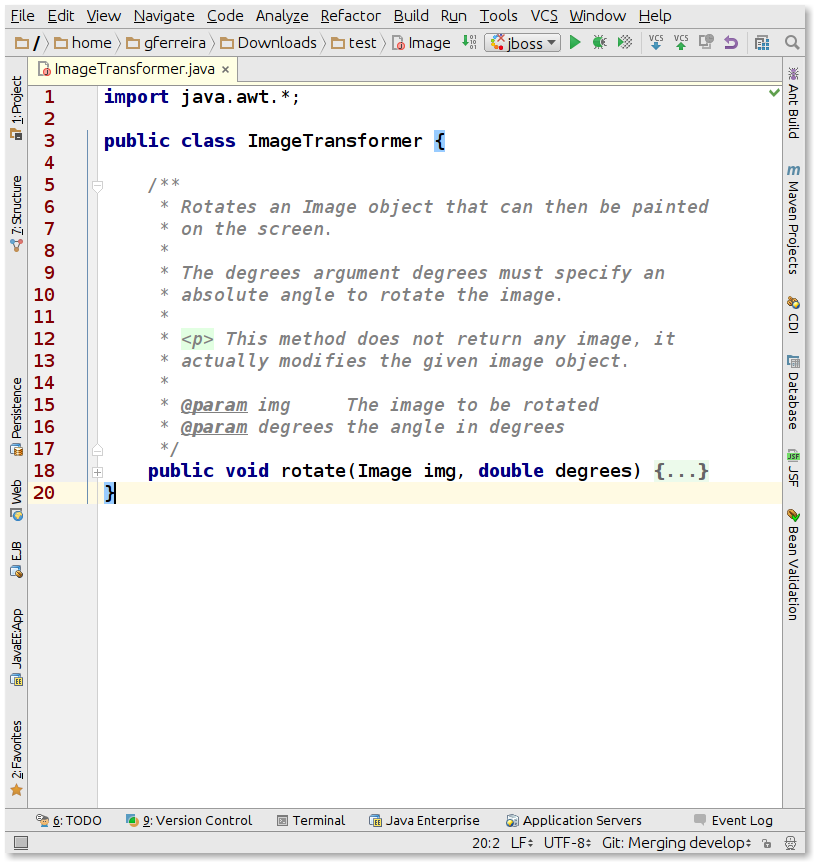
\includegraphics[width=.9\linewidth]{images/javadoc-code}
  \caption{A Javadoc annotation of a Java method}
  \label{fig:javadoc-code}
\end{subfigure}%
\begin{subfigure}{.5\textwidth}
  \centering
  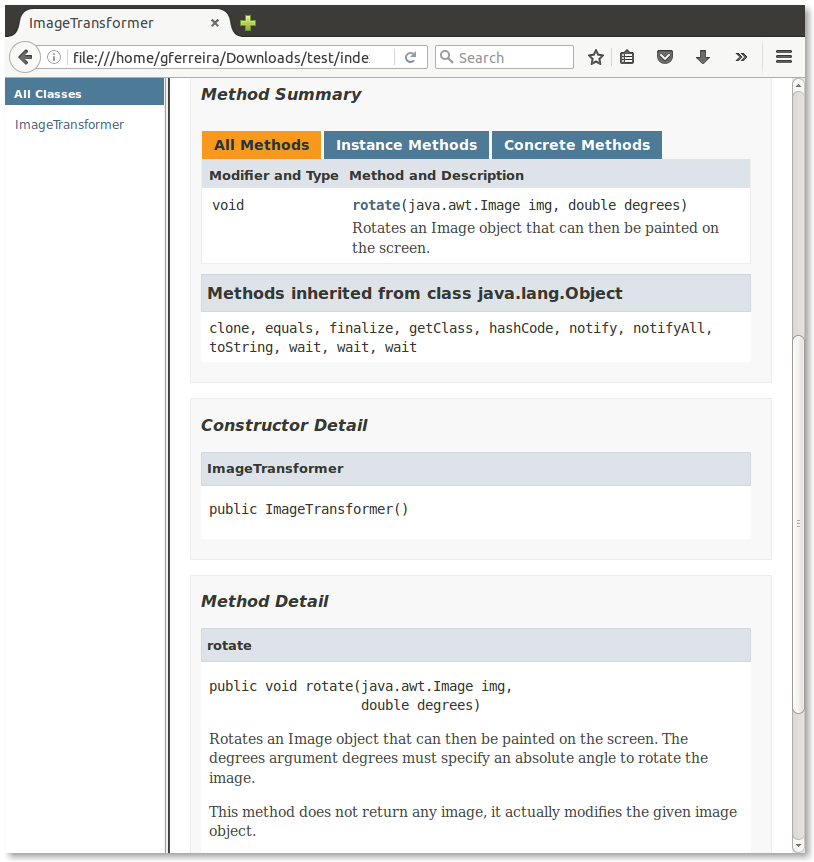
\includegraphics[width=.9\linewidth]{images/javadoc}
  \caption{Javadoc HTML auto-generated}
  \label{fig:javadocgen}
\end{subfigure}
\caption{Javadoc generation of a HTML page from a documented Java method. In the left is the source code commented with the opening tag \texttt{/**}, in the right is the generated documentation page.}
\label{fig:javadoc}
\end{figure}

Figure~\ref{fig:javadoc} shows an example of Javadoc an industry standard tool which provides interesting functionalities for documenting Java classes. The HTML format keeps information together giving the convenience of being able to hyperlink related documentation. As a result, programmers can easily navigate through classes and their respective methods. Moreover, Javadoc provides a widely integration trough \glspl{ide} (e.g. Eclipse, IntelliJ, NetBeans, etc), being able to generate automatic comments and the proper documentation using these \glspl{ide}. This tool indeed helps to produce a presentable documentation without much effort, however there are clearly important points to improve.

In these tools, the documentation are essentially represented as rows of plain text. Despite of supporting HTML format for generating the final documentation, there is no rich media resource in the generated pages only text and hyperlinks to other pages. Moreover, the developer's attention is taken from code into a series of static pages that do not add more information, actually they show less than the source code. And the automatic comments generated by \glspl{ide} are useless comments that do not add any rigorous information for the developer (e.g. a method called \texttt{getFoo()} would be commented as ``This method gets a foo"). Finally, these tools are more focused on creating an industry standard documentation mainly devoted to the client, than focused on creating a useful documentation that effectively helps developers to comprehend the code and its architecture.

The representation of source code dramatically affects its comprehensibility and usability~\citep{baecker1986design}. The idea of enhancing program comprehension and usability by improving its representation using richer media resources is not new in the literature~\citep{marcus1982graphic,baecker1986design,baecker1983enhancing}. These researches define design principles for enhancing program visualization, showing the impact of those principles in the readability of the code. Based on these works, subsequently researches and implementations have been tried to keep those principles alive inside the academic context. For example Barista~\citep{ko2006barista} implements some of these principles  allowing media-rich annotation in the code editor (see Figure~\ref{fig:barista}), while Codelets~\citep{oney2012codelets} focus on supporting media-rich resources in code completion by enabling HTML icons visualization (see Figure~\ref{fig:codelet}) helping developer to write HTML pages 43\% faster than when using a standard Web browser\citep{oney2012codelets}.

\begin{figure}
\centering
\begin{subfigure}{.5\textwidth}
  \centering
  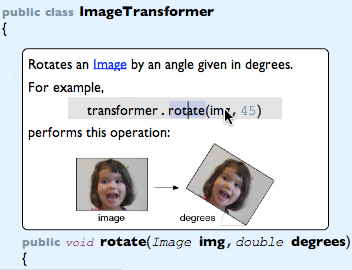
\includegraphics[width=.7\linewidth]{images/barista}
  \caption{A media-rich annotation in the Barista editor}
  \label{fig:barista}
\end{subfigure}%
\begin{subfigure}{.5\textwidth}
  \centering
  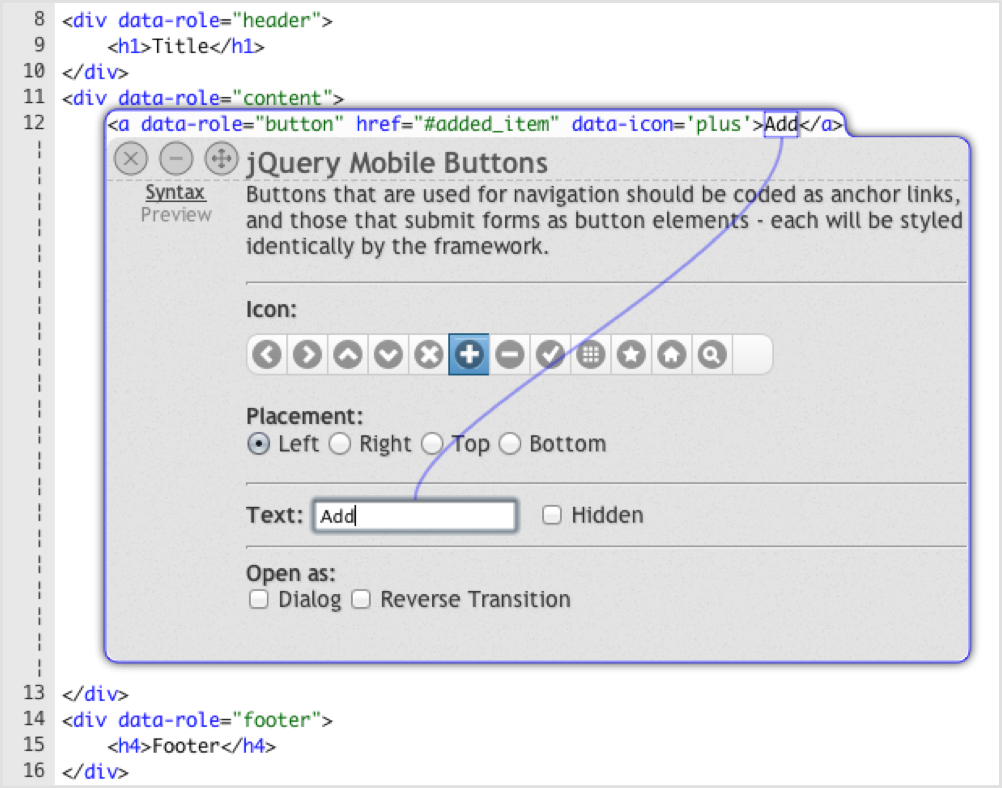
\includegraphics[width=.7\linewidth]{images/codelet}
  \caption{A Codelet inline helper}
  \label{fig:codelet}
\end{subfigure}
\caption{Example of media-rich annotations supported by code editors. On the left is Barista editor showing a Java method with richer annotations including images. On the right is the Codelets implementation showing the inline helper with icons defined for mobile buttons.}
\label{fig:richmedia}
\end{figure}

Barista~(Figure~\ref{fig:barista}) proposes a framework for creating interactive tools. It is build on top of Citrus~\citep{ko2005citrus}, a programming language intentionally created for supporting the creation of structured editors, consequently it is a positive factor that facilitates the implementation of the proposed tools. These tools implement several principles of usability and readability, for example media-rich annotation of methods (including hyperlink and diagrams inside the comments; allowing show/dismiss the comments by double clicking), readable pretty-printed view of formulas (enabling edit of these expressions by double clicking), and so on. However Barista seams to be more a prove of concept, than actually a system used nowadays, besides the programming language used in this implementation be probably obsolete. On the other hand, Codelets~(Figure~\ref{fig:codelet}) uses media-rich resources to present in a pop-up a variety of icons that develops can choose to create their web pages. However it is more related with code completion technologies than properly support program documentation.

The lack of tools that properly document a program is still a problem that negatively affects the \gls{gd} area. There is no such a tool which properly documents a program or automates the process of documentation. However the implementation of this tool and many other potentially useful tools are difficult or impossible in programming environments like DesignScript~\citep{aish2012designscript}, Monkey (and other textual environments used in \gls{gd}) that visually represent source code as rows of plain text. In the other hand, the visual programming languages, supported by environments such as Grasshopper and Dynamo, represent the source code visually with boxes and lines. However, to document these visual programming languages usually a box of plain text are provided, so that users can place it any where at program. As a result, the program documentation becomes spread in a bunch of boxes randomly placed around the program components, clearly an avoidable way to document a program.

This problem is aggravated by the increasing use of \gls{gd} methods to support the design and conception of real architectural projects. The architectural projects, in the likeness of software projects, has a design phase where architects study the problem which they want to solve, analyze eventual constraints imposed by the client or even by external factors, and then define a draft of the solution. At the end of this process several artifacts are produced, is commonly expected diagrams and handmade sketches (as those portrayed in Figure~\ref{fig:sketch-fig}). These sketches are commonly used among architects since early days of architecture~\citep{do2001thinking}, because they represent a compact medium to convey complex ideas. The information generated in the design phase can be sufficient enough to model and construct the entire project serving as a start point, and a basis, to develop the project. 

For example, the Figure~\ref{fig:sketch-using} (reference here) shows the importance of this phase in the architectural conception. In this example the architect started by drawing a series of  sketches annotating them with dimensional and spacial parameters such as height ($h$), diameter ($d$), the normal vector ($\vec{N}$), and vertex points (e.g. $P_0, P_1, P_2, ...$) of each shape (see Figure~\ref{fig:sketch-fig}). Then he used those shapes, as a small piece of design, by combining them to create a distinct pattern. After, he used this pattern by applying it into a 2D sinusoidal surface which represents the ceiling of a geometric structure, as shown in Figure~\ref{fig:sketch-fig-result}. In this example is also clear the known approach in software engineering: dive to conquer, because the architect started by designing the small pieces of the model and then he combined those unities of design to project the final structure. Each piece was carefully designed to join with the whole model, it is important to understand what is the meaning of those annotations to realize how can I propose a useful tool that effectively helps in the program documentation.

\begin{figure}
\centering
\begin{subfigure}{.6\textwidth}
  \centering
  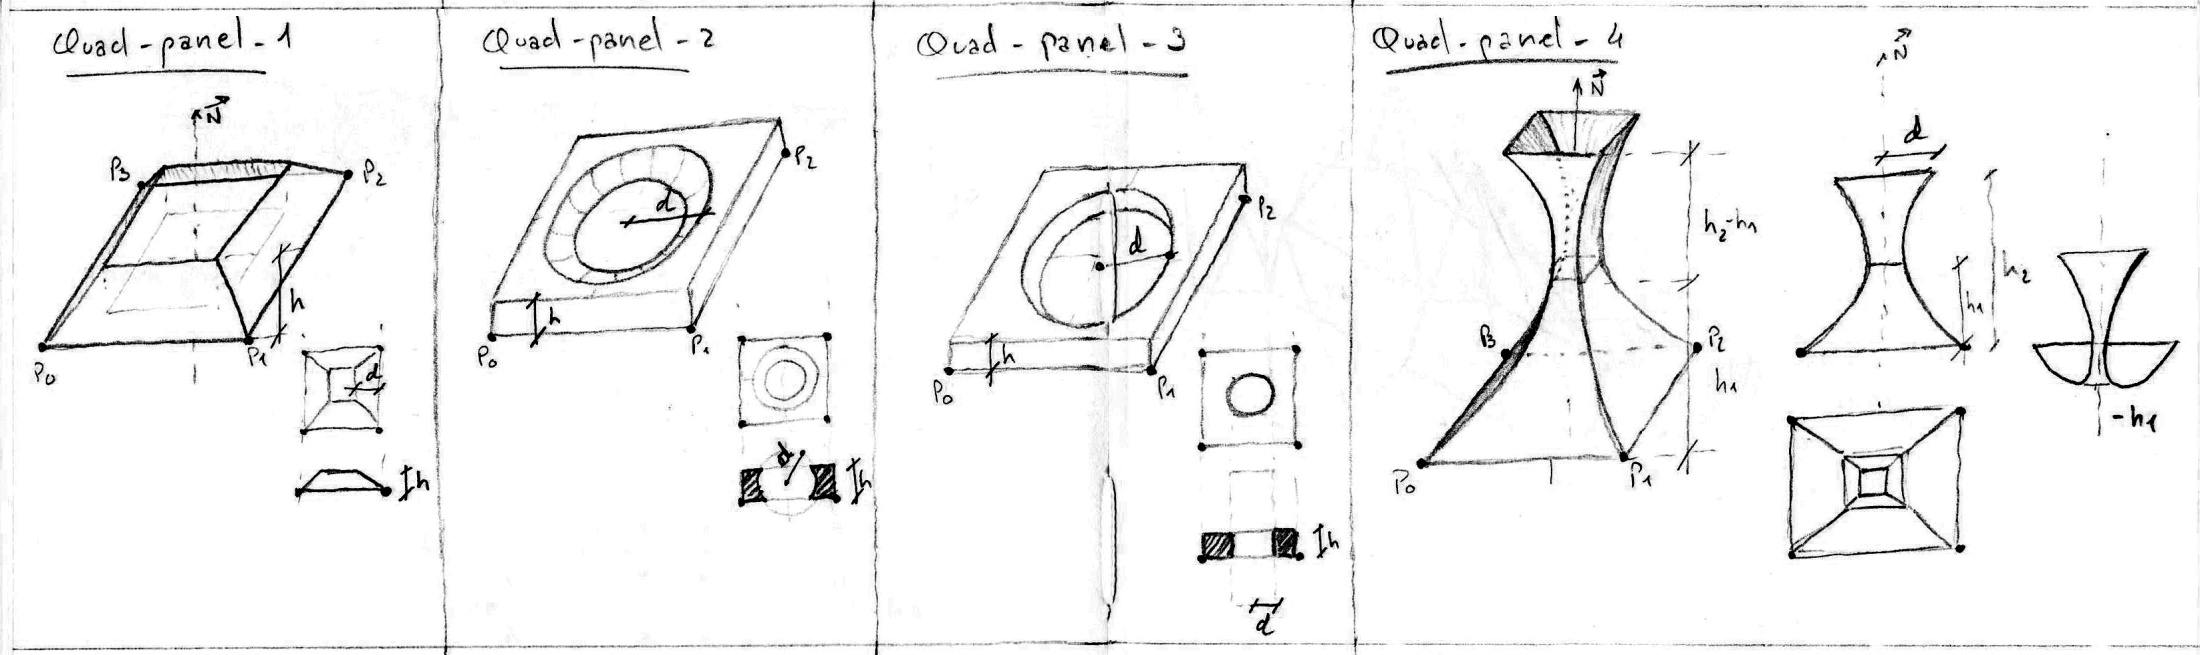
\includegraphics[width=.95\linewidth]{images/real-sketch}
  \caption{Sketches made during architectural design phase}
  \label{fig:sketch-fig}
\end{subfigure}%
\begin{subfigure}{.4\textwidth}
  \centering
  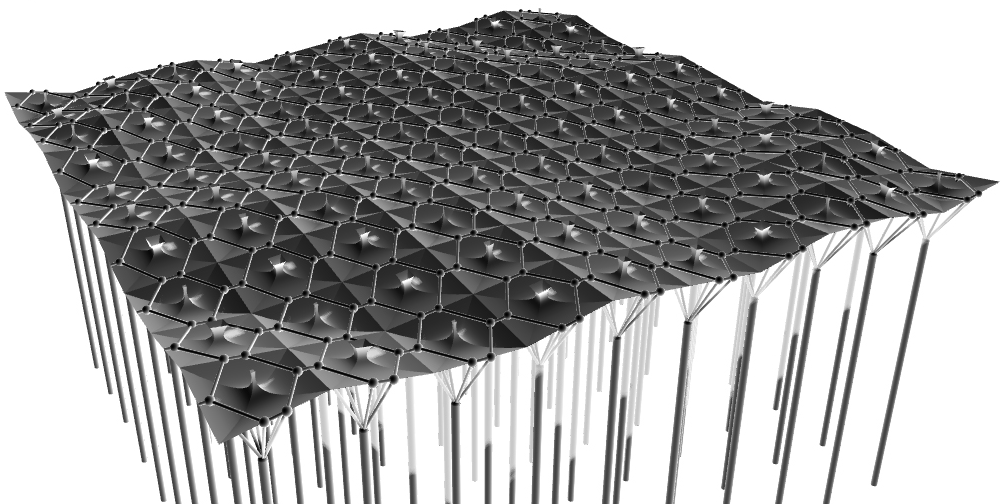
\includegraphics[width=1.0\linewidth]{images/real-sketch-result1}
  \caption{An application of the objects modeled previously in an architectural model}
  \label{fig:sketch-fig-result}
\end{subfigure}
\caption{Typical example showing the importance of design phase in the geometric model conception}
\label{fig:sketch-using}
\end{figure}

In the context of \gls{gd} methods these sketches becomes even more relevant because they serve as basis for implementing the program. By definition of \gls{gd} method it formally defines a description of an architectural model~\citep{mccormack2004generative}. In this way, while the code define the geometric object textually, the sketch define the geometric object visually. Consequently, it is fundamental during the development of the program but it is also a rich source for documenting the program. Different from the typical programs in software engineering which is purely textual and may express concepts that is difficult or even impossible to represent graphically, the program in \gls{gd} has this particularity of being able to represent its concepts through sketches or diagrams.

Surely sketches and diagrams are a suitable medium to express complex ideas. More than that, the architect frequently uses sketches because it helps him to reason about the conception of the design itself. And the \gls{gd} approach does not change this fact, on the contrary the use of sketch to illustrate program's components become even more popular, because it turns programming into a more  concrete and noticeable task, giving special clues for novice programmers. At the end of writing the program, all architect's decisions and insightful design, applied to construct the final program, are encapsulated in these sketches. As a result, these
sketches are also an essential artifact to comprehend the program specially after its release. 

For example consider the Figure~\ref{fig:chairseat} (reference here) that portrays a real example of a chair seat which was parametrically modeled. Even the less curious reader will wonder to know what each symbol of this image means. Some of them are more obvious than others, for instance the angles and the differences between them, however this diagram has its meaning embedded in problem context. It means that, those symbols in the image are variables which were created purposely to solve the problem of creating different shape of seats by varying the variable values. So the sketch proposes a parametric model of chair seats, additionally it contextualizes the meaning of each variable. Using this example the architect is able to create a suitable \gls{gd} method that creates this chair seat, however the \gls{gd} approach is not so straightforward as it seems to be. 

\begin{figure}[!htbp]
%\vspace{-5pt}
  \centering
  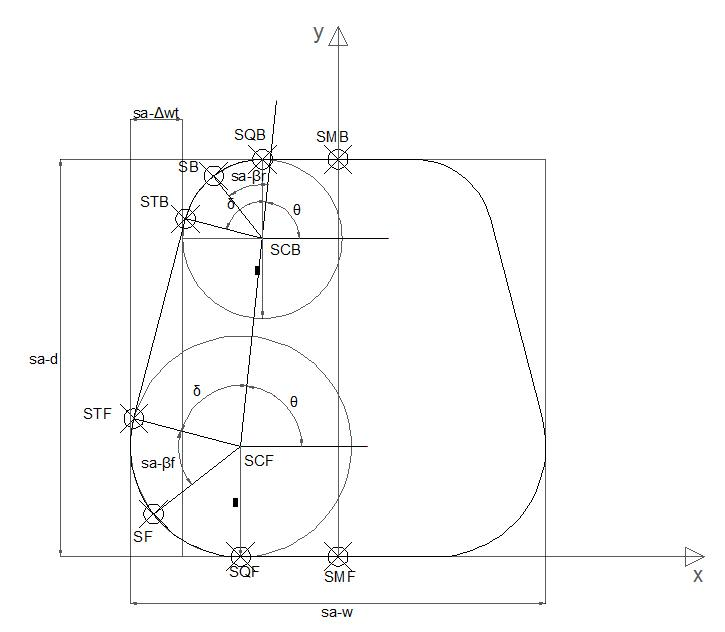
\includegraphics[width=0.5\textwidth]{images/seat}
    %\vspace{-15pt}
    \caption{A real sketch of a chair seat. In this sketch the seat is parametrized with some geometric variables. Some of them are intuitively noticeable, e.g. the angle symbols $\delta$, $\theta$, and $\beta$, but rest of them are not, because they have its meaning embedded in the problem context}
    %\vspace{-5pt}  
  \label{fig:chairseat}
\end{figure}

The problem with the \gls{gd} methods is that when a geometric model is rewritten in a programming language all visual information that perhaps its diagrams show is lost. For example the diagram in Figure~\ref{fig:chairseat} would be written using the following function signature: \\

\begin{minipage}[c]{.8\textwidth}
\texttt{/* this function creates a chair seat */} \\
\texttt{make-seat(SMF, SCF, SCB, sa-d, sa-w, sa-$\Delta$wt, sa-$\beta$r, sa-$\beta$f) \{} \\
\texttt{\hphantom{...} // the function body} \\
\qquad \texttt{\hphantom{...} ...} \\
\texttt{\}}
\end{minipage} \\

For the architect who did the sketch and implemented the code this function may appear simple enough to be understood. For people who will get this code posteriorly this kind of functions could give a headache nonetheless. Actually in the architect's mind all these functions parameters make sense, because they all are part of the design and the sketch can prove it. The problem is that the sketch is not delivered with the program, moreover the program is usually delivered without any documentation or may have useless comments as that one in the example. Consequently, it negatively affects people who need to use this program, because without documentation they cannot understand the program well enough to use, or modify it, affecting the entire \gls{gd} community. 

\section{Sketch-program correlation tool}

As discussed in the previous section, the lack of documentation in \gls{gd} programs affects negatively its users. In fact this problem is beyond \gls{gd} area, it affects also the field of software engineering. In this field, there were attempts to improve this problem by improving the quality of program documentation, most prominently, \textit{literate programming}~\citep{knuth1984literate}. This work proposed a programming paradigm that promoted the fact that program are written for people first and foremost, and that documentation should be emphasized just as much as code. Unfortunately, these attempts did not reach the intended goals, mainly because writing good documentation takes considerable amount of time and effort.

A more recent work~\citep{learnableProg} suggested that the programming environment should minimize this tough work required to write documentation by providing the documentation programmers need when they are reading the code. In this work, Victor outlines the following idea:

\blockquote{The environment is responsible for making meaning transparent. The environment must enable the reader to effortlessly read the program, to decode the code, so he can concentrate on genuine programming concepts~\citep{learnableProg}}

Figure~\ref{fig:victor-ex} shows a prototype, presented with this work, that demonstrates how the environment can improve the program readability. The code in prototype is written in Processing language~\citep{Reas2006} (on the left) and it  sets the environment color to green and creates two geometric objects: a circle and rectangle (on the right) by using the Processing functions: \texttt{fill, ellipse and rect}. This programming environment make meaning of each element of the code transparent, by providing labels on mouse-over. For example, the reader will know that the fourth parameter of function \texttt{rect} will change the height of the rectangle when he points to that parameter. And he can also point to every element of this code to get its meaning, so even before he makes any change in this code he will know exactly what the code is doing.     

\begin{figure}[!htbp]
%\vspace{-5pt}
  \centering
  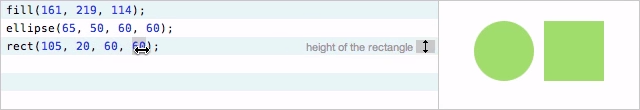
\includegraphics[width=.7\textwidth]{images/victor-example}
    %\vspace{-15pt}
    \caption{A programming environment that helps in the program readability. On the right, is a sample of code, written in Processing language, that creates a green circle and rectangle. On the right, is the produced result of this code. Each element of this program, including the functions and its arguments, are labeled so when user point the mouse over an element its label appears on the editor.}
    %\vspace{-5pt}  
  \label{fig:victor-ex}
\end{figure}

Labeling the program elements on mouse-over indeed make the program meaning more explicit, but this technique does not replace the need of a proper documentation. The main problem with this approach is that these labeled functions already exist in Processing, so this feature is more intended to avoid unnecessary searches on the Processing manual, than alternatively provides a way to document the program. For any user defined function this feature will not work, consequently the programmer must take considerable amount of time and effort to create its own documentation.

The reality in architecture is quite different form that in software engineering: it is part of the design process to produce documentation in the form of sketches. This means that it is not necessary to write huge amounts of textual documentation to explain a \gls{gd} program. We only need to annotate the already existing sketches and combine them with the program, thus providing visual explanations of what the program is supposed to do.

In Figure~\ref{fig:sc-tool} I propose the \textit{sketch-program correlation tool} that shows how sketches and code can be combined to provide useful documentation for the programmer by using the sketches made in a early phase of program design. This example illustrates a function that draws an arrow giving the base point $P$, the direction $\alpha$, the height $\rho$, and the width $\beta$ and size $\sigma$ of the arrow tip. This information is all condensed in the sketch, maybe even more precise. So the idea of this tools is to take advantage of this fact by pointing out what is the meaning of each function parameter, found in the code, in the context of the sketch (and vice versa). In this way, when the user has the mouse over a function parameter he immediately sees what that parameter correspond in the sketch, and  the inverse is also valid: when he moves the mouse over a symbol in the image he immediately see its meaning in the code. That helps him to create a mental model of the program even before to change it.

\begin{figure}[!htbp]
%\vspace{-5pt}
  \centering
  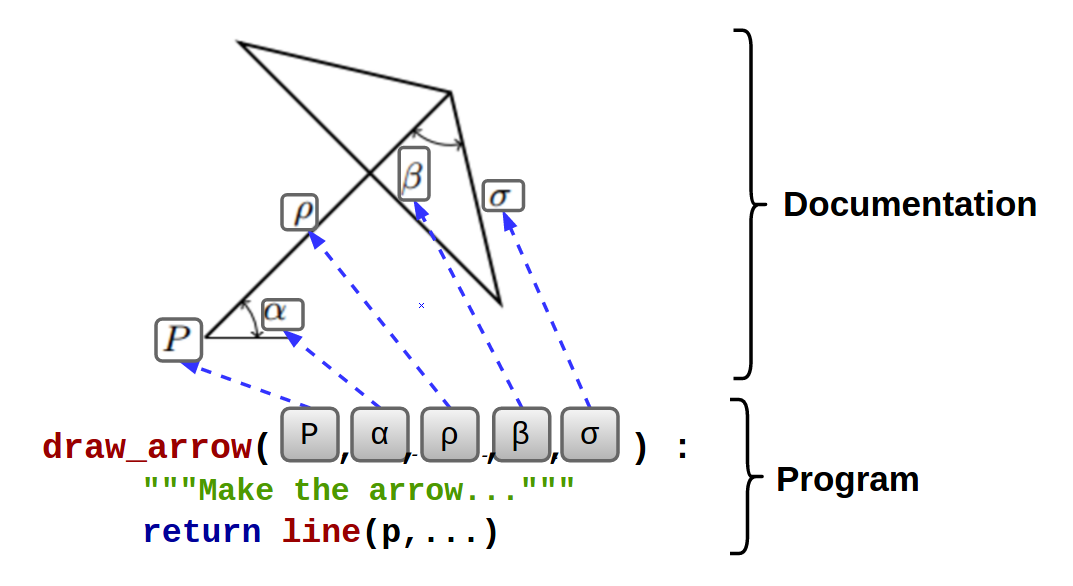
\includegraphics[width=0.5\textwidth]{images/proposed-sc-tool}
    %\vspace{-15pt}
    \caption{\textit{Sketch-program correlation tool} showing how to combine fragments of the program with sketches. In this example all the function parameters has a correspondent symbol in the sketch that illustrate its meaning}
    %\vspace{-5pt}  
  \label{fig:sc-tool}
\end{figure}

As demonstrated in early works, the underline principle behind this tool can in fact helps in the program readability, consequently helping in the overall process of program comprehensibility. However implement this tool in the current environments for \gls{gd} is undoubtedly a hard  challenge, due the absence of certain capabilities required for implementing this kind of tool considering the current state of \gls{gd} environments.

Perhaps the first challenge imposed by this tool, is in how to include images in the code editor. It seems a trivial problem, however the possibility to insert a simple image in the code editor is unsupportable for at least the majority of code editors. Specially in \gls{gd} where the environments used for textual languages generally only support rows of plain text. Until the time we are not aware of any other code editors that provide such a capability, in exception of Rosetta tool~\citep{lopes2011portable} that provides an enhanced code editor that supports images and other media-rich elements, by using DrRacket~\citep{findler2002drscheme} as its code editor.

A inherent concern in the fact of supporting images in the code editor is on how to store it. The strategy used by DrRacket, is to serialize the image and store it in ascii-encoded binary format. The problem of this strategy is that once the programmer inserts an image in his code and save it, he will not be able to change its code again using other text editor. So this method does not provide any backwards-compatibility with other text editors potentially useful to write programs. As a result, it makes difficult, or even impossible, the portability of the program among those different text editors.

I propose another approach to this problem that assures backwards-compatability. The first step is to define a standard annotation that will be used to include the image, similarly to the Java doc annotation. Then requires the use of that annotation upon an event of image insertion. Thus to include an image the programmer should quote the image with that annotation, as the example depicted in Figure~\ref{fig:inline-image}. As a result, it will be possible for the program environment to distinguish images from source code and proceed to an adequate treatment for those images. 

\begin{figure}[!htbp]
%\vspace{-5pt}
  \centering
  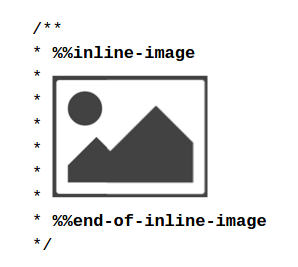
\includegraphics[width=.25\textwidth]{images/inline-image-example}
    %\vspace{-15pt}
    \caption{Example of inline-image annotation.}
    %\vspace{-5pt}  
  \label{fig:inline-image}
\end{figure}

By using this convention, when the programmer save his code all images under that annotation can be stored as a simple source code comment. For example considering the annotation showed in Figure~\ref{fig:inline-image}, the following string would be generated by parsing that annotation:

\begin{center}
\begin{minipage}[c]{.6\textwidth}
\texttt{// \%\%image \$\{USER\_HOME\}/project/sketch1.jpg \%\%}
\end{minipage} \\
\end{center}

The above text is a convection that represents the relative path from where the code editor loaded the image. In this way if the code editor cannot resolve this path and find the image, the code could be showed anyway by displaying just that comment, thus the code can be opened in any text editor. Of course to be able to see the images, programmers must open the code in the text editor capable to interpret that annotations and display the images. 

Other systems, to avoid the problem of incompatibility among editors convert the code into a textual format, for example Barista~\citep{ko2006barista} saves the code in XML. However the presented approach goes further, because it does not impose any language specific requirement, the code is stored as it is (ordinary plain text). So it is up to the code editor to implement suitable methods to show the images.

Nevertheless, an interesting challenge imposed by the sketch-program correlation tool is the automatic recognition of text and symbols in images. Fortunately, this is an old problem which is part of the ancient dream of replicating the human functions by machines, making the machine able to perform tasks like reading. To concertize this dream was realized that information should be readable both to humans and to machine and alternative inputs can not be predefined. As consequence of this probably inputs, an \gls{ocr} system would be necessary for dealing with the problem of recognizing optically processed characters. Optical recognition is performed after the writing or printing has been completed. Therefore the idea of this system is avoiding the traditional way of entering data into a computer through the keyboard by providing a more efficient way for it.

The \gls{ocr} systems rapidly became a prominent field of study that gave substantial incentives for making pattern recognition and image analysis matured fields of science. The very first attempts can actually be found back in 1870~\citep{eikvil1993optical} with the retina scanner which was an image transmission system using a mosaic of photocells. From then, consecutive attempts were made to improve the methods of \gls{ocr} systems, specially by sophisticating the retina scanner and creating OCR machines that became commercially available in the 1950's. Posteriorly, HP as a possible software and/or hardware add-on for HP's line of flatbed scanners, proposed a novel open-source project: Tesseract~\citep{smith2007overview} OCR engine. This project was then sponsored by Google and nowadays is one of the most accurate OCR engine on the market used widely in several web applications.

Clearly the subject of character recognition is extremely extensive and its details are beyond the scope of this dissertation. However, to propose my solution of recognizing automatically text in image, I based on the functionality of the \gls{ocr} engine, namely the Tesseract~\citep{smith2007overview}, that accepts an image file and returns a file with the recognized characters and their respective coordinates on the image. However, the Tesseract is a local application that needs to be installed in the user's computer, or be included as external libraries on the program, which may affect the portability of the application and its use.

To solve this problem I propose the use of \gls{ocr} Web Service, such as\footnote{\texttt{http://www.onlineocr.net/}},\footnote{\texttt{http://www.free-ocr.com/}} that provides the same functionality, because they are build on top of Tesseract, but it defines a more standardized way for integrating the applications using the SOAP or REST. Figure~\ref{fig:sc-tool-arch} shows the architecture of this tool. 


\begin{figure}[!htbp]
%\vspace{-5pt}
  \centering
  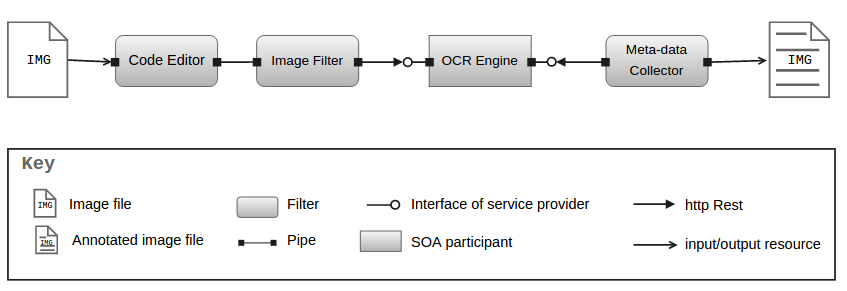
\includegraphics[width=.7\textwidth]{images/sc-tool-architecture}
    %\vspace{-15pt}
    \caption{Data flow view combining two styles: pipe-and-filter style and client-server style.}
    %\vspace{-5pt}  
  \label{fig:sc-tool-arch}
\end{figure}
%!TEX root = ../dissertation.tex

\chapter{Evaluation}
\label{chapter:evaluation}
Evaluation here...

\section{Architecture}
\label{sec:arch}

The problem addressed in this thesis is to design and implement an interactive programming environment for generative design that covers the needs of both beginners and advanced users. Our approach suggests two interactive tools: (1) \textit{sketch-correlation tool}, which correlates sketches with code, as a result it significantly reduces the effort to read the code, and (2) \textit{immediate feedback tool}, which executes the program upon changes, thereby creating an interactive environment to users quickly test their ideas and, eventually, improve program comprehension. The next section shows how these features will work.

\subsection{Experimental results}

An initial prototype was devised to show how code and images can be correlated, as shown in Figure~\ref{fig:images-code}. In this prototype, the meaning of the function and its parameters are transparent, because users can move the mouse over an identifier to figure out its meaning. For example in Figure~\ref{fig:images-code1}, there are two arrows pointing to the identifier \texttt{r}, when we look at the image is easy to see that it represents the radius of the sphere, while the other arrow refers to the location where it is used, i.e. in the \texttt{sphere} function. Especially in this example, the sketch illustrates exactly the function output. The function uses a primitive of Rosetta~\citep{lopes2011portable} (the \texttt{sphere} function) which creates a sphere, given a 3D point and a radius, in the selected \textit{backend}.

\begin{figure}
 %\vspace{-5pt}
        \centering
        \begin{subfigure}{0.5\textwidth}
                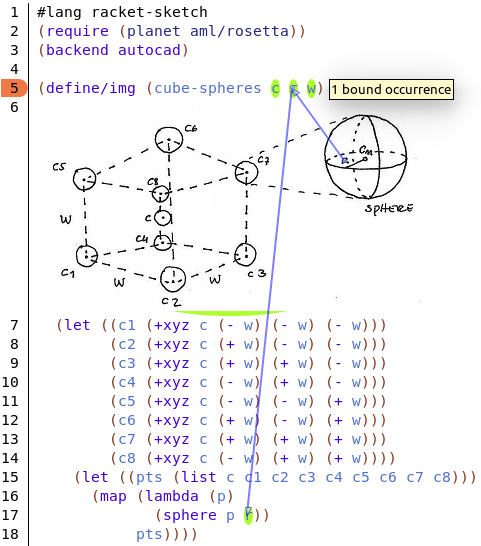
\includegraphics[width=\textwidth]{images/img-code}
                \caption{Searching for ``r'' meaning.}
                \label{fig:images-code1}
        \end{subfigure}%
        ~ %add desired spacing between images, e. g. ~, \quad, \qquad, \hfill etc.
          %(or a blank line to force the subfigure onto a new line)
        \begin{subfigure}{0.5\textwidth}
                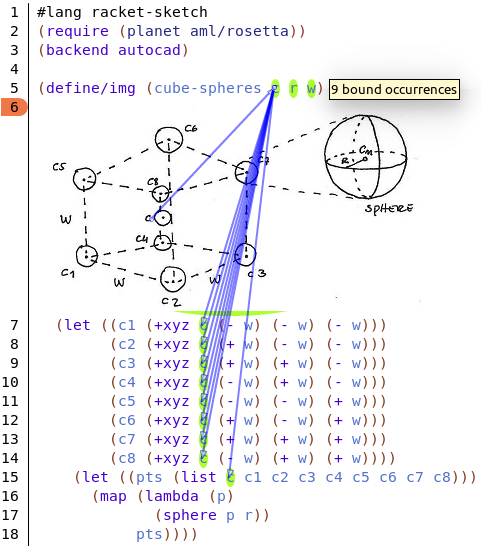
\includegraphics[width=\textwidth]{images/img-code-2}
                \caption{Searching for ``c'' meaning.}
                %\label{}
        \end{subfigure}
        %\vspace{-5pt}
        \caption{Contextualizing the code with image.}
        \label{fig:images-code}
         %\vspace{-10pt}
\end{figure}

\begin{figure}[htb]
 %\vspace{-5pt}
    \centering
        \begin{subfigure}{0.65\textwidth}
                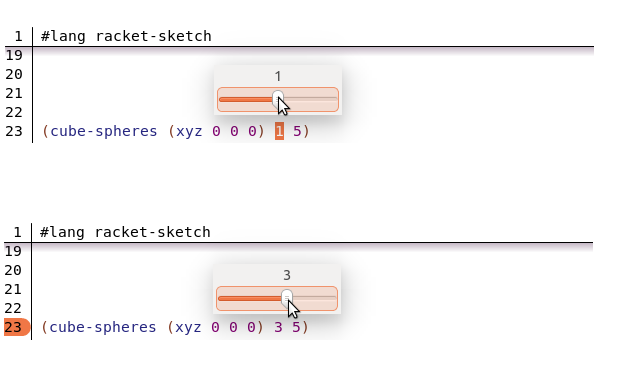
\includegraphics[width=\textwidth]{images/cube}
                \caption{Changing the ``r'' parameter.}
                \label{fig:slider1}
        \end{subfigure}%
        ~ %add desired spacing between images, e. g. ~, \quad, \qquad, \hfill etc.
          %(or a blank line to force the subfigure onto a new line)
        \begin{subfigure}{0.35\textwidth}
                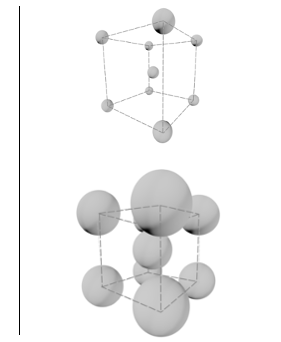
\includegraphics[width=\textwidth]{images/img-cube}
                \caption{The generated models, rendered by AutoCAD.}
                \label{fig:cube}
        \end{subfigure}
        %\vspace{-5pt}
        \caption{Interacting with the \texttt{cube-spheres} function.}
        \label{fig:slider}
 %\vspace{-10pt}
\end{figure}

Using the immediate feedback tool, programmers can test their ideas by quickly experiment them, as the prototype shown in Figure~\ref{fig:slider} which supports this process. In this prototype, the function defined in Figure~\ref{fig:images-code}, i.e. \texttt{cube-spheres}, is being interactively tested. Each change in the slider causes an execution of the program with the new slider value, particularly in this example, it will generate a new geometric model (see Figure~\ref{fig:cube}). As a result, users can confirm that the parameter \texttt{r} is, indeed, the radius of the sphere and it also eliminates the cycle edit-compile-run, allowing fast visualization of changes.  

These features will be built on top of DrRacket~\citep{findler2002drscheme}. In the following sections, we will present relevant properties of DrRacket that justify its choice as the basis of this thesis, as well as the proposed architecture to extend the DrRacket environment.

\subsection{DrRacket Properties}

Like DrRacket, our solution initially will target students, but, eventually, it would be used by anyone who wants to document the code with images or develops a program interactively. Therefore, to implement our solution we choose DrRacket, because it is built in the same principle we search for and has some key qualities:

\begin{itemize}
	\item \textbf{Pedagogic.} DrRacket is a popular environment used in introductory courses for programming languages. The environment is designed to guide the student by catching typical mistakes and explaining them in terms that students understand. It is also useful for professional programmers, due to its sophisticated programming tools, such as the static debugger, and its advanced language features, such as \textit{units} and \textit{mixins}.

	\item \textbf{Sophisticated editor.} DrRacket fully integrates a graphics-enriched editor which supports, in addition to plain text, elements such as images and boxes (with comments, Racket code or XML code). DrRacket also displays these elements appropriately in its read-eval-print loop.

	\item \textbf{Extensible.} The main tools of the DrRacket environment are implemented using the same \gls{api} that is available for extension. For example, the debugger, the syntax checker and the stepper, despite providing different functionalities, are implemented on top of the same \gls{api}.
\end{itemize}

Moreover, DrRacket helps programmers to understand the syntactic and lexical structure of their programs. DrRacket provides a syntax checker that annotates a syntactically correct program in five categories: the primitives, keywords, bound variables, free variables, and constants. When the programmer moves the mouse over an annotated identifier, the syntax checker displays arrows that point from bound identifiers to their binding occurrence, and vice-versa (see Figure~\ref{fig:images-code}). However, the syntax checker ignores the category of comments, including its visual elements such as the images, as a result these elements are uncorrelated with the program's structures and behavior.

In the next section, we propose an architecture which aims to address the above issue as well as proposes a solution for the immediate feedback tool.

\subsection{Proposed Architecture}

Figure~\ref{fig:solution} presents a publish-subscribe view of the proposed features. There are two different interactions in this architecture, the first presented by a publish-subscribe and the second by a client-server.

\begin{enumerate}
	\item The main functionality of the proposed environment is made through a publish-subscribe interaction. The \texttt{DrRacket \gls{ui} event manager} acts as an event bus for user-interface events (such as button clicks). From this event bus we subscribe only the \gls{ui} events which are relevant to our system, defining which components will handle them. It is done at load time when the event manager reads the \textit{plugin} configuration file (\texttt{info} file). When users are working on the editor, an \gls{ui} event is generated and dispatched via implicit invocation to the action handler objects that subscribe to that event.

	\item The client-server interaction is only needed to support the correlation between images and code. We assume that the images, inserted in the editor, will be associate to a single function and will contain the same identifiers defined by its associated function parameters (as shown the handmade sketch in Figure~\ref{fig:images-code}). Then, the manuscript symbols present in the image (e.g. the parameters ``c'',``r'', and ``w''), will be parsed using an \gls{ocr} engine. This engine usually gets an image and returns a text file containing a symbol table with the parsed symbols and its respective coordinates. We expect the \gls{ocr} engine to act as an external service that identifies those symbols, thereby in our architecture the \texttt{symbol identifier} component calls this service to handle the recognition of symbols in the image.
\end{enumerate}

\begin{figure}[htb]
 %\vspace{-15pt}
	\centering
	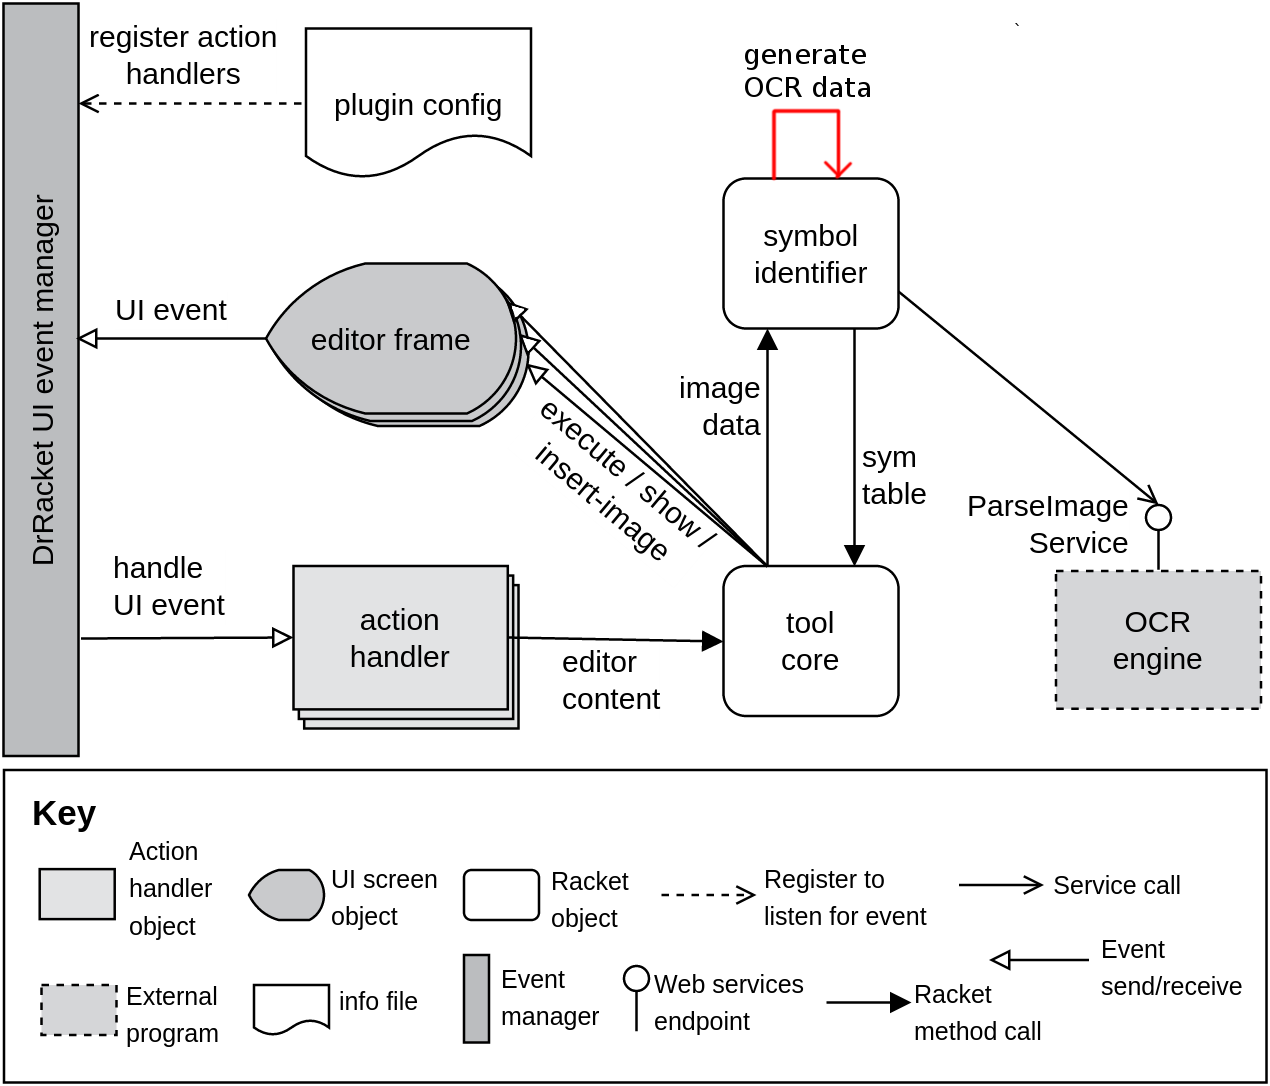
\includegraphics[scale=0.19]{images/solution}
	%\vspace{-5pt}
	\caption{Diagram for a publish subscribe view of the proposed architecture.}
	\label{fig:solution}
 %\vspace{-10pt}
\end{figure}

The \texttt{tool core} component, in Figure~\ref{fig:solution}, will receive, at least, three kinds of DrRacket events. For each of these events, we will change the programming environment based on the following desired action:

\begin{itemize}
	\item \texttt{on-change:} when DrRacket detects that the editor has been modified, it sends the contents of the editor over to action handlers.	The action handler, in this case, it the \texttt{online expansion handler} where the code is expanded. \textit{Desired action}: sends an \texttt{execute} event to the editor frame, if the action handler expanded the code successfully. 

	\item \texttt{on-paint:} this event is sent just before and just after every element is displayed in the editor. Handling this event provides a way to add arbitrary graphics to the editor display. \textit{Desired action}: sends a \texttt{show} event to the editor frame, to display a slider widget when the user moves the mouse over a literal.

	\item \texttt{on-new-image-snip:} this event is sent when an image is inserted in the editor. The default implementation creates an image snip which is an object with the image information, such as path and format. \textit{Desired action}: sends an \texttt{insert-image} event to the editor frame, before to get the image and send it to the \gls{ocr} engine to recognize its symbols and respective coordinates (x, y). Then, it returns a subclass of image snip, containing this extra information.
\end{itemize}

Finally, to correlate the image-snip, created above, with the function parameters we will use a syntactic transformer, i.e. macro. The macro will add a new syntax form into the language grammar, allowing an image to be used as a comment. Very similar to Lisper's comment, the macro will add a new rule in the grammar, where an image is between a function declaration and a function body (see the macro \texttt{define/images} in figure~\ref{fig:images-code}). The image will be ignored, but in background, our macro expansion will add into the function body new occurrences of the function parameters. As a result, the DrRacket syntax checker will mark these free variables and will be able to recognize bound occurrences and point to them inside an image.

\section{Evaluation}
\label{sec:eval}

The evaluation of the proposed architecture will be performed experimentally, building a prototype. The prototype will serve to test the proposed ideas and to evaluate them. To evaluate the prototype, we will use the Rosetta~\citep{lopes2011portable} generative design tool as a case study. As Rosetta is used by architects, and designer, we will receive real feedback from the target users. In this way, we can evaluate if our programming environment helps their target users to design programs.

Furthermore, to evaluate our proposal we plan to use the following evaluation metrics.

\begin{itemize}
\item \textbf{Correctness.} To assess the quality of our system we plan to test, individually, each proposed feature with a specific test case scenario, for example using the slider widget to explore the result of a parametric function and inserting different kinds of images and check if the image is well correlated with the function parameters. 

\item \textbf{Security.} Among others qualities, security is an important concern in a live environment where the code is executed instantly. In our case, the code is executed locally, however while the users are using the live code mode they can create dangerous constructs such as \texttt{eval}, \texttt{exec} and \texttt{file I/O} which can damage the operating system. On the other hand, in this mode it is possible to block the environment with a simple ``while true'' expression. To avoid these problems, we plan to implement sandboxing, similar to PythonTutor~\citep{GuoSIGCSE2013}, and design specific tests to test this feature.

\item \textbf{Performance.} The performance of our system should scale for the generative design programs. The Rosetta tool will give us different \textit{backends} to test the performance of our interactive tool. In fact, to be an interactive tool, the response for an event should be quick ($\sim$50ms). It imposes restrict requirements for the CADs tools, because these tools were designed for the speed of human operation, consequently they are the performance bottleneck. This issue forces us to establish a limit which this tool will be tested, thus we will compare this limit against other similar systems.

\item \textbf{Comparison with other systems.} We can only claim that our solution is somehow better than the other, if we compare them. Therefore, we plan to compare our system with the existing programming environments in generative design, particularly the visual environments, such as Grasshopper. Between these systems, the performance limit, stated above, will be our reference of comparison.
\end{itemize}
%!TEX root = ../dissertation.tex

\chapter{Conclusion}
\label{chapter:conclusion}
Conclusion here...



\bibliographystyle{ieeetr}
\addcontentsline{toc}{chapter}{Bibliography}
\bibliography{bibliography/dissertation}

% Appendix
\appendix
%!TEX root = ../dissertation.tex

% Entry point for chapters
% In this file you define the order
% in which the chapters are included

\setlength{\parindent}{2em}
% Configure the space between paragraphs
\setlength{\parskip}{1.0em}
%\setstretch{1.5} 

% Chapters
%!TEX root = ../dissertation.tex

\chapter{Introduction}
\label{chapter:introduction}
Your introduction here...\\

A demonstration of how to use acronyms and glossary:

A \gls{MSc} entry.

Second use: \gls{IST}.

Plurals: \glspl{MSc}.

A citation example \cite{nobody}

%!TEX root = ../dissertation.tex

\chapter{Background}
\label{chapter:generativeDesign}

In this chapter, I introduce the context and background for subsequent chapters. The first part addresses fundamentals concerning on teaching programming to novice students, and the relationship between programming and the related issues. The second part describes the typical components of software development environments used in Architecture, highlights the different types of available tools, and introduces the challenges of enabling programming on these environments.

\section{A Programming Framework}

Programming used to be taught mainly in computer engineering courses. In recent years the demand for programmers and student interest in programming have grown rapidly, and programming have become a subject increasingly important in several areas of study. Learning to program is hard however. Novice programmers suffer from wide range of difficulties and deficits. It is generally accepted that it takes about 10 years of experience to turn a novice into an expert programmer (Winslow, 1996).

Why programming is such a hard subject to learn? What resources and
processes are involved in creating or understanding a program? Since the 1970s there has been an interest in questions such as these, and in programming as a cognitive process. The literature relating to such topics is extensive, and it is divided into two main categories: those with a software engineering perspective, and those with a psychological/educational perspective.

Learning to program is usually addressed from a psychological/educational perspective, however our interest is in novices and in how the programming environment can provide adequate tools to support the initial development of individual programming skills. Early learning should of course include the basics of good software engineering practice such as comprehend the program structures, documenting the program, testing and debug among others.

Before propose any kind of feature it is first necessary to research what are the main challenges in this area. In fact programming is beyond coding, it involves knowledge about computer, programming language, programming tools and resources, and ideally theory and formal methods. As important as knowledge is the way knowledge is used and applied, also known as strategy. Writing a program involves also maintaining many different kinds of ‘mental model’ which is the way programmers comprehend its programs.

\begin{table}[!htbp]
\centering
\begin{tabular}{@{}lllll@{}}
\cmidrule(r){1-4}
 & \textbf{Design} & \textbf{Generation} & \textbf{Evaluation} &  \\ \cmidrule(r){1-4}
\textbf{Knowledge of} & \begin{tabular}[c]{@{}l@{}}planning methods,\\ algorithm design,\\ formal methods\end{tabular} & \begin{tabular}[c]{@{}l@{}}language, libraries,\\ environment / tools\end{tabular} & \begin{tabular}[c]{@{}l@{}}debugging tools\\ and methods\end{tabular} &  \\ \cmidrule(r){1-4}
\textbf{Strategies for} & \begin{tabular}[c]{@{}l@{}}planning,\\ problem solving,\\ designing algorithms\end{tabular} & \begin{tabular}[c]{@{}l@{}}implementing\\ algorithms, coding,\\ accessing knowledge\end{tabular} & \begin{tabular}[c]{@{}l@{}}testing, debugging,\\ tracking / tracing,\\ repair\end{tabular} &  \\ \cmidrule(r){1-4}
\textbf{Models of} & \begin{tabular}[c]{@{}l@{}}problem domain,\\ notional machine\end{tabular} & desired program & actual program &  \\ \cmidrule(r){1-4}
\end{tabular}
\caption{My caption}
\label{tab:framework}
\end{table}


The Table~\ref{tab:framework} (adapted from~\cite{robins2003learning}) proposes a programming framework that makes explicit the implied relationships between many of the issues found by novice programming. It highlights the relationship between the individual attributes (discussed above) with the program phases namely design, generation and evaluation. Undoubtedly the three phases are important, however the design phase is the most important because it is the basis of program understanding

Rist notes: There is considerable evidence in the empirical study of programming that the plan is the basic cognitive chunk used in program design and understanding.

\section{Coding in Architecture}

\section{Programming Languages \& Programming Environments}

%TEX root = ../dissertation.tex

\iffalse \bibliography{bibliography/dissertation} \fi


\chapter{Related Work}
\label{chapter:relatedWork}

In this chapter, I summarize related research on development environments and programming languages. Work presented here focuses on the programming tools used in different contexts and environments, whereas technical aspects and software architecture are separately discussed in Chapter x. Also, this chapter includes work on improvements to code intelligence features such as representation of code.

My work lies at the intersection of two main research areas: \gls{se} and \gls{gd}, consequently the related work present the recent advances in both of these areas.

\section{Programming System}
\label{sec:ps}
A \textit{programming system} has two fundamental parts: the \textit{programming language} that users should know in order to create a program, and the \textit{programming environment} that is used to write and test programs. Undoubtedly, both parts are equally important to build a program and understand it. However the boundaries between these parts can be blurred, for this reason the related work goes beyond programming environments including also programming languages and their design aspects. 

Based on prior surveys of novice programming environments~\citep{kelleher2005lowering}, in the following sections I divide the programming systems in three categories: (\ref{sec:gs}) general-purpose systems; proposed for building complex software, (\ref{sec:ts}) teaching systems; proposed to teach programming, and (\ref{sec:es}) empowering systems; proposed to build programs tailored to specific needs. In each category, we focus on the tools provided by the programming environment.
%%%
\section{General-purpose systems}
\label{sec:gs}

The systems in this category are built to support all, or at least a substantial part, of the software development process. To this end, these systems suggest an \gls{ide} that aims to support the entire development process by grouping in a single environment all necessary tools.

In this section we describe, in detail, two relevant \glspl{ide}: Eclipse~(open-source)~\citep{carlson2005eclipse} and LightTable (open-source)\footnote{\label{fnote:lt}\texttt{http://lighttable.com/}}. Other popular \glspl{ide} include NetBeans~(open-source)~\citep{boudreau2002netbeans}, Microsoft's Visual Studio~(commercial)~\citep{guckenheimer2006software}, or Apple's Xcode~(free but closed-source)\footnote{\texttt{https://developer.apple.com/xcode/}}. Some \glspl{ide} (eg., Visual Studio or Xcode) primarily target the environment and ecosystem of the manufacturer's own programming languages.  The following study use those \glspl{ide} for the sake of comparison, because they provide similar features to Eclipse or LightTable.

%%%%%%%%%%%%%%%%%%%%%%%%%%%%%%%%%%%%%%%%%%%%%%%%%%%%%%%%%%%%%%%%%%%%%%%%%%%%%%%%%%%%%%%%%%%%%%%%%%%%%%%%%
\subsection{Eclipse} 
\label{subsec:eclipse}
Eclipse~(Figure \ref{fig:eclipse}), a project initiated in 2001 and promoted by a consortium of industry leaders~\citep{carlson2005eclipse}, is a widely used open-source \gls{ide}. It is used mainly by Java developers, although it supports other programming languages such as C, C++ and JavaScript. As showed in~\citep{murphy2006java}, the commonly cited reasons for using Eclipse include rich Java development tools support and a \textit{plugin} architecture, the Eclipse Platform~\citep{DesRivieres2004}, that allows tight integration of third-party functionality.

The Eclipse platform~\citep{DesRivieres2004} has a common architecture among the \glspl{ide} presented in this category. This architecture is characterized by two main components, the \textit{plugin} which is the smallest unit of functionality that can be developed and delivered separately, and the platform runtime which will discover and connect the \textit{plugins} to the platform itself. As a result, the platform integrates several tools that are used in distinct phases of the software development process. Figure~\ref{fig:eclipse} shows the \gls{ide} opened in the Java perspective, suggesting a quick fix for the error.

\begin{figure}[!htbp]
%\vspace{-5pt}
  \centering
  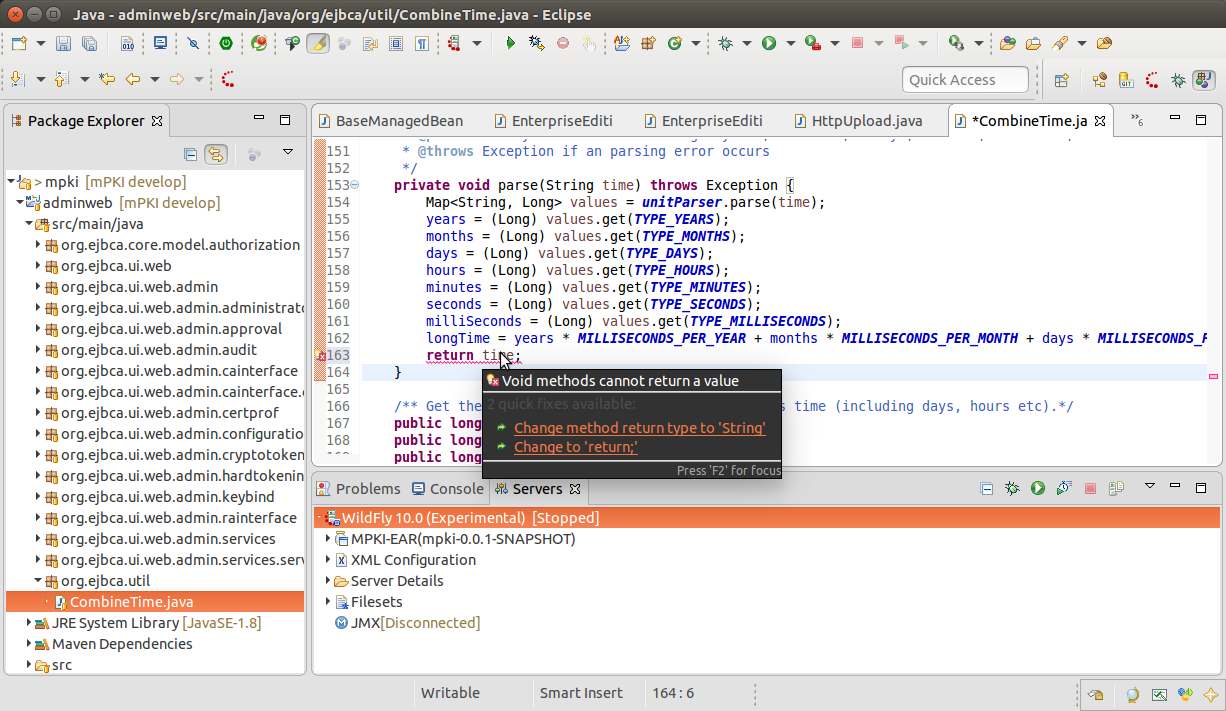
\includegraphics[width=1.0\textwidth]{images/eclipse-2}
    %\vspace{-15pt}
    \caption{Eclipse Integrated Development Environment showing Java perspective}
    %\vspace{-5pt}  
  \label{fig:eclipse}
\end{figure} 

Programming is a laborious task, even worse with verbose programming language such as Java. For example, while the developer is writing code he usually makes some errors, from lexical errors to semantic errors, that he will only detect after compiling the code. So, he needs to stop his main task to compile the code, and eventually debug it. This edit-compile-debug cycle is extremely unproductive and naturally undesired in an industry environment. 

To prevent this problem a common feature among \glspl{ide} is the instant feedback. This feature aims to anticipate the state of the current program by indicating eventual errors or mistakes made during development. To provide instant feedback Eclipse is constantly compiling the code in background, and giving immediate feedback for the developer in form of syntax highlighting, code completion suggestions, and indications of problems associated with various locations in a source file. 

In the literature a similar concept, known as \textit{liveness}~\citep{alpern1985defining}, referring to the ability to modify a running program. There are several levels of liveness and this kind of tool represent the first level~\citep{tanimoto2013perspective}. The tools in the first levels respond after a programmer action, while the tools at the last level not only run the program and respond immediately, but also predict the next programmer action. Having those tools in a \gls{ide} would be the ideal, however it is far from the reality of nowadays \glspl{ide} tools. 

Before to idealize any new features is important to highlight the drawbacks of the existent ones. Eclipse as the other similar \glspl{ide} share some problems, as for instance:

\begin{itemize}
	\item They are incidentally complex. There is an immense amount of work to be done in those \glspl{ide} that is indirectly related to the real problem itself. For example, until the programmer gets a simple program to run, he needs to install and configure a set of necessary software, and he needs also to configure the development environment. This is a tiresome and time consuming task that adds an extra complexity into programming which is already a complex subject.

	\item Program execution is difficult to observe, such that the only way to see how the program executes is by a stepwise debugger. This forces the programmer to stop the program and look at a line in a single instant of time. Consequently, the programmer cannot see how his program is executing, nor how his changes affect its execution.
\end{itemize}

The complexity of install and configure an \gls{ide} negatively affects the programming language itself, because users are more interested in the capabilities of the language than the \gls{ide}. To overcome this problem, recent programming languages, such as Rust~\citep{matsakis2014rust}, propose an \gls{ide} on the web browser\footnote{\texttt{https://play.rust-lang.org/}}. So users can write programs and use the language without any previous configuration. However this web environment is suitable only for tutorials and small examples, otherwise to have full access to the language users must pay the price to install and configure the language and the \gls{ide}.

%%%%%%%%%%%%%%%%%%%%%%%%%%%%%%%%%%%%%%%%%%%%%%%%%%%%%%%%%%%%%%%%%%%%%%%%%%%%%%%%%%%%%%%%%%%%%%%%%%%%%%%%%
\subsection{LightTable}
\label{subsec:lighttable}
LightTable$^{\ref{fnote:lt}}$ is a successfully crowd-funded project that indicates that instant feedback attracts wide interest beyond the research community. This is further supported by Apple, who have recently integrated a feature called Playgrounds into the Xcode \gls{ide}. Playgrounds are enabled by Apple's new programming language Swift\footnote{\texttt{https://developer.apple.com/swift/}} and allow developers to edit code and immediately see the results of execution.

LightTable is based on Bret Victor ideas which in his influential work~\citep{inventingPrin,learnableProg} pointed out serious problems with the current environments and showed, using prototypes, how the environment can help to address those problems. LighTable is proposed to build web application and to support this process, it provides, at least, two useful features: (1) live execution feedback, that executes the program on every change showing the program flow, and (2) the organization of code in tables, enabling quick access to the program documentation.

\begin{figure}[!htbp]
%\vspace{-10pt}
  \centering
  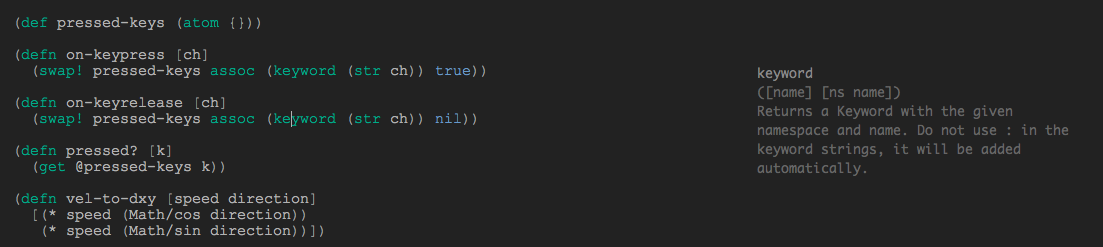
\includegraphics[width=1.0\textwidth]{images/lt2}
    %\vspace{-15pt}
    \caption{LighTable interactive development environment}
    %\vspace{-10pt}  
  \label{fig:lt}
\end{figure} 

LightTable was initially implemented in Clojure\footnote{\texttt{https://clojure.org/}} a general-purpose programming language dialect of Lisp that runs on top of \gls{jvm}. Progressively the code initially written in Clojure was rewritten in ClojureScript\footnote{\texttt{http://clojure.org/clojurescript}}, a script language that uses Clojure compiler which targets JavaScript. Due to its implementation, in LightTable adding a new \gls{ui} element into the programming environment or changing an existing one is doable in a short amount of time, contrary to other \glspl{ide}, such as Eclipse~\citep{carlson2005eclipse}, where an equivalent change requires considerable amounts of time. 

The program documentation in LightTable is quickly accessed by a lateral tab, where primitive functions of Clojure and ClojureScript can be consulted. This documentation is a textual description of the function parameters, the type of return, and some usage suggestions. While looking at a program, it is helpful to have the documentation of strange primitives, such as the \texttt{keyword} function shown in Figure~\ref{fig:lt}, however non-primitive functions are still undocumented. 

\begin{wrapfigure}{r}{0.3\textwidth}
  %\vspace{-30pt}
  \begin{center}
    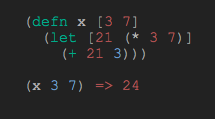
\includegraphics[width=0.3\textwidth]{images/eval-close}
  \end{center}
  %\vspace{-15pt}
 \caption{LightTable real-time debugger.}  
  %\vspace{-20pt}
    \label{fig:lt2}
\end{wrapfigure}

On the other hand, programmers are encouraged to understand new functions by seeing how the values of a function call flow through it. This feature is based on the old idea of Lisp environments: the \gls{repl} which is a prompt used to try out expressions of the language without having to run all the code. This approach goes further by using reflection mechanisms to trace the function call values and shows them filled in the function template (as shown in Figure~\ref{fig:lt2} the flow of values produced by calling \texttt{(x 3 7)}).

The real-timer debugger is an interactive way to debug the code and understand the program flow. Using this feature in an arbitrarily complex program (a program with more than 30 functions) is, however, worthless, because, all the programmer sees is a replica of his functions filled with numbers. It is a poor representation of flow which forces the programmer to spend as much effort with this feature as without it. For this reason, other systems, described in this report, represent the program flow using graphs which are more appropriate in some cases, for example, to show error occurrences in the source code.

Despite providing some tools which are state of the art, LightTable remains in an experimental phase. It has serious limitations to identify and clearly present the errors in the source code. This problem is, mainly, related with the Clojure compiler which loses significant \textit{metadata} between conversions. Consequently, programmers can spend more time and effort to find a bug using LighTable, than using the other \glspl{ide}, such as Eclipse.
%%%%%%%%%%%%%%%%%%%%%%%%%%%%%%%%%%%%%%%%%%%%%%%%%%%%%%%%%%%%%%%%%%%%%%%%%%%%%%%%%%%%%%%%%%%%%%%%%%%%%%%%%
\section{Teaching systems}
\label{sec:ts}
Unlike the previous systems, teaching systems are designed with the goal of helping people learning to program. Most of the systems in this category provide simple programming tools that expose the novice programmers some of the fundamental aspects of the programming process. After acquiring experience with a teaching system, students are expected to move to a more general-purpose environment. 

%%%%%%%%%%%%%%%%%%%%%%%%%%%%%%%%%%%%%%%%%%%%%%%%%%%%%%%%%%%%%%%%%%%%%%%%%%%%%%%%%%%%%%%%%%%%%%%%%%%%%%%%%
\subsection{LOGO} 
\label{subsec:logo}
LOGO~\citep{papert1980mindstorms} is a programming language and environment intended to allow children to explore a wide variety of topics such as physics and mathematics. The programming language is a dialect of Lisp, with much of the punctuation removed to make the syntax accessible to children, it uses a helpful metaphor which facilitates the introduction of programming concepts.

In Logo, the programmer draws pictures by directing the ``turtle'', an onscreen character which leaves a trail as it moves (see Figure~\ref{fig:turtle}). The turtle is a metaphor that helps learners to translate their experiences as a person into programming knowledge. That means, to figure out how to make the turtle perform an action, the programmer can ask how he would perform that action himself, as if he were the turtle.

\begin{wrapfigure}{r}{0.4\textwidth}
  %\vspace{-40pt}
  \begin{center}
    
\includegraphics[width=0.4\textwidth]{images/turtle}
  \end{center}
  %\vspace{-15pt}
 \caption{Directing the ``turtle''.}  
  %\vspace{-20pt}
    \label{fig:turtle}
\end{wrapfigure}

For example, to figure out how to draw a circle, a learner would walk around in circles for a bit, and quickly derive a ``circle procedure'' of taking a step forward, turning a bit, taking another step forward, turning a bit. After teaching it to himself, the learner can then teach it to the computer. 

LOGO has influenced several systems, and its principles show how a system can be designed around the way people think and learn.
%%%%%%%%%%%%%%%%%%%%%%%%%%%%%%%%%%%%%%%%%%%%%%%%%%%%%%%%%%%%%%%%%%%%%%%%%%%%%%%%%%%%%%%%%%%%%%%%%%%%%%%%%
\subsection{SmallTalk}
\label{subsec:smalltalk}
SmallTalk~\citep{Kay1993} is a programming language and environment to support children in the world of information. The designers of this system, wanted to create a programming language that had a simple model of execution and a programming methodology that could accommodate a wide variety of programming styles. SmallTalk was based around three ideas: (1) everything is an object, (2) objects have memory in the form of other objects, (3) and objects can communicate with each other through messages.

\begin{wrapfigure}{r}{0.5\textwidth}
%\vspace{-20pt}
  \centering
  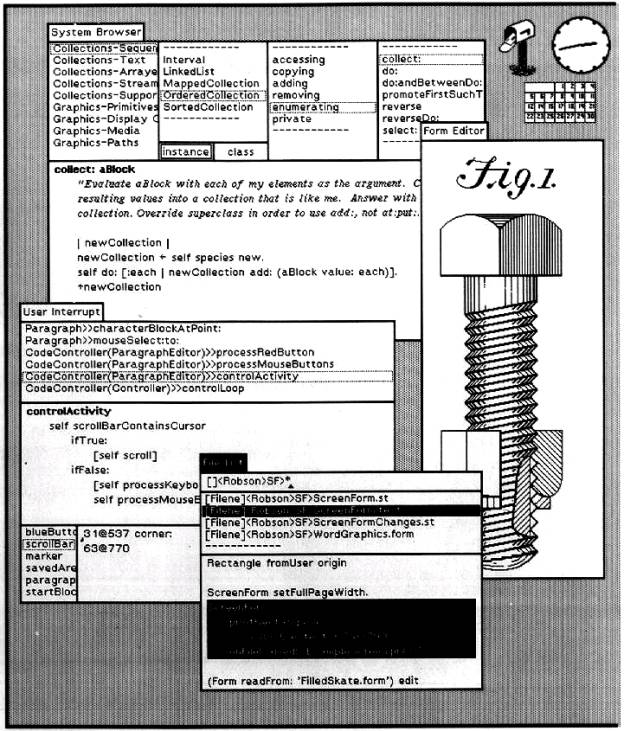
\includegraphics[width=0.5\textwidth]{images/smalltalk}
    %\vspace{-15pt}
    \caption{Smalltalk user interface.}
    \vspace{-20pt}  
  \label{fig:smalltalk}
\end{wrapfigure} 

Smalltalk programming environment was a successful achievement with relevant improvements on its successors. The system consisted of about 50 classes described in about 180 pages of source code~\citep{Kay1993}. This included all of the OS functions, files, printing and other Ethernet services, the window interface, editors, graphics and painting systems, as shown in Figure~\ref{fig:smalltalk}. 

In the Smalltalk programming language, the communication through messages has a strong resonant metaphor. To specify the behavior of an object, the programmer casts himself into the role of that object (to the extent of referring to the object as ``self'') and thinks of himself as carrying on a conversation with other objects. This is a strong metaphor, because role-playing and conversing are innate human facilities. 

In fact, SmallTalk features are, nowadays, a consistent reference for any programming system.
%%%%%%%%%%%%%%%%%%%%%%%%%%%%%%%%%%%%%%%%%%%%%%%%%%%%%%%%%%%%%%%%%%%%%%%%%%%%%%%%%%%%%%%%%%%%%%%%%%%%%%%%%
\subsection{Processing}
\label{subsec:processing}
Processing~\citep{Reas2006} is a programming language and environment designed to teach programming in a visual context. Processing has become popular among students, artists, designers, and architects, because it acts as a tool to get non-programmers started with programming through instant visual feedback.

The Processing programming language is built on top of Java, but it removes much of the verbosity of Java to make the syntax accessible to novices. The language provides simple access to external libraries, such as OpenGL, through single entry points, such as \texttt{setup} and \texttt{draw}. This allows novices to quickly prototype, learn fundamental concepts of programming, and, eventually, gain the basis to learn other programming languages.

The programming environment contains a simple text editor, a text console to present errors, and a run button. The run button compiles the Processing code and executes it. Despite in the default mode the result is presented in a 2D graphical window, the render can be configured to present the result in 3D or in other sophisticated methods using \textit{shaders} to recur directly to the graphic board.

Actually, with a few changes, the Processing code can be exported as an application for different platforms, such as Java, JavaScript, and Android. For example, to export a Processing program for JavaScript, it is only necessary to create a HTML page and include the Processing code as a script of this page. Then the Processing code will be automatically parsed and translated to JavaScript. To maintain the usual render capabilities of a Processing program it will use the HMTL5 canvas with WebGL.

The popularity of Processing is explained by the benefits of these features, besides of being a domain-specific language, however it has drawbacks that can discourage its use, such as the following:

\begin{itemize}
  \item \textit{Weak metaphor}. The Processing programming language, by contrast with the above systems, has none strong metaphors that allow the programmer to translate his experiences as a person into programming knowledge. 

  \item \textit{Poor decomposition}. Processing discourages the fundamental approach to solving a complex problem by breaking it into simpler problems, because drawing and input events are tied to single entry points. Thereby the behavior of submodules must be tangled across these global functions, making it difficult to achieve clean decomposition.

  \item \textit{Poor recomposition}. Processing discourages combining two programs. The programmer cannot just grab and use part of other programs, because variables must be renamed or manually encapsulated, and the \texttt{draw} and mouse functions must be woven together. Even worse, Processing has global modes which alter the meaning of the function arguments. For example, two Processing programs can specify its colors in different modes and each mode has its proper meaning of \texttt{fill} function arguments. Combining those programs will be almost impossible. 

  \item \textit{Weak readability}. The syntax of a Processing program represents a significant barrier for reading. For example, the function which draws an ellipse on screen is written as \texttt{ellipse(50,50,100,100)}. The reader must lookup or memorize the meaning of every single argument.

  \item \textit{Fragile environment}. The programming environment is fragile, because it does not attempt to solve any of the above issues related with the language and its implementation.
\end{itemize}

%%%%%%%%%%%%%%%%%%%%%%%%%%%%%%%%%%%%%%%%%%%%%%%%%%%%%%%%%%%%%%%%%%%%%%%%%%%%%%%%%%%%%%%%%%%%%%%%%%%%%%%%%
\subsection{Fluxus}
\label{subsec:fluxus}
Fluxus~\citep{griffiths2007fluxus}\footnote{\texttt{http://www.pawfal.org/fluxus/}} is a programming language and learning environment designed for rapid prototype using 3D graphics and sounds. This emphasis on rapid prototype and quick feedback makes Fluxus a tool for learning computer animation, graphics and programming. However, most users of Fluxus use it for \textit{livecoding}, which is the act of performing coding lively to an audience.

Fluxus is mainly written in C++ and it is statically linked to several shared libraries, specified at compile time. For instance, Fluxus uses \texttt{jack-audio}, \texttt{ode}, and \texttt{fftw} libraries to handle and synchronize the audio, \texttt{GLEW} to present graphics, and \texttt{racket3m} to embed the Racket run-time system into the application. In this way, Fluxus is an extension of Racket (a descendant of Scheme) with graphical commands.

Like Processing, Fluxus provides simple access to those libraries through single entry points, for instance \texttt{start-audio} connects an input audio to the application, \texttt{every-frame} registers a function called once per frame, and so on. However, as stated above, it is a barrier for decomposition since the behavior of submodules must be tangled across these global functions.

\begin{figure}[!htbp]
  \centering
  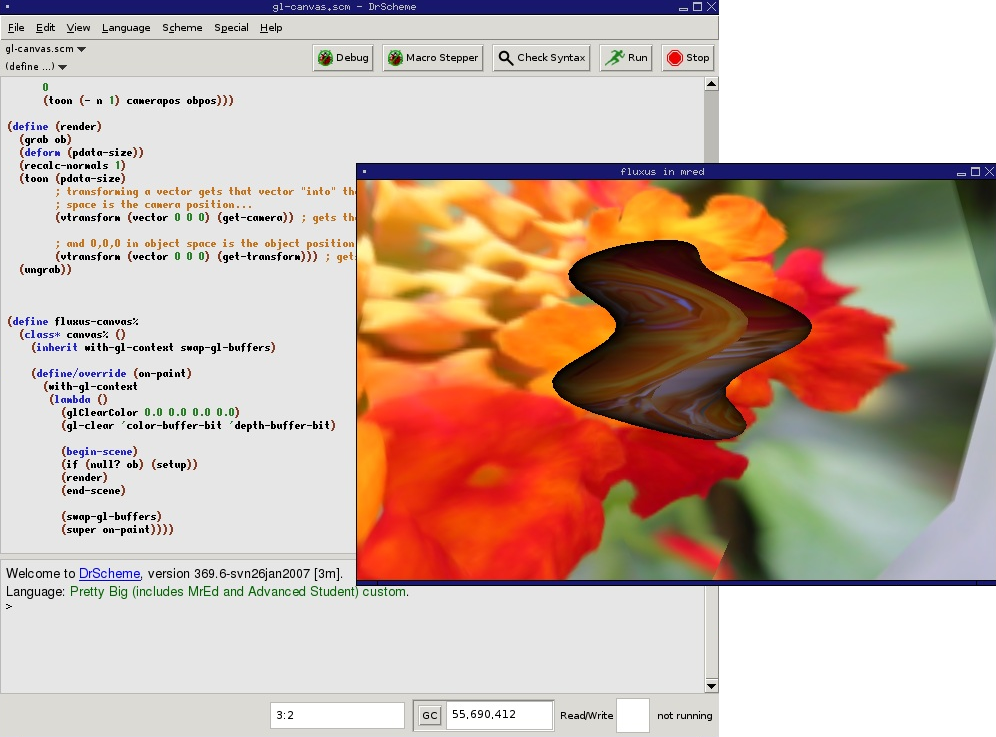
\includegraphics[width=.8\textwidth]{images/fluxus}
    \caption{Fluxus engine being used as DrRacket module}
  \label{fig:fluxus}
\end{figure} 

Fluxus has its own environment specifically tailored for \textit{livecoding}. It is composed by a OpenGL graphical window with a simple text editor. The programmer types his code in the editor and presses a shortcut key each time he wants to run the code. Fluxus evaluates the code through Racket run-time system and shows its result in the same graphical window that the code was written. This mechanism is valuable in an \textit{livecoding} environment, because the performer can be editing the code while the result of the previous computation is maintained in background. However, if the code has any error and the performer execute it, the previous computation disappears and the environment will not help to find it. This is a serious problem, specially for the Racket syntax.

Moreover, Fluxus shares with Processing similar drawbacks to those previously stated. However Fluxus can be used as a module of DrRacket (Figure~\ref{fig:fluxus})~\citep{findler2002drscheme} programming environment and, fortunately, in DrRacket the above problem and many others are solved.
%%%%%%%%%%%%%%%%%%%%%%%%%%%%%%%%%%%%%%%%%%%%%%%%%%%%%%%%%%%%%%%%%%%%%%%%%%%%%%%%%%%%%%%%%%%%%%%%%%%%%%%%%
\subsection{DrRacket}
\label{subsec:drracket}
DrRacket~\citep{findler2002drscheme} is a programming environment designed to support the Racket language. DrRacket is one of few programming environments which supports gradual learning in a more general language from the start. Consequently, it has been widely used in introductory programming courses in several universities around the world.

The usual scenario where DrRacket is used is to teach functional programming using Racket. To facilitate this process, DrRacket provides three tools. The first is a symbolic stepper. It models the execution of Racket programs as algebraic reductions, since Racket is implemented on top of lambda calculus. The second tool is a syntax checker. It annotates programs with font and color changes based on the syntactic structure of the program. It also permits students to explore the lexical structure of their programs graphically and to $\alpha$-rename identifiers. The third tool is a static debugger that infers which set of values an expression may produce and how values flow from place to place in the source text, and, upon demand, it explains the reason of errors by drawing value flow graphs over the program text.

Similar to Lisp environments, DrRacket provides a read-eval-print loop (\gls{repl}). This is a command prompt intended to quickly evaluate expressions and print their results. Especially in a learning environment, this feature makes an important connection between program execution and algebraic expression evaluation. However, the Lisp-style syntax obscures the effect of this feature. To overcome this limitation, DrRacket provides a \texttt{pretty-printer}. A module capable of printing algebraic expressions in a meaningful way, as well as other graphics elements supported by the text editor, such as images, snips, XML boxes, and so on.

More recently, DrRacket has included picture boxes for \gls{wysiwyg} layout of slide content that is otherwise created programmatically~\citep{findler2004slideshow}. This kind of presentation extensibility is in addition to recognizing standard Racket hygienic macros. There are several problems with this approach. First, there is no documented protocol for creating new kinds of boxes. Second, any program that uses boxes is stored as ascii-encoded binary and is difficult to edit outside of DrRacket. Last, the semantics of the boxes is driven off of the display itself, rather than the persistent store; therefore, in order to compile, interpret, or edit the program, a box-aware editor is required.

From the perspective of professional programmers DrRacket can be a potential target. It is useful for developing complex applications, including DrRacket itself. Moreover it is extensible by the same \gls{api} which the above tools implement. Through this \gls{api} it is also possible to extend the \gls{repl}, as in Pict3D\footnote{\texttt{https://github.com/ntoronto/pict3d}} (a 3D engine that integrates new graphical elements in the DrRacket environment). On the other hand, for supporting extensions, DrRacket's architecture has become increasingly complex. For instance, to make a simple change in an editor's element the programmer should be able to understand several modules, unrelated with the problem itself. This extra complexity is a negative impact when DrRacket is chosen as basis for new development tools.

Despite of the identified advantages, DrRacket has some barriers that may discourage the learner. For example, the Racket programming language is simple to teach, but its heavy syntax of s-expressions hinders the learner to read the program. Consequently, the learner can spend a huge mental effort to understand insignificant details of the language.
%%%%%%%%%%%%%%%%%%%%%%%%%%%%%%%%%%%%%%%%%%%%%%%%%%%%%%%%%%%%%%%%%%%%%%%%%%%%%%%%%%%%%%%%%%%%%%%%%%%%%%%%%
\subsection{PythonTutor}
\label{subsec:pythontutor}
PythonTutor~\citep{GuoSIGCSE2013} is a web-based program visualization tool, designed to explain how a piece of Python code executes. It has become popular among students from introductory Computer Science courses. Using this tool, teachers and students can write Python programs directly in the web browser and navigate step by step throughout its execution, seeing the run-time state of data structures.

PyhtonTutor has two main modules: the \textit{backend} which implements the tool core functionality, and the \textit{frontend} which presents the visualization of program's data structures. The \textit{backend} executes the input program under supervision of the standard Python debugger module (\texttt{bdb}) which stops execution after every executed line and records the program's run-time state. After execution terminates, the \textit{backend} encodes the program state in JSON format, serializing Python data types into native JSON types with extra \textit{metadata} tags and sends it to the \textit{frontend}. The frontend renders the objects using standard web technologies: HTML, CSS, and JavaScript. In this way, users can use the tool without installing any extensions or plugins.

A major concern in PythonTutor is security, because the PythonTutor's \textit{backend} executes untrusted Python code from the web. To prevent the execution of dangerous constructs such as {\tt eval}, {\tt exec} and {\tt file I/O}, PythonTutor implements sandboxing. Basically, it denies the use of most module imports, by parsing the user's code importing, a strict approach, but effective in this case.

The PythonTutor tool allows the programmer to follow the program execution over time, but he only sees a single point in time at any instant. There is no visual context at all. The entire program flow is represented by disconnected points in time. For example, the programmer who wants to understand a conditional algorithm, using this tool will not see the pattern of this algorithm neither understand it at a higher level.
%%%%%%%%%%%%%%%%%%%%%%%%%%%%%%%%%%%%%%%%%%%%%%%%%%%%%%%%%%%%%%%%%%%%%%%%%%%%%%%%%%%%%%%%%%%%%%%%%%%%%%%%%
\subsection{YinYang}
\label{subsec:yinyang}
YinYang~\citep{mcdirmid2013usable} is a prototype of a programming language and environment whose main feature is the live execution feedback. That means it combines editing and debugging, where updated debug results are conveniently visible while editing. YingYang addresses the above issue in two ways. First, just like the previous system, it allows programmers to see single points of execution directly within the code editor (probe; precede expressions with \texttt{@} operator). Second, it has a pane aside the editor which traces execution with entries that are navigable (trace; print-like statements). Basically, the trace is an enhanced display function which, combined with ``probes'', allows the state of previous executions to be restored. So, programmers can take in the entire program flow at a glance and navigate trough it using probes.

YingYang uses an incremental framework as basis of its programming model. This framework decomposes the program execution into a tree of nodes that can be re-executed independently on a code or input change. However, this decomposition cannot be performed transparently. It requires programmers to specify how the program will be decomposed. To perform this task one must deeply understand the granularity and modularity characteristics of the computations being performed by the program. Otherwise changes can sometimes have a huge impact on program re-execution time ($\sim$50ms). Consequently, live programming would actually reduce programmer productivity as programmers wait for slow feedback.

Although YinYang provides usable features for a learning environment, such as the live execution feedback, it does not have a suitable language for beginners. The language is merely experimental and to navigate through the program execution, programmers must include probes in the code. At the end of experimentation, the code is full of useless expressions.

%%%%%%%%%%%%%%%%%%%%%%%%%%%%%%%%%%%%%%%%%%%%%%%%%%%%%%%%%%%%%%%%%%%%%%%%%%%%%%%%%%%%%%%%%%%%%%%%%%%%%%%%%
\section{Empowering Systems}
\label{sec:es}
In this category of systems the most important aspect is to allow people to build programs tailored to their own needs. In this section, I describe how systems from two distinct areas are tailored to achieve their user's needs. 

First, I consider Architecture, where new programming languages and environments are being proposed to support the increasing use of \gls{gd}~\citep{mccormack2004generative}. \gls{gd} is a design method that uses algorithms to generate architectural models. Usually these models are rendered using a \gls{cad} tool. 

Second, I consider Mathematics, where advanced technologies are used to approximate as much as possible the mathematical models to the ones that we can see and understand.

%%%%%%%%%%%%%%%%%%%%%%%%%%%%%%%%%%%%%%%%%%%%%%%%%%%%%%%%%%%%%%%%%%%%%%%%%%%%%%%%%%%%%%%%%%%%%%%%%%%%%%%%%
\subsection{DesignScript}
\label{subsec:designscript}
DesignScript~\citep{aish2012designscript} is a programming language and environment designed to support \gls{gd} with textual methods. It is mainly used by architects and designers to generate geometric models using a script. When the script is executed it generates new models in a \gls{cad} tool. DesignScript is a AutoDesk\footnote{\texttt{http://www.autodesk.com/products}} product initially proposed to be used within AutoCAD (as shown in Figure~\ref{fig:ds}), nowadays it provides the same functionality on top of Revit, another AutoDesk product used for \gls{bim}. In short, a \gls{bim} model is similar to a \gls{cad} model but it covers more than just geometry. It also covers spatial relationships, properties of building components, such as manufacturers' details.

\begin{figure}[!htbp]
%\vspace{-5pt}
  \centering
  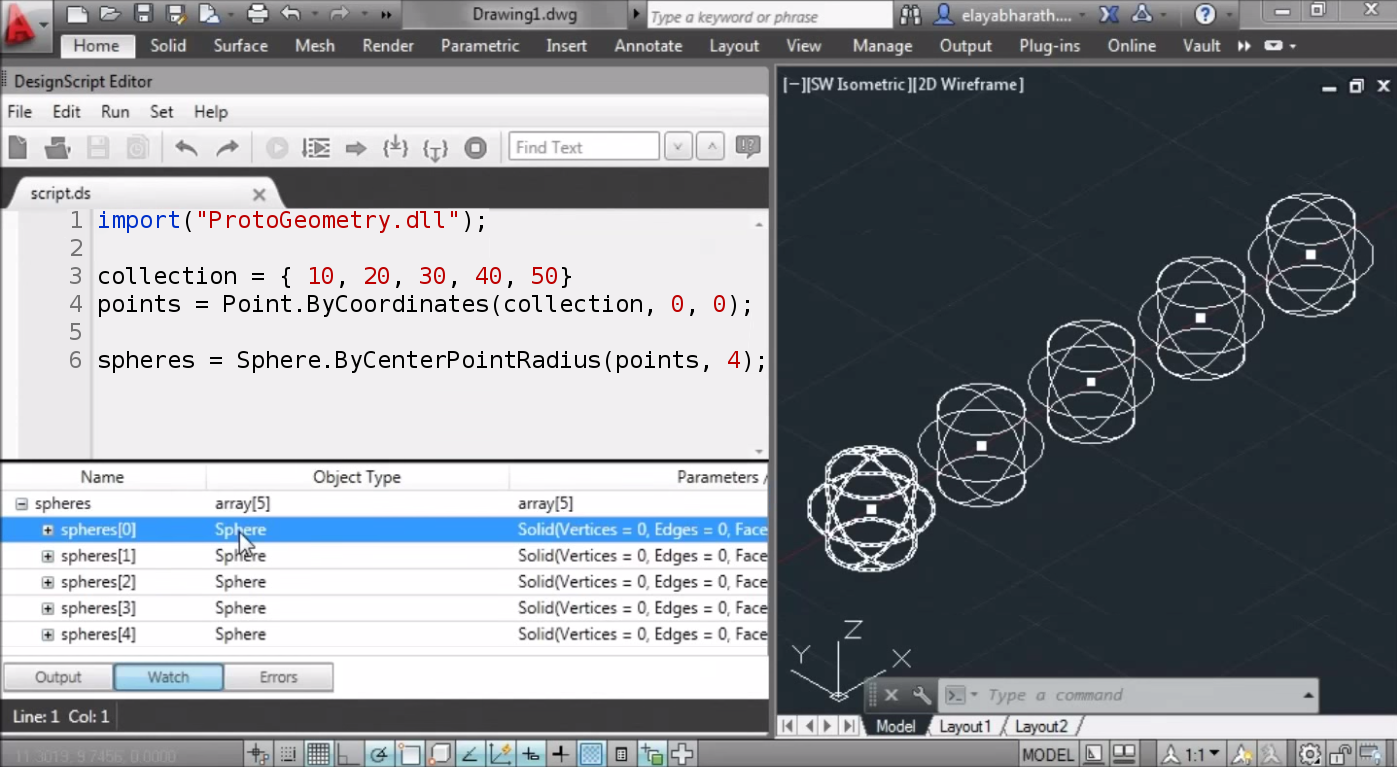
\includegraphics[width=1.0\textwidth]{images/designScriptIDE}
 % \vspace{-15pt}
    \caption{Typical DesignScript programming environment} 
  %  \vspace{-10pt} 
  \label{fig:ds}
\end{figure} 

The programming language is presented as an associative language. The variables are abstract types that can represent numeric values or geometric entities. These variables are maintained in a graph of dependencies. When a change in a variable occurs it forces the re-evaluation of the graph, as shown in Figure~\ref{fig:designscript}, consequently variables has always updated values. This feature is useful, specially in a modeling environment, because it provides continuous feedback to the designer as the model is being modified.

\begin{wrapfigure}{r}{0.45\textwidth}
  %\vspace{-5pt}
  \begin{center}
    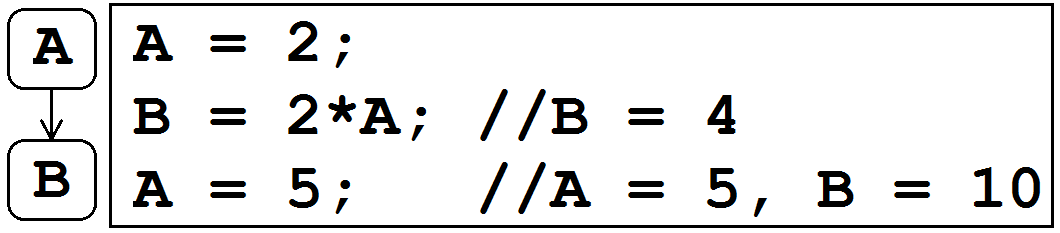
\includegraphics[width=0.45\textwidth]{images/designscript}
  \end{center}
  %\vspace{-20pt}
 \caption{Associative interpretation}  
  %\vspace{-20pt}
    \label{fig:designscript}
\end{wrapfigure}

The DesignScript's programming environment provides a text editor, an interpreter, and a simple debugger. The language interpreter is invoked each time that the designer clicks on the run button. Then all the script is interpreted and its result produces geometric entities rendered in the \gls{cad}. The continuous feedback feature works only in debug mode, because in this mode the script is interpreted line by line. Thus, each update to a variable will change its dependencies and will recompute the model. However, in debug mode the code cannot be edited, so this feature is worthless during code editing.

In the DesignScript's debug mode, users can inspect the variable values by adding \textit{watchers} to them. A watched variable is showed in a special tab, as shown in Figure~\ref{fig:designscript}. In case the variable represents a geometric model, the respective model will be highlighted in the \gls{cad} when the variable is selected. It creates a certain \textit{traceability} between models in the \gls{cad} and code in the editor. In this way the user is able to correlate which model a variable corresponds to. However the inverse, starting form the model and finding the correspondent variable, is unsupported.

DesignScript also supports a typical mechanism of \textit{live} programming environments: the sliders. The sliders are widgets which facilitate giving new values to the program input. This way, designers can create new models reacting to these changes. However, in the DesignScript's sliders the changes are reflected in the models only when the designer leaves the slider. Until then, the designer should imagine how the model would be with the new value, which is completely against the purpose of sliders.

Moreover the DesignScript language, despite of being presented as pedagogic, has some drawbacks. It does not carry any strong metaphor which helps beginners start with the language. Additionally the associative paradigm represents a barrier for sharing code: it discourages the recomposition of modules, because new modules can change the previous one. The environment provides poor mechanisms that help people to find bugs in the code, and finally,  DesignScript is confined to produce geometry in a single \gls{cad} tool.
%%%%%%%%%%%%%%%%%%%%%%%%%%%%%%%%%%%%%%%%%%%%%%%%%%%%%%%%%%%%%%%%%%%%%%%%%%%%%%%%%%%%%%%%%%%%%%%%%%%%%%%%%
\subsection{Monkey} 
\label{subsec:monkey}
Monkey\footnote{\texttt{http://wiki.mcneel.com/developer/monkeyforrhino4}} is a programming environment designed to support \gls{gd}. Like DesignScript, Monkey is used to edit, debug and interpreter scripts. However, Monkey uses RhinoScript as its programming language and Rhinoceros3D\footnote{\label{fnote:rhin}\texttt{https://www.rhino3d.com}} (or Rhino for short), a lighter \gls{cad} than AutoCAD, to generate the geometric models.

Monkey is implemented as a \texttt{.NET} plugin for Rhino4 and provides a programming environment to write and debug scripts. The RhinoScript is based on Microsoft's VBScript language (a descendant of BASIC), and like VBScript it is a weakly typed language. One of the major drawback with this language is the fact that users must beware with the data passed in their functions at all time, because RhinoScript can accidentally casts variables into inappropriate types. Therefore, it creates errors difficult to find, specially for people which are learning to program.

Monkey is based on general-purpose programming environments. It provides typical features of those environments, namely syntax highlighting, auto-completion, and error highlighting. The organization of code into trees is also similar. However, the programming environment and language, does not provide any well designed feature which helps beginners to start with programming. The provided features are based on general-purpose systems, instead of being tailored for \gls{gd}.
%%%%%%%%%%%%%%%%%%%%%%%%%%%%%%%%%%%%%%%%%%%%%%%%%%%%%%%%%%%%%%%%%%%%%%%%%%%%%%%%%%%%%%%%%%%%%%%%%%%%%%%%%
\subsection{Rosetta}
\label{subsec:rosetta}
Rosetta~\citep{lopes2011portable} is a programming environment designed to support \gls{gd} that is based on DrRacket~\citep{findler2002drscheme}. Like Monkey, Rosetta provides its own environment detached from the \gls{cad}. Rosetta is a step forward from the previous systems, because it solves the portability problem among \gls{cad} tools. In Rosetta a \gls{gd} program can be written in various programming languages (frontends) and the geometric models can be rendered by various \glspl{cad} (backends). As a result, designers are free to write their programs in their preferred frontend which, upon execution, will generate the same geometry for the various backends. In Figure~\ref{fig:rosetta}, a program is written in Racket and its execution produces geometry for AutoCAD.

\begin{figure}[!htbp]
%\vspace{-5pt}
  \centering
  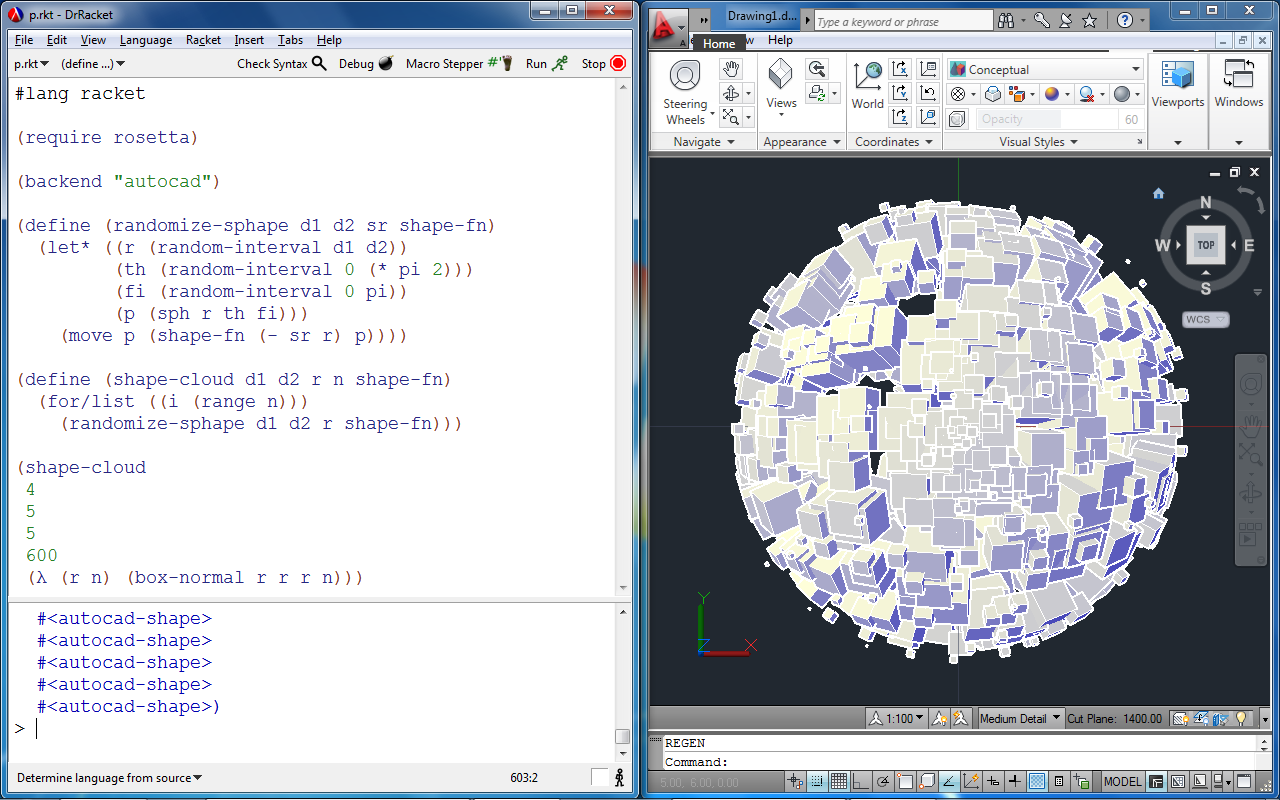
\includegraphics[width=1.0\textwidth]{images/rosetta1}
  %\vspace{-20pt}
    \caption{Rosetta programming environment.}  
  \label{fig:rosetta}
  %\vspace{-10pt}
\end{figure} 

Rosetta has been used to teach programming in architecture courses. Tailored to this end, Rosetta uses DrRacketas its own programming environment. The DrRacket environment serves a number of functions, but the most important is that the student can start immediately to learn programming. For instance, the environment is set up with just three lines of code. As shown in Figure~\ref{fig:rosetta}, the \texttt{\#lang} specifies the frontend language, the \texttt{require} imports Rosetta's primitives and finally the \texttt{backend} names a possible backend.

The Racket language is also an advantage of Rosetta's environment, because it encourages the use of the mathematical paradigm for writing algorithms. In this way, students that learn simple programming techniques, such as recursion, are able to create robust models. Additionally, as the students progress, new programming languages are also available to learn, such as JavaScript, Python, Processing, and so on.

The Rosetta's environment provides some interesting tools for \gls{gd}, such as a programming flow tracer, similar to the DesignScript's watcher. It highlights models in the \gls{cad} upon selection of expressions, it also supports the inverse, selecting the model in the \gls{cad} and shows the expression in the code editor. Another interactive tool is the slider, an attempt to provide immediate feedback to the designers. It uses the DrRacket slider, associating the slider callback to the function that generates the entire model, so each time the slider change a new model will be generated. However, this process must be performed manually.

Undoubtedly Rosetta's environment goes further than the textual environments for \gls{gd} presented in this report. However it presents some drawbacks which may discourage the learning in general. Beginning with the usual programming language: Racket. The syntax of a Racket program represents a significant barrier for reading. For instance the function which draws a circle in Rosetta is written as \texttt{(circle (xy 0 0) 1)}. The reader must lookup or memorize every argument. Using the Rosetta's documentation the reader will spend even more time, because it is in a book mixed with architecture topics.
%%%%%%%%%%%%%%%%%%%%%%%%%%%%%%%%%%%%%%%%%%%%%%%%%%%%%%%%%%%%%%%%%%%%%%%%%%%%%%%%%%%%%%%%%%%%%%%%%%%%%%%%%
\subsection{Grasshopper}
\label{subsec:grasshopper}
Grasshopper\footnote{\texttt{http://www.grasshopper3d.com/}} is a programming language and environment designed to support \gls{gd} using a visual language. Grasshopper provides an alternative way to programming. By definition, it is a bi-dimensional representation consisting of iconic components that can be interactively manipulated by the user according to some spatial grammar~\citep{myers1990taxonomies}. For example, the boxes in Figure~\ref{fig:grass} are components which receive the input (left ports) perform some operations and return the output (right port). The components are linked to other components establishing a \textit{dataflow} paradigm where the input of a component is the output of another.

\begin{figure}[!htbp]
%\vspace{-5pt}
  \centering
  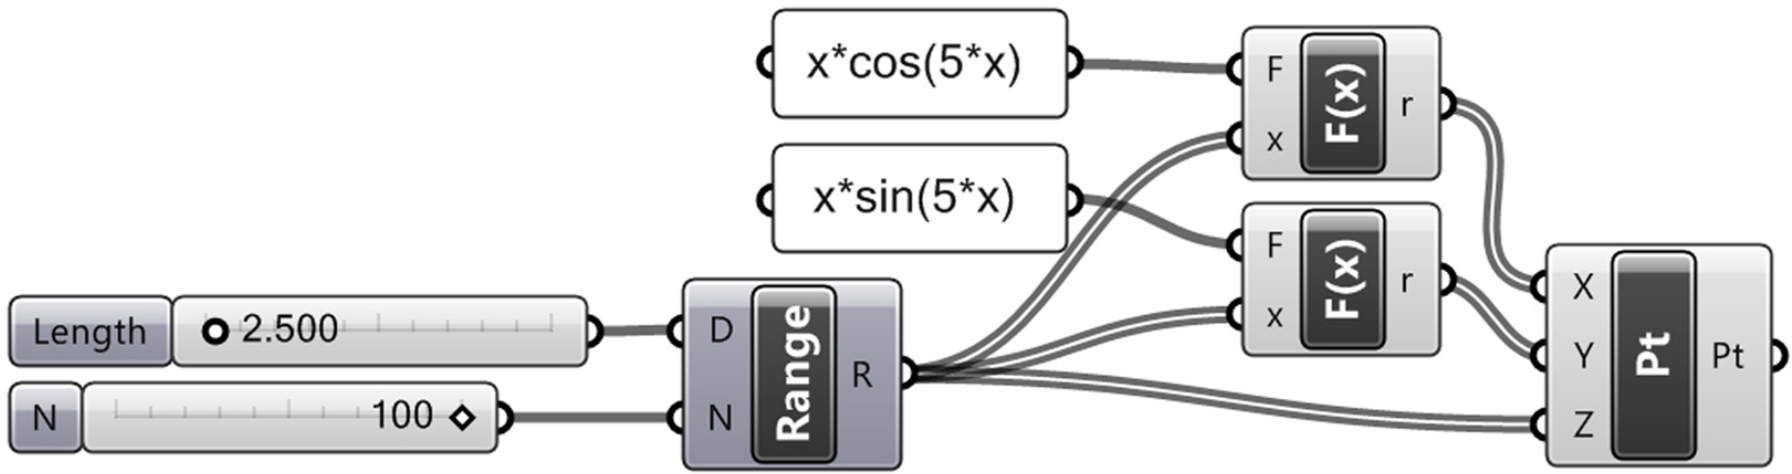
\includegraphics[width=0.8\textwidth]{images/grasshopper}
  %\vspace{-5pt}
    \caption{A program in Grasshopper that computes the 3D coordinates of a conical spiral. Each time the left sliders are dragged a new coordinate is calculated.}
  \label{fig:grass}
  %\vspace{-10pt}
\end{figure}

Like Monkey, Grasshopper is implemented as a \textit{plugin} for Rhino$^{\ref{fnote:rhin}}$. However Grasshopper tailors the Rhino's environment with specific \gls{gd} tools. These tools are state of the art, because they implement important principles for design models, such as the following:

\begin{itemize}
 \item \textit{Get immediate feedback}. As the user interacts with the components, by adding and connecting them, the result reflects immediately in the \gls{cad} model. It facilitates the design conception, because the user's intentions are immediately visible. 
 \item \textit{Facilitate program input}. To facilitate the process of design exploration, Grasshopper provides sliders which are connected at the component input. Dragging the slider causes a change propagation through components. The components are re-executed with the new slider value. Combined with the above feature new models are generated immediately.
 \item \textit{Correlate the program with the generated elements}. Like DesignScript's watcher, by selecting a component its geometry is highlighted in the \gls{cad}. It allows designers to better understand a program by figuring out the roles of each component.
 \item \textit{Show comparisons between models}. Grasshopper provides a special component that, when connected at the output of another component, replicates the geometry. This mechanism is useful for design exploration, because it maintains in the \gls{cad}'s background an old replica of the changed geometry. It adds a context at each change, so the designer can compare the result of his change in the new geometry based on the old one.
\end{itemize}

Mainly, the Grasshopper interactivity depends on the immediate feedback tool. However, this tool will never scale for arbitrarily complex programs, because the \gls{cad}'s render is not designed to process the huge amount of information generated by \gls{gd} methods. Other systems, such as DesignScript and Rosetta, improve this problem by sidestepping most of the functionality of traditional \gls{cad} tools and focusing only on the generation and visualization of geometric models. These systems provide a backend based on OpenGL that is independent of a full-fledged \gls{cad} application, but, in Grasshopper, there is no such backend.

Moreover, the traceability among components is just in one direction. From the designer perspective, it would be more useful start form the geometry and find which component implements it, but it is unsupported. However, despite the usefulness of model comparison in design exploration, this feature is also unsupported.
%%%%%%%%%%%%%%%%%%%%%%%%%%%%%%%%%%%%%%%%%%%%%%%%%%%%%%%%%%%%%%%%%%%%%%%%%%%%%%%%%%%%%%%%%%%%%%%%%%%%%%%%%
\subsection{Dynamo}
\label{subsed:dynamo}
Dynamo\footnote{\texttt{http://dynamobim.com/}} is a programming language and environment designed to support \gls{gd}. Like Grasshopper, Dynamo provides an alternative way to programming. However Dynamo, like DesignScript, is implemented on top of Revit, an Autodesk product for \gls{bim}.

\begin{wrapfigure}{r}{0.5\textwidth}
  %\vspace{-30pt}
  \begin{center}
    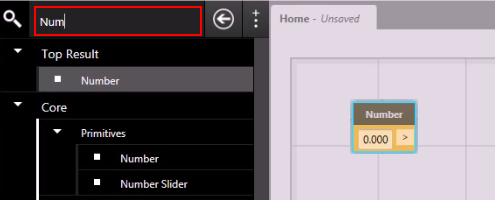
\includegraphics[width=0.5\textwidth]{images/dynam-tab}
  \end{center}
  %\vspace{-18pt}
 \caption{Dynamo search tab. Searching for a component, highlighted in red.}  
  %\vspace{-20pt}
    \label{fig:dynam}
\end{wrapfigure}

Dynamo provides a set of tools similar to Grasshopper, particularly a searching table, as shown in Figure~\ref{fig:dynam}, which provides quick access to the primitives of the language, such as the components and widgets. This feature encourages designers to explore the available components and try new components.

In general, Dynamo and Grasshopper are programming environments and visual languages popular among novices in programming. The smooth learning curve and perhaps the style of the \gls{ui} elements are attractive for beginners. However as the visual programs become large and complex it requires more time to understand, maintain, and adapt to new requirements, than the textual programs as showed in~\citep{leitao2011programming}. Despite spending more time and effort to learn a textual programming language, the learners have their time quickly recovered once the complexity of the design task becomes sufficiently large.
%%%%%%%%%%%%%%%%%%%%%%%%%%%%%%%%%%%%%%%%%%%%%%%%%%%%%%%%%%%%%%%%%%%%%%%%%%%%%%%%%%%%%%%%%%%%%%%%%%%%%%%%%
\subsection{Mathematica}
\label{subsec:mathematica}
Mathematica~\citep{wolfram1991mathematica} is a language and environment built to support scientific calculation. It is widely used in the scientific community, specially by students, because it represents programs using a short and clear artificial language. This language supports not just linear textual input, but also two-dimensional input, like traditional mathematical notation.

\begin{figure}[!htbp]
%\vspace{-5pt}
  \centering
  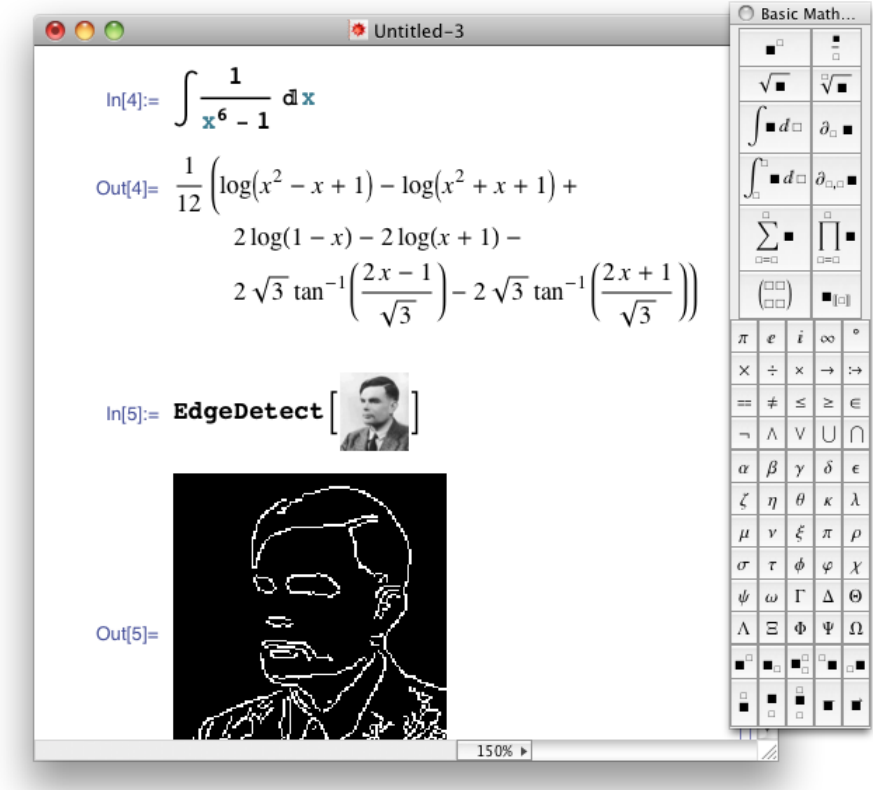
\includegraphics[width=.7\textwidth]{images/mathematica}
  %\vspace{-20pt}
    \caption{Mathematica notebook}  
  \label{fig:math}
  %\vspace{-10pt}
\end{figure} 

The core concepts of Mathematica are based in the paradigm initiated by Turing's work~\citep{wolfram2003wolfram}. In this paradigm mathematical processes are systematized as computations. For example, in a typical interaction, the user types a mathematical expression in the Mathematica environment (i.e. notebook), then this expression is evaluated, as shown in Figure~\ref{fig:math}.  

A relevant aspect of Mathematica's notebook is the immediacy that users get a response. Unlike a typical program that must be executed explicitly to get a feedback of an action, in this notebook expressions are evaluated as soon as they are typed. It works like a read-eval-print loop, however it has enhanced mechanisms to present data meaningfully.

The Mathematica features are well designed to present data in a human readable form. It would be useful for an external programming languages, if it could take advantage of these features. Unfortunately, Mathematica is closed for this end.
%%%%%%%%%%%%%%%%%%%%%%%%%%%%%%%%%%%%%%%%%%%%%%%%%%%%%%%%%%%%%%%%%%%%%%%%%%%%%%%%%%%%%%%%%%%%%%%%%%%%%%%%%
\subsection{IPython}
\label{subsec:ipython}

IPython~\citep{PER-GRA:2007} is a programming environment built to support scientific calculation. Unlike Mathematica~\citep{wolfram1991mathematica},  IPython is an open platform for extensions, it allows external programming languages (frontends) to use its features which includes an interactive shell, and a browser-based notebook with support for code, text, mathematical expressions, plots, and other rich media. 

Like Mathematica, IPython has a notebook where users can try out expressions and immediately see its result, as shown in Figure~\ref{fig:ipython}, however this notebook is in a web format. IPython's architecture is a typical client-server, where the frontend is the client (i.e. the notebook), and the server is a language kernel (i.e. the programming language which users interact with). The communication between client and server, is through a strict protocol that the language kernel must implement. 

\begin{figure}[!htbp]
  \centering
    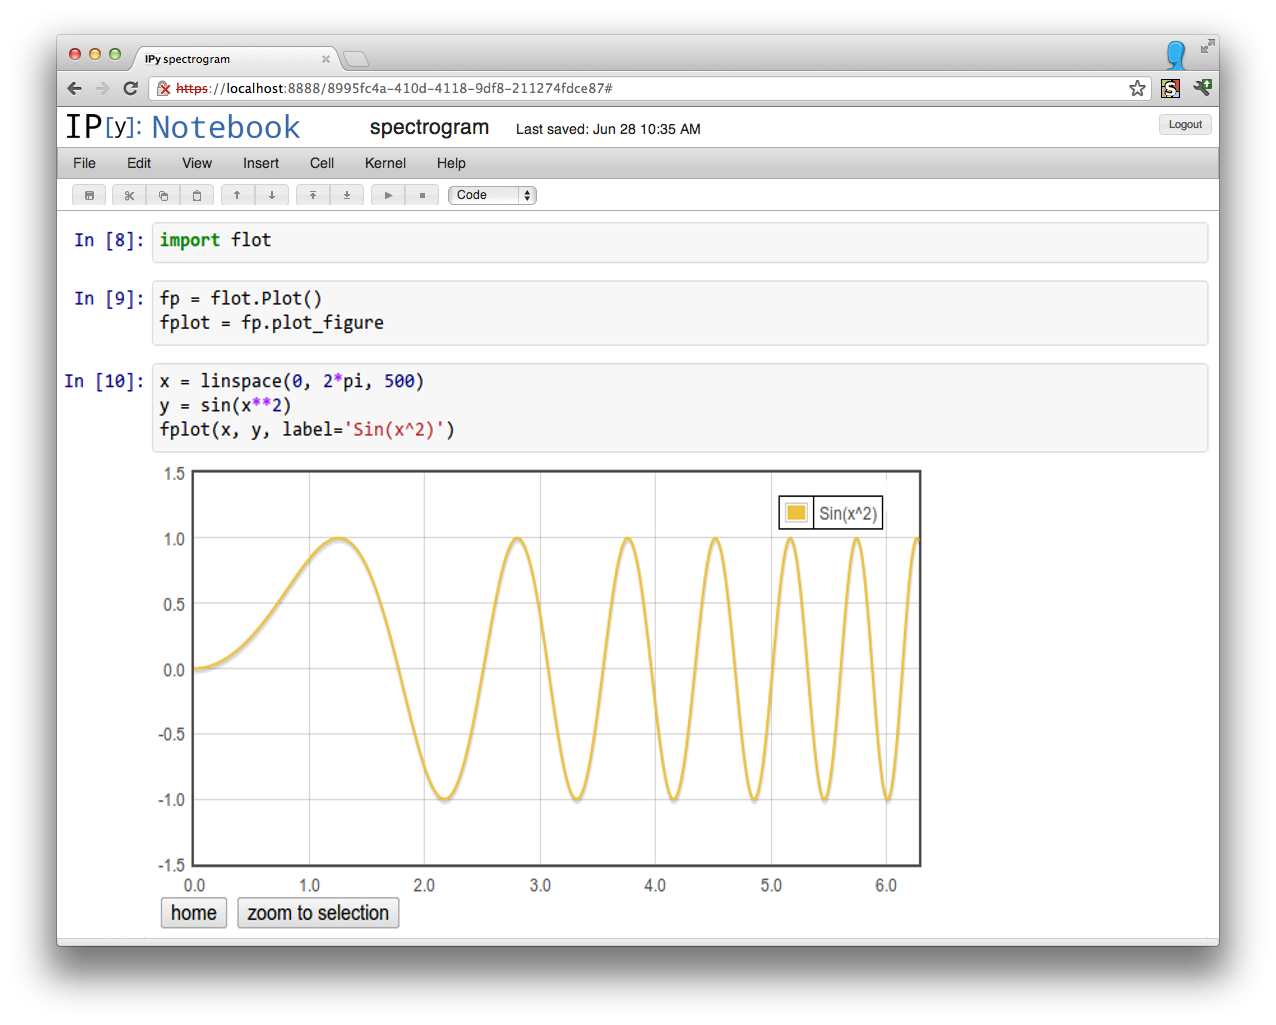
\includegraphics[width=0.7\textwidth]{images/ipython}
 \caption{IPython browser-based notebook}
    \label{fig:ipython}
\end{figure}

IPython provides a base layer for new programming environments, by exposing the major components of its architecture, consequently its features are available from other systems. For example, IJulia uses IPython interface with Julia language. 
%%%%%%%%%%%%%%%%%%%%%%%%%%%%%%%%%%%%%%%%%%%%%%%%%%%%%%%%%%%%%%%%%%%%%%%%%%%%%%%%%%%%%%%%%%%%%%%%%%%%%%%%%
\subsection{MathCAD}
\label{subsec:mathcad}
MathCAD\footnote{\texttt{http://www.ptc.com/product/mathcad}} is a programming environment and language built to support scientific calculation. Like Mathematica, MathCAD aims to present information into a human readable form. However, it generates live calculations with graphical plots, text and images into a single document. This document is the program environment as well as the final product.

The mathematical expressions defined in the MathCAD document act as an associative language. So, when an expression is changed its value is propagated through the document. This mechanism is the base of the interactiveness. However, it represents a barrier for program recomposition, because new expressions can change the previous ones. That means that variables has a global scope, the MathCAD document, if in somewhere a variable is changed it will be changed in every occurrence in the document.   
%%%%%%%%%%%%%%%%%%%%%%%%%%%%%%%%%%%%%%%%%%%%%%%%%%%%%%%%%%%%%%%%%%%%%%%%%%%%%%%%%%%%%%%%%%%%%%%%%%%%%%%%%		     
\section{Summary}

Table~\ref{tab:sum} shows the presented systems based on their major design influences. The table is also intended to address the following questions:

\begin{table}[h]
%\vspace{0pt}
\centering
%\ra{1.0}
\resizebox{\textwidth}{!}{%
\begin{tabular}{@{}clllc@{}}
\toprule
\multicolumn{1}{l}{{\bf Type$^{(1)}$}} & {\bf System} & {\bf Main feature$^{(2)}$} & {\bf \begin{tabular}[c]{@{}l@{}}Support to understand \\ programs$^{(3)}$\end{tabular}} & {\bf Representation of code$^{(4)}$} \\ \midrule
\multirow{6}{*}{GS} & Eclipse & \multirow{4}{*}{\begin{tabular}[c]{@{}l@{}}support software \\ development life cycle\end{tabular}} & \multirow{4}{*}{debugger} & \multirow{16}{*}{text} \\
 & NetBeans &  &  &  \\
 & IntelliJ &  &  &  \\
 & MVS &  &  &  \\ \cmidrule(lr){2-4}
 & Xcode & \multirow{2}{*}{observable programming} & \multirow{2}{*}{live execution feedback} &  \\
 & LightTable &  &  &  \\ \cmidrule(r){1-4}
\multirow{7}{*}{TS} & LOGO & \multirow{2}{*}{understandable language} & \multirow{2}{*}{physical interpretation} &  \\
 & SmallTalk &  &  &  \\ \cmidrule(lr){2-4}
 & Processing & \multirow{2}{*}{visual context} & \multirow{2}{*}{instant visualization} &  \\
 & Fluxus &  &  &  \\ \cmidrule(lr){2-4}
 & DrRacket & gradual learning & debugger; stepper &  \\ \cmidrule(lr){2-4}
 & PythonTutor & \multirow{2}{*}{show program flow} & \multirow{2}{*}{\begin{tabular}[c]{@{}l@{}}navigate through the \\ program execution\end{tabular}} &  \\
 & YinYang &  &  &  \\ \cmidrule(r){1-4}
\multirow{8}{*}{ES} & DesignScript & \multirow{3}{*}{\begin{tabular}[c]{@{}l@{}}support generative design \\ methods\end{tabular}} & \multirow{3}{*}{debugger} &  \\
 & Monkey &  &  &  \\
 & Rosetta &  &  &  \\ \cmidrule(l){2-5} 
 & Grasshopper & \multirow{2}{*}{\begin{tabular}[c]{@{}l@{}}alternative way to \\ expressing programs\end{tabular}} & \multirow{2}{*}{dataflow paradigm} & \multicolumn{1}{l}{\multirow{2}{*}{graphical components}} \\
 & Dynamo &  &  & \multicolumn{1}{l}{} \\ \cmidrule(l){2-5} 
 & Mathematica & \multirow{3}{*}{\begin{tabular}[c]{@{}l@{}}support scientific \\ calculation\end{tabular}} & \multirow{3}{*}{present data meaningfully} & \multicolumn{1}{l}{\multirow{3}{*}{mathematical forms}} \\
 & IPython &  &  & \multicolumn{1}{l}{} \\
 & MathCAD &  &  & \multicolumn{1}{l}{} \\ \bottomrule
\end{tabular}
}
%\vspace{1pt}
\caption{System attributes}
%\vspace{-20pt}
\label{tab:sum}
\end{table}

(1) \textit{What is the purpose of the system?} We categorized three main purposes for a system. \gls{gs} designed for building complex software for the industry; \gls{ts} designed to help people learn how to program; \gls{es} designed to help people build things that are tailored to their own needs.

(2) \textit{How does the system support its purpose?} We identified the following strategies: (i) support software development life cycle, (ii) turn programming in something more observable, (iii) create an understandable language, (iv) combine textual programming with a visual context, (v) support gradual learning in a single environment, (vi) show the program flow, (vii) support generative design methods, (viii) find alternative ways for to express programs, and (ix) support scientific calculation.

(3) \textit{Does the programming environment provide additional support to enable users to better understand the behavior of their programs?} Environments in our study used several techniques to help users understand the behavior of their programs. These included (i) a debugger which helps to find bugs in the program, (ii) an enhanced debugger which provides live execution feedback, (iii) languages with strong metaphor allowing physical interpretation, (iv) instant visualization of models, (v) navigation through the program's execution (vi) assembling components in a dataflow paradigm and (vii) present data adequately.

(4) \textit{How does code look in the programming environment or language?} The systems in our study represent programs using text, users can type, graphical components, users can manipulate, and mathematical forms users can fill in.

\section{Conclusion}

In the surveyed systems, the common representation of code is textual. This representation is typically static and, to be understood, requires the reader to know the vocabulary of the programming language. For a novice it is simply a barrier to learning. On the other hand, the representation of programs as graphical components or mathematical forms lowers this barrier, because for simple programs it is easier to read, but it becomes incomprehensible as the program grows.
%TEX root = ../dissertation.tex

\iffalse \bibliography{bibliography/dissertation} \fi

\chapter{Designing a Programming Environment for Generative Design}
\label{chapter:pegd}

\section{Design Principles} 

Programming is hard to learn. Unfortunately, as shown in the previous section, few programming languages or environments are designed to introduce the basics of good software engineering practice. Specially in Architecture, the environments used to support \gls{gd} either they are old or obsolete, or they enforce particular programming methods that are inadequate, or they are not pedagogic, meaning that they are not designed for the particular programming skills of the \gls{gd} community.

The literature is vast, but it is clearly divided in two perspectives: software engineering perspective, or psychological/educational perspective. That means either systems designed for expert programmers~\citep{carlson2005eclipse,intellij2001intellij,lighttable,boudreau2002netbeans,guckenheimer2006software}, or systems designed for novices~\citep{papert1980mindstorms,goldberg1983smalltalk,GuoSIGCSE2013,Reas2006}. The problem is that while programming systems designed for expert programmers are constantly updated, systems designed for novices are usually obsolete or in disuse. It negatively affects other communities that are not focused on develop software for industry, but for their own purpose which includes mainly novice users.

For example the \gls{gd} community is focused on build software to support Architecture methods, however designers are in desperate need of a programming system that correspond their needs. These needs are from different natures for instance: give support to the increasing adoption of \gls{gd} methods, deal with the increasingly complexity of current \gls{gd} programs, support tools that allows programs to be tested quicker, among others.

In the next section I propose...

\section{Program Documentation}

Program documentation is a software requirement of the utmost importance because it is a key factor for understanding programs. Even the best program, the most perfectly suitable for the job, will be essentially useless if the people who need to use it do not know what it is; cannot understand it well enough to use, build, or modify it; or (worst of all) misunderstand it and apply it incorrectly. And all of the effort, analysis, hard work, and insightful design spend to construct it will have been wasted.

Software exists for a specific reason and documentation exists to explain this reason. Every piece of code has its rational and a reason to be written in that way. Then the documentation recollects all these rationales organizing them in a form of different artifacts such as, requirements description, architectural models, data models, \gls{api} documentation, flow diagrams, use case diagrams, etc. So it is undoubtedly a rich source of information not only for the developer who did the software but also for the developer who will test the application, for the stakeholder who will use the application, and eventually for the developer who will maintain that code.

In fact software maintenance, traditionally defined as any modification made on a system after its delivery, is a dominant activity in software engineering. Some reports place maintenance at 90\% of the total cost of a typical software project~\citep{seacord2003modernizing,pigoski1996practical}. One of the main difficulties in software maintenance is a lack of up-to-date documentation~\citep{de2005study}. As a result, some studies indicate that 40\% to 60\% of maintenance activity is spent simply studying existing software~\citep[p. 475 and p. 35 respectively]{pigoski1996practical,pfleeger1998software}. Having an updated documentation would dramatically reduce the effort spent in this study, helping the developer to comprehend the code and maintain it.

The sad truth is that writing program documentation today is perceived as a tiresome task, if it is done at all, is often treated as an afterthought, something people do because they have to~\citep{sousa1998survey}. Bass et al. summarizes many possible reasons that lead programmers to write the documentation, and then concluded as follows:

\blockquote{Maybe a contract requires it. Maybe a customer demands it. Maybe a company's standard process calls for it. In fact, these may all be legitimate reasons. But none of them are compelling enough to produce high-quality documentation.~\citep[p. 327]{BassClementsKazman201210}}

Producing a high-quality documentation should be a natural developer's attitude not because it's ``required" but because they see that it is essential to the matter at hand. The documentation defends the developer's job because it speaks for him, for example in agile methods it can be used as contract~\citep{ambler2007agile}. It also helps developers reason about the architecture design of their programs, and communicate these ideas while the development is in progress. However produce useful documentation is a hard task and developers have to consider that some documentation artifacts are more important than others.

As described earlier, documentation is composed by several artifacts, formally defined as any artifact intended to communicate information on the software system~\citep{forward2002relevance}. This communication is aimed at human readers, from the technical document delivered to the developer team, until the user manual delivered to the users. But the central point from where the documentation comes from is the source code, as a result it is the most important artifact as confirmed in the following study:

\blockquote{Source code and comments are the most important artifact to understand a system to be maintained. Data model and requirement description were other important artifacts. Surprisingly, and contrary to what we found in the literature, architectural models and
other general view of the system are not very important. This could simply indicate that such documentation artifacts are used once to have a global understanding of the system and never consulted again after.~\citep[p. 74]{de2005study}}

The importance of source code and comments is a reality already noted in the software industry, so the use of automation tools to generate, verify, and maintain the source code documentation, is a common practice. The most frequently cited technologies, as concluded in~\citep{forward2002relevance}, are Javadoc\footnote{\texttt{http://docs.oracle.com/javase/7/docs/technotes/guides/javadoc/}} and DocWiz\footnote{\texttt{http://docwiz.sourceforge.net/}} to comment Java source code, Doc++\footnote{\texttt{http://docpp.sourceforge.net/}} and Doxygen\footnote{\texttt{http://www.stack.nl/dimitri/doxygen/index.html}} to comment source code in languages such as C, C++, and also Java. These tools generate an on-line documentation browser (in HTML) and/or an off-line reference manual (in $\mbox{\LaTeX}$) from a set of documented source files. The comments are inserted directly in the source code between a start tag and a end tag. These tags typically use the language's comment delimiter to prevent any compilation error, once the compiler will ignore any word between comments. In case of Javadoc an extra asterisk is needed to generate the documentation, so the comments are embed inside \texttt{/** ... */} (as shown in Figure~\ref{fig:javadoc-code}). Additionally, other tags are provided to document for example the function parameters (\texttt{@param}), the function return (\texttt{@return}), an exception that may be thrown from the method (\texttt{@exception}, \texttt{@throws}), and so on. As a result, these tags add proper information into the HTML page (e.g. as shown in Figure~\ref{fig:javadocgen}).

\begin{figure}
\centering
\begin{subfigure}{.5\textwidth}
  \centering
  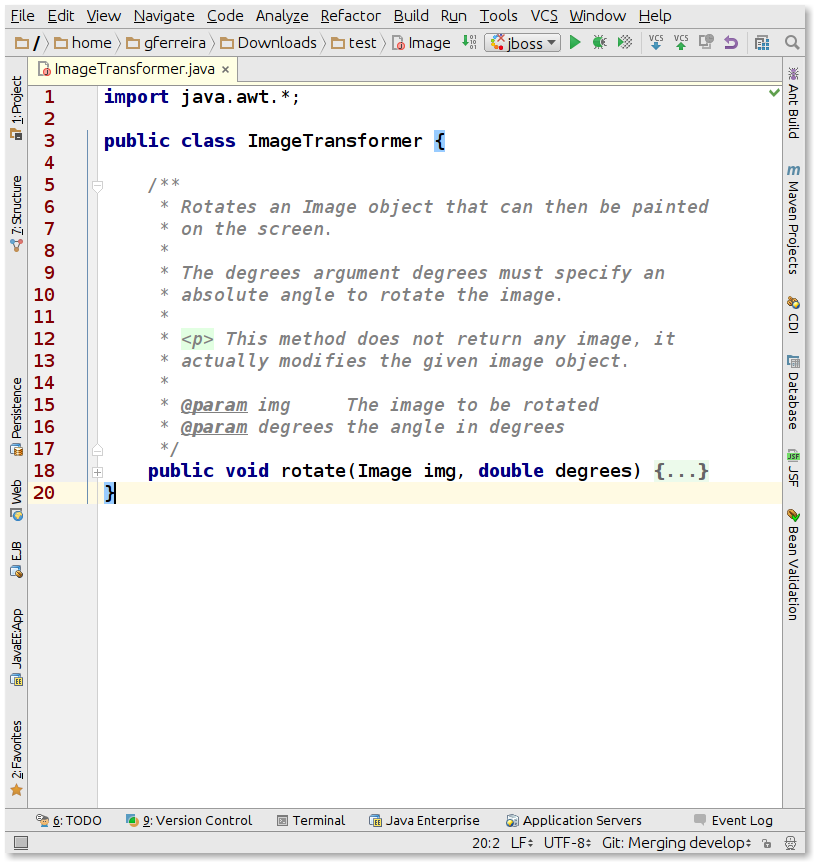
\includegraphics[width=.9\linewidth]{images/javadoc-code}
  \caption{A Javadoc annotation of a Java method}
  \label{fig:javadoc-code}
\end{subfigure}%
\begin{subfigure}{.5\textwidth}
  \centering
  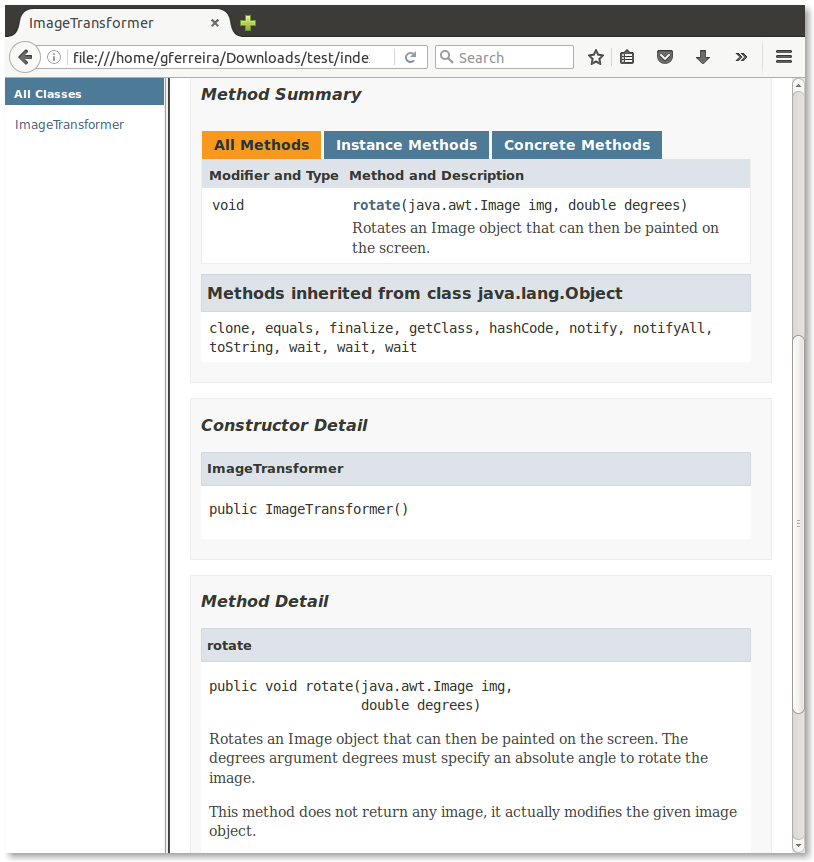
\includegraphics[width=.9\linewidth]{images/javadoc}
  \caption{Javadoc HTML auto-generated}
  \label{fig:javadocgen}
\end{subfigure}
\caption{Javadoc generation of a HTML page from a documented Java method. In the left is the source code commented with the opening tag \texttt{/**}, in the right is the generated documentation page.}
\label{fig:javadoc}
\end{figure}

Figure~\ref{fig:javadoc} shows an example of Javadoc an industry standard tool which provides interesting functionalities for documenting Java classes. The HTML format keeps information together giving the convenience of being able to hyperlink related documentation. As a result, programmers can easily navigate through classes and their respective methods. Moreover, Javadoc provides a widely integration trough \glspl{ide} (e.g. Eclipse, IntelliJ, NetBeans, etc), being able to generate automatic comments and the proper documentation using these \glspl{ide}. This tool indeed helps to produce a presentable documentation without much effort, however there are clearly important points to improve.

In these tools, the documentation are essentially represented as rows of plain text. Despite of supporting HTML format for generating the final documentation, there is no rich media resource in the generated pages only text and hyperlinks to other pages. Moreover, the developer's attention is taken from code into a series of static pages that do not add more information, actually they show less than the source code. And the automatic comments generated by \glspl{ide} are useless comments that do not add any rigorous information for the developer (e.g. a method called \texttt{getFoo()} would be commented as ``This method gets a foo"). Finally, these tools are more focused on creating an industry standard documentation mainly devoted to the client, than focused on creating a useful documentation that effectively helps developers to comprehend the code and its architecture.

The representation of source code dramatically affects its comprehensibility and usability~\citep{baecker1986design}. The idea of enhancing program comprehension and usability by improving its representation using richer media resources is not new in the literature~\citep{marcus1982graphic,baecker1986design,baecker1983enhancing}. These researches define design principles for enhancing program visualization, showing the impact of those principles in the readability of the code. Based on these works, subsequently researches and implementations have been tried to keep those principles alive inside the academic context. For example Barista~\citep{ko2006barista} implements some of these principles  allowing media-rich annotation in the code editor (see Figure~\ref{fig:barista}), while Codelets~\citep{oney2012codelets} focus on supporting media-rich resources in code completion by enabling HTML icons visualization (see Figure~\ref{fig:codelet}) helping developer to write HTML pages 43\% faster than when using a standard Web browser\citep{oney2012codelets}.

\begin{figure}
\centering
\begin{subfigure}{.5\textwidth}
  \centering
  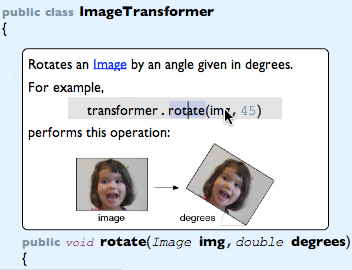
\includegraphics[width=.7\linewidth]{images/barista}
  \caption{A media-rich annotation in the Barista editor}
  \label{fig:barista}
\end{subfigure}%
\begin{subfigure}{.5\textwidth}
  \centering
  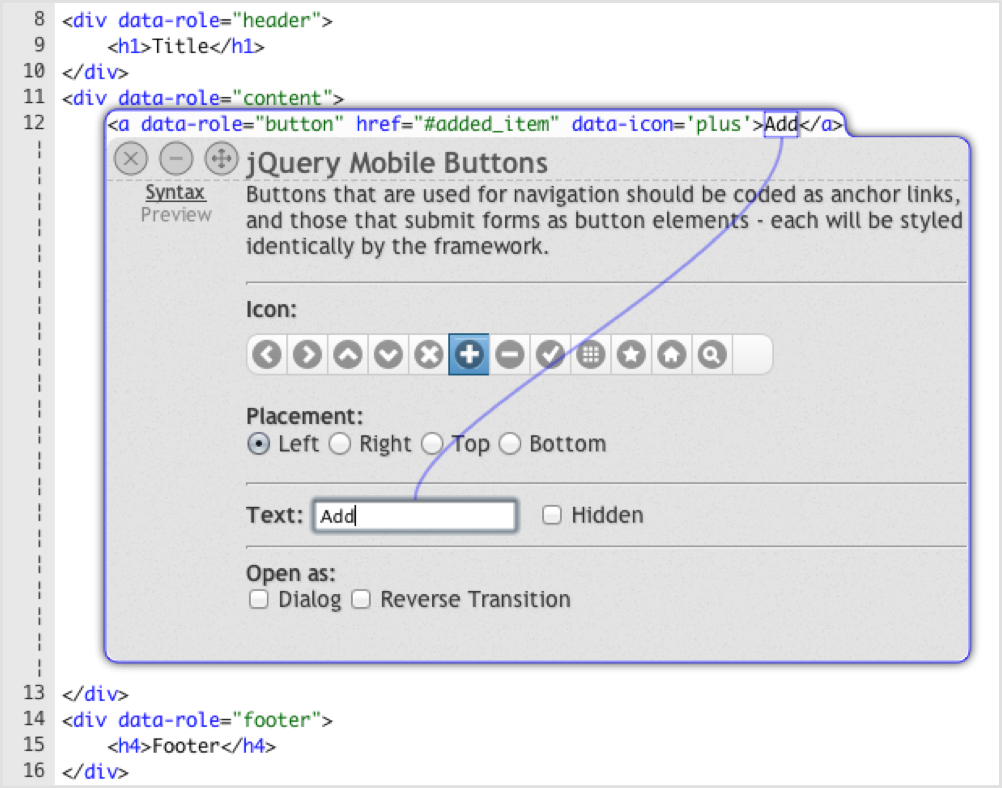
\includegraphics[width=.7\linewidth]{images/codelet}
  \caption{A Codelet inline helper}
  \label{fig:codelet}
\end{subfigure}
\caption{Example of media-rich annotations supported by code editors. On the left is Barista editor showing a Java method with richer annotations including images. On the right is the Codelets implementation showing the inline helper with icons defined for mobile buttons.}
\label{fig:richmedia}
\end{figure}

Barista~(Figure~\ref{fig:barista}) proposes a framework for creating interactive tools. It is build on top of Citrus~\citep{ko2005citrus}, a programming language intentionally created for supporting the creation of structured editors, consequently it is a positive factor that facilitates the implementation of the proposed tools. These tools implement several principles of usability and readability, for example media-rich annotation of methods (including hyperlink and diagrams inside the comments; allowing show/dismiss the comments by double clicking), readable pretty-printed view of formulas (enabling edit of these expressions by double clicking), and so on. However Barista seams to be more a prove of concept, than actually a system used nowadays, besides the programming language used in this implementation be probably obsolete. On the other hand, Codelets~(Figure~\ref{fig:codelet}) uses media-rich resources to present in a pop-up a variety of icons that develops can choose to create their web pages. However it is more related with code completion technologies than properly support program documentation.

The lack of tools that properly document a program is still a problem that negatively affects the \gls{gd} area. There is no such a tool which properly documents a program or automates the process of documentation. However the implementation of this tool and many other potentially useful tools are difficult or impossible in programming environments like DesignScript~\citep{aish2012designscript}, Monkey (and other textual environments used in \gls{gd}) that visually represent source code as rows of plain text. In the other hand, the visual programming languages, supported by environments such as Grasshopper and Dynamo, represent the source code visually with boxes and lines. However, to document these visual programming languages usually a box of plain text are provided, so that users can place it any where at program. As a result, the program documentation becomes spread in a bunch of boxes randomly placed around the program components, clearly an avoidable way to document a program.

This problem is aggravated by the increasing use of \gls{gd} methods to support the design and conception of real architectural projects. The architectural projects, in the likeness of software projects, has a design phase where architects study the problem which they want to solve, analyze eventual constraints imposed by the client or even by external factors, and then define a draft of the solution. At the end of this process several artifacts are produced, is commonly expected diagrams and handmade sketches (as those portrayed in Figure~\ref{fig:sketch-fig}). These sketches are commonly used among architects since early days of architecture~\citep{do2001thinking}, because they represent a compact medium to convey complex ideas. The information generated in the design phase can be sufficient enough to model and construct the entire project serving as a start point, and a basis, to develop the project. 

For example, the Figure~\ref{fig:sketch-using} (reference here) shows the importance of this phase in the architectural conception. In this example the architect started by drawing a series of  sketches annotating them with dimensional and spacial parameters such as height ($h$), diameter ($d$), the normal vector ($\vec{N}$), and vertex points (e.g. $P_0, P_1, P_2, ...$) of each shape (see Figure~\ref{fig:sketch-fig}). Then he used those shapes, as a small piece of design, by combining them to create a distinct pattern. After, he used this pattern by applying it into a 2D sinusoidal surface which represents the ceiling of a geometric structure, as shown in Figure~\ref{fig:sketch-fig-result}. In this example is also clear the known approach in software engineering: dive to conquer, because the architect started by designing the small pieces of the model and then he combined those unities of design to project the final structure. Each piece was carefully designed to join with the whole model, it is important to understand what is the meaning of those annotations to realize how can I propose a useful tool that effectively helps in the program documentation.

\begin{figure}
\centering
\begin{subfigure}{.6\textwidth}
  \centering
  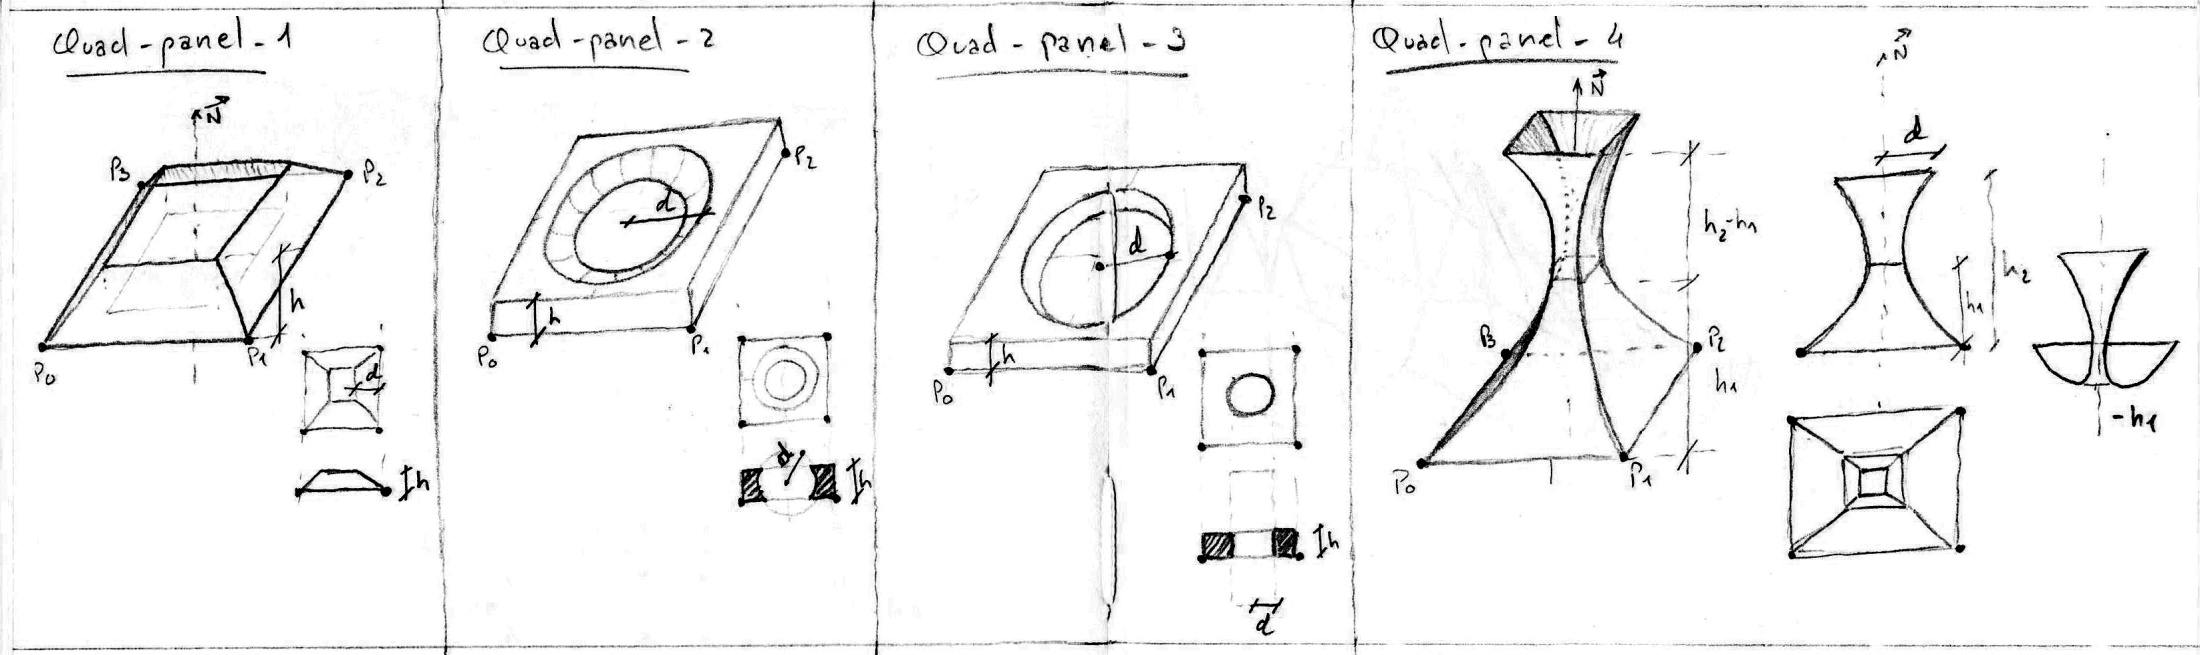
\includegraphics[width=.95\linewidth]{images/real-sketch}
  \caption{Sketches made during architectural design phase}
  \label{fig:sketch-fig}
\end{subfigure}%
\begin{subfigure}{.4\textwidth}
  \centering
  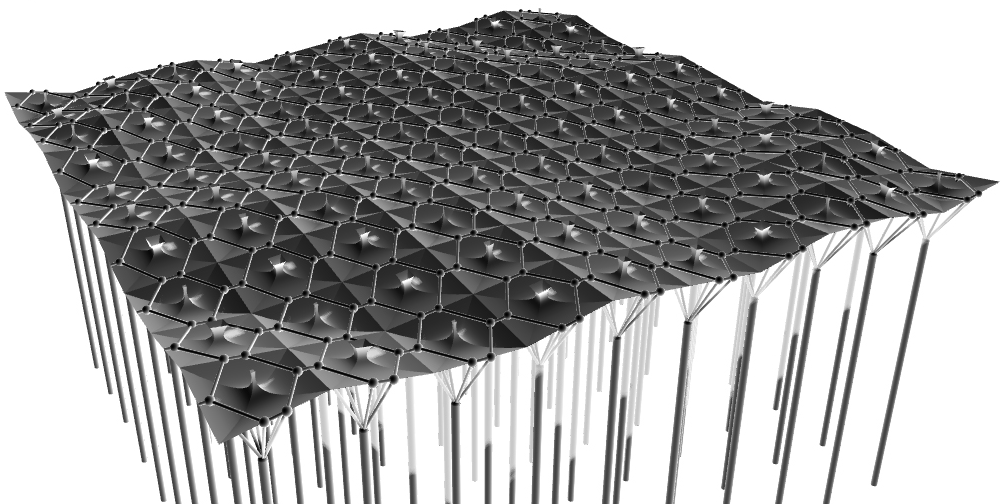
\includegraphics[width=1.0\linewidth]{images/real-sketch-result1}
  \caption{An application of the objects modeled previously in an architectural model}
  \label{fig:sketch-fig-result}
\end{subfigure}
\caption{Typical example showing the importance of design phase in the geometric model conception}
\label{fig:sketch-using}
\end{figure}

In the context of \gls{gd} methods these sketches becomes even more relevant because they serve as basis for implementing the program. By definition of \gls{gd} method it formally defines a description of an architectural model~\citep{mccormack2004generative}. In this way, while the code define the geometric object textually, the sketch define the geometric object visually. Consequently, it is fundamental during the development of the program but it is also a rich source for documenting the program. Different from the typical programs in software engineering which is purely textual and may express concepts that is difficult or even impossible to represent graphically, the program in \gls{gd} has this particularity of being able to represent its concepts through sketches or diagrams.

Surely sketches and diagrams are a suitable medium to express complex ideas. More than that, the architect frequently uses sketches because it helps him to reason about the conception of the design itself. And the \gls{gd} approach does not change this fact, on the contrary the use of sketch to illustrate program's components become even more popular, because it turns programming into a more  concrete and noticeable task, giving special clues for novice programmers. At the end of writing the program, all architect's decisions and insightful design, applied to construct the final program, are encapsulated in these sketches. As a result, these
sketches are also an essential artifact to comprehend the program specially after its release. 

For example consider the Figure~\ref{fig:chairseat} (reference here) that portrays a real example of a chair seat which was parametrically modeled. Even the less curious reader will wonder to know what each symbol of this image means. Some of them are more obvious than others, for instance the angles and the differences between them, however this diagram has its meaning embedded in problem context. It means that, those symbols in the image are variables which were created purposely to solve the problem of creating different shape of seats by varying the variable values. So the sketch proposes a parametric model of chair seats, additionally it contextualizes the meaning of each variable. Using this example the architect is able to create a suitable \gls{gd} method that creates this chair seat, however the \gls{gd} approach is not so straightforward as it seems to be. 

\begin{figure}[!htbp]
%\vspace{-5pt}
  \centering
  \includegraphics[width=0.5\textwidth]{images/seat}
    %\vspace{-15pt}
    \caption{A real sketch of a chair seat. In this sketch the seat is parametrized with some geometric variables. Some of them are intuitively noticeable, e.g. the angle symbols $\delta$, $\theta$, and $\beta$, but rest of them are not, because they have its meaning embedded in the problem context}
    %\vspace{-5pt}  
  \label{fig:chairseat}
\end{figure}

The problem with the \gls{gd} methods is that when a geometric model is rewritten in a programming language all visual information that perhaps its diagrams show is lost. For example the diagram in Figure~\ref{fig:chairseat} would be written using the following function signature: \\

\begin{minipage}[c]{.8\textwidth}
\texttt{/* this function creates a chair seat */} \\
\texttt{make-seat(SMF, SCF, SCB, sa-d, sa-w, sa-$\Delta$wt, sa-$\beta$r, sa-$\beta$f) \{} \\
\texttt{\hphantom{...} // the function body} \\
\qquad \texttt{\hphantom{...} ...} \\
\texttt{\}}
\end{minipage} \\

For the architect who did the sketch and implemented the code this function may appear simple enough to be understood. For people who will get this code posteriorly this kind of functions could give a headache nonetheless. Actually in the architect's mind all these functions parameters make sense, because they all are part of the design and the sketch can prove it. The problem is that the sketch is not delivered with the program, moreover the program is usually delivered without any documentation or may have useless comments as that one in the example. Consequently, it negatively affects people who need to use this program, because without documentation they cannot understand the program well enough to use, or modify it, affecting the entire \gls{gd} community. 

\section{Sketch-program correlation tool}

As discussed in the previous section, the lack of documentation in \gls{gd} programs affects negatively its users. In fact this problem is beyond \gls{gd} area, it affects also the field of software engineering. In this field, there were attempts to improve this problem by improving the quality of program documentation, most prominently, \textit{literate programming}~\citep{knuth1984literate}. This work proposed a programming paradigm that promoted the fact that program are written for people first and foremost, and that documentation should be emphasized just as much as code. Unfortunately, these attempts did not reach the intended goals, mainly because writing good documentation takes considerable amount of time and effort.

A more recent work~\citep{learnableProg} suggested that the programming environment should minimize this tough work required to write documentation by providing the documentation programmers need when they are reading the code. In this work, Victor outlines the following idea:

\blockquote{The environment is responsible for making meaning transparent. The environment must enable the reader to effortlessly read the program, to decode the code, so he can concentrate on genuine programming concepts~\citep{learnableProg}}

Figure~\ref{fig:victor-ex} shows a prototype, presented with this work, that demonstrates how the environment can improve the program readability. The code in prototype is written in Processing language~\citep{Reas2006} (on the left) and it  sets the environment color to green and creates two geometric objects: a circle and rectangle (on the right) by using the Processing functions: \texttt{fill, ellipse and rect}. This programming environment make meaning of each element of the code transparent, by providing labels on mouse-over. For example, the reader will know that the fourth parameter of function \texttt{rect} will change the height of the rectangle when he points to that parameter. And he can also point to every element of this code to get its meaning, so even before he makes any change in this code he will know exactly what the code is doing.     

\begin{figure}[!htbp]
%\vspace{-5pt}
  \centering
  \includegraphics[width=.7\textwidth]{images/victor-example}
    %\vspace{-15pt}
    \caption{A programming environment that helps in the program readability. On the right, is a sample of code, written in Processing language, that creates a green circle and rectangle. On the right, is the produced result of this code. Each element of this program, including the functions and its arguments, are labeled so when user point the mouse over an element its label appears on the editor.}
    %\vspace{-5pt}  
  \label{fig:victor-ex}
\end{figure}

Labeling the program elements on mouse-over indeed make the program meaning more explicit, but this technique does not replace the need of a proper documentation. The main problem with this approach is that these labeled functions already exist in Processing, so this feature is more intended to avoid unnecessary searches on the Processing manual, than alternatively provides a way to document the program. For any user defined function this feature will not work, consequently the programmer must take considerable amount of time and effort to create its own documentation.

The reality in architecture is quite different form that in software engineering: it is part of the design process to produce documentation in the form of sketches. This means that it is not necessary to write huge amounts of textual documentation to explain a \gls{gd} program. We only need to annotate the already existing sketches and combine them with the program, thus providing visual explanations of what the program is supposed to do.

In Figure~\ref{fig:sc-tool} I propose the \textit{sketch-program correlation tool} that shows how sketches and code can be combined to provide useful documentation for the programmer by using the sketches made in a early phase of program design. This example illustrates a function that draws an arrow giving the base point $P$, the direction $\alpha$, the height $\rho$, and the width $\beta$ and size $\sigma$ of the arrow tip. This information is all condensed in the sketch, maybe even more precise. So the idea of this tools is to take advantage of this fact by pointing out what is the meaning of each function parameter, found in the code, in the context of the sketch (and vice versa). In this way, when the user has the mouse over a function parameter he immediately sees what that parameter correspond in the sketch, and  the inverse is also valid: when he moves the mouse over a symbol in the image he immediately see its meaning in the code. That helps him to create a mental model of the program even before to change it.

\begin{figure}[!htbp]
%\vspace{-5pt}
  \centering
  \includegraphics[width=0.5\textwidth]{images/proposed-sc-tool}
    %\vspace{-15pt}
    \caption{\textit{Sketch-program correlation tool} showing how to combine fragments of the program with sketches. In this example all the function parameters has a correspondent symbol in the sketch that illustrate its meaning}
    %\vspace{-5pt}  
  \label{fig:sc-tool}
\end{figure}

As demonstrated in early works, the underline principle behind this tool can in fact helps in the program readability, consequently helping in the overall process of program comprehensibility. However implement this tool in the current environments for \gls{gd} is undoubtedly a hard  challenge, due the absence of certain capabilities required for implementing this kind of tool considering the current state of \gls{gd} environments.

Perhaps the first challenge imposed by this tool, is in how to include images in the code editor. It seems a trivial problem, however the possibility to insert a simple image in the code editor is unsupportable for at least the majority of code editors. Specially in \gls{gd} where the environments used for textual languages generally only support rows of plain text. Until the time we are not aware of any other code editors that provide such a capability, in exception of Rosetta tool~\citep{lopes2011portable} that provides an enhanced code editor that supports images and other media-rich elements, by using DrRacket~\citep{findler2002drscheme} as its code editor.

A inherent concern in the fact of supporting images in the code editor is on how to store it. The strategy used by DrRacket, is to serialize the image and store it in ascii-encoded binary format. The problem of this strategy is that once the programmer inserts an image in his code and save it, he will not be able to change its code again using other text editor. So this method does not provide any backwards-compatibility with other text editors potentially useful to write programs. As a result, it makes difficult, or even impossible, the portability of the program among those different text editors.

I propose another approach to this problem that assures backwards-compatability. The first step is to define a standard annotation that will be used to include the image, similarly to the Java doc annotation. Then requires the use of that annotation upon an event of image insertion. Thus to include an image the programmer should quote the image with that annotation, as the example depicted in Figure~\ref{fig:inline-image}. As a result, it will be possible for the program environment to distinguish images from source code and proceed to an adequate treatment for those images. 

\begin{figure}[!htbp]
%\vspace{-5pt}
  \centering
  \includegraphics[width=.25\textwidth]{images/inline-image-example}
    %\vspace{-15pt}
    \caption{Example of inline-image annotation.}
    %\vspace{-5pt}  
  \label{fig:inline-image}
\end{figure}

By using this convention, when the programmer save his code all images under that annotation can be stored as a simple source code comment. For example considering the annotation showed in Figure~\ref{fig:inline-image}, the following string would be generated by parsing that annotation:

\begin{center}
\begin{minipage}[c]{.6\textwidth}
\texttt{// \%\%image \$\{USER\_HOME\}/project/sketch1.jpg \%\%}
\end{minipage} \\
\end{center}

The above text is a convection that represents the relative path from where the code editor loaded the image. In this way if the code editor cannot resolve this path and find the image, the code could be showed anyway by displaying just that comment, thus the code can be opened in any text editor. Of course to be able to see the images, programmers must open the code in the text editor capable to interpret that annotations and display the images. 

Other systems, to avoid the problem of incompatibility among editors convert the code into a textual format, for example Barista~\citep{ko2006barista} saves the code in XML. However the presented approach goes further, because it does not impose any language specific requirement, the code is stored as it is (ordinary plain text). So it is up to the code editor to implement suitable methods to show the images.

Nevertheless, an interesting challenge imposed by the sketch-program correlation tool is the automatic recognition of text and symbols in images. Fortunately, this is an old problem which is part of the ancient dream of replicating the human functions by machines, making the machine able to perform tasks like reading. To concertize this dream was realized that information should be readable both to humans and to machine and alternative inputs can not be predefined. As consequence of this probably inputs, an \gls{ocr} system would be necessary for dealing with the problem of recognizing optically processed characters. Optical recognition is performed after the writing or printing has been completed. Therefore the idea of this system is avoiding the traditional way of entering data into a computer through the keyboard by providing a more efficient way for it.

The \gls{ocr} systems rapidly became a prominent field of study that gave substantial incentives for making pattern recognition and image analysis matured fields of science. The very first attempts can actually be found back in 1870~\citep{eikvil1993optical} with the retina scanner which was an image transmission system using a mosaic of photocells. From then, consecutive attempts were made to improve the methods of \gls{ocr} systems, specially by sophisticating the retina scanner and creating OCR machines that became commercially available in the 1950's. Posteriorly, HP as a possible software and/or hardware add-on for HP's line of flatbed scanners, proposed a novel open-source project: Tesseract~\citep{smith2007overview} OCR engine. This project was then sponsored by Google and nowadays is one of the most accurate OCR engine on the market used widely in several web applications.

Clearly the subject of character recognition is extremely extensive and its details are beyond the scope of this dissertation. However, to propose my solution of recognizing automatically text in image, I based on the functionality of the \gls{ocr} engine, namely the Tesseract~\citep{smith2007overview}, that accepts an image file and returns a file with the recognized characters and their respective coordinates on the image. However, the Tesseract is a local application that needs to be installed in the user's computer, or be included as external libraries on the program, which may affect the portability of the application and its use.

To solve this problem I propose the use of \gls{ocr} Web Service, such as\footnote{\texttt{http://www.onlineocr.net/}},\footnote{\texttt{http://www.free-ocr.com/}} that provides the same functionality, because they are build on top of Tesseract, but it defines a more standardized way for integrating the applications using the SOAP or REST. Figure~\ref{fig:sc-tool-arch} shows the architecture of this tool. 


\begin{figure}[!htbp]
%\vspace{-5pt}
  \centering
  \includegraphics[width=.7\textwidth]{images/sc-tool-architecture}
    %\vspace{-15pt}
    \caption{Data flow view combining two styles: pipe-and-filter style and client-server style.}
    %\vspace{-5pt}  
  \label{fig:sc-tool-arch}
\end{figure}
%!TEX root = ../dissertation.tex

\chapter{Evaluation}
\label{chapter:evaluation}
Evaluation here...

\section{Architecture}
\label{sec:arch}

The problem addressed in this thesis is to design and implement an interactive programming environment for generative design that covers the needs of both beginners and advanced users. Our approach suggests two interactive tools: (1) \textit{sketch-correlation tool}, which correlates sketches with code, as a result it significantly reduces the effort to read the code, and (2) \textit{immediate feedback tool}, which executes the program upon changes, thereby creating an interactive environment to users quickly test their ideas and, eventually, improve program comprehension. The next section shows how these features will work.

\subsection{Experimental results}

An initial prototype was devised to show how code and images can be correlated, as shown in Figure~\ref{fig:images-code}. In this prototype, the meaning of the function and its parameters are transparent, because users can move the mouse over an identifier to figure out its meaning. For example in Figure~\ref{fig:images-code1}, there are two arrows pointing to the identifier \texttt{r}, when we look at the image is easy to see that it represents the radius of the sphere, while the other arrow refers to the location where it is used, i.e. in the \texttt{sphere} function. Especially in this example, the sketch illustrates exactly the function output. The function uses a primitive of Rosetta~\citep{lopes2011portable} (the \texttt{sphere} function) which creates a sphere, given a 3D point and a radius, in the selected \textit{backend}.

\begin{figure}
 %\vspace{-5pt}
        \centering
        \begin{subfigure}{0.5\textwidth}
                \includegraphics[width=\textwidth]{images/img-code}
                \caption{Searching for ``r'' meaning.}
                \label{fig:images-code1}
        \end{subfigure}%
        ~ %add desired spacing between images, e. g. ~, \quad, \qquad, \hfill etc.
          %(or a blank line to force the subfigure onto a new line)
        \begin{subfigure}{0.5\textwidth}
                \includegraphics[width=\textwidth]{images/img-code-2}
                \caption{Searching for ``c'' meaning.}
                %\label{}
        \end{subfigure}
        %\vspace{-5pt}
        \caption{Contextualizing the code with image.}
        \label{fig:images-code}
         %\vspace{-10pt}
\end{figure}

\begin{figure}[htb]
 %\vspace{-5pt}
    \centering
        \begin{subfigure}{0.65\textwidth}
                \includegraphics[width=\textwidth]{images/cube}
                \caption{Changing the ``r'' parameter.}
                \label{fig:slider1}
        \end{subfigure}%
        ~ %add desired spacing between images, e. g. ~, \quad, \qquad, \hfill etc.
          %(or a blank line to force the subfigure onto a new line)
        \begin{subfigure}{0.35\textwidth}
                \includegraphics[width=\textwidth]{images/img-cube}
                \caption{The generated models, rendered by AutoCAD.}
                \label{fig:cube}
        \end{subfigure}
        %\vspace{-5pt}
        \caption{Interacting with the \texttt{cube-spheres} function.}
        \label{fig:slider}
 %\vspace{-10pt}
\end{figure}

Using the immediate feedback tool, programmers can test their ideas by quickly experiment them, as the prototype shown in Figure~\ref{fig:slider} which supports this process. In this prototype, the function defined in Figure~\ref{fig:images-code}, i.e. \texttt{cube-spheres}, is being interactively tested. Each change in the slider causes an execution of the program with the new slider value, particularly in this example, it will generate a new geometric model (see Figure~\ref{fig:cube}). As a result, users can confirm that the parameter \texttt{r} is, indeed, the radius of the sphere and it also eliminates the cycle edit-compile-run, allowing fast visualization of changes.  

These features will be built on top of DrRacket~\citep{findler2002drscheme}. In the following sections, we will present relevant properties of DrRacket that justify its choice as the basis of this thesis, as well as the proposed architecture to extend the DrRacket environment.

\subsection{DrRacket Properties}

Like DrRacket, our solution initially will target students, but, eventually, it would be used by anyone who wants to document the code with images or develops a program interactively. Therefore, to implement our solution we choose DrRacket, because it is built in the same principle we search for and has some key qualities:

\begin{itemize}
	\item \textbf{Pedagogic.} DrRacket is a popular environment used in introductory courses for programming languages. The environment is designed to guide the student by catching typical mistakes and explaining them in terms that students understand. It is also useful for professional programmers, due to its sophisticated programming tools, such as the static debugger, and its advanced language features, such as \textit{units} and \textit{mixins}.

	\item \textbf{Sophisticated editor.} DrRacket fully integrates a graphics-enriched editor which supports, in addition to plain text, elements such as images and boxes (with comments, Racket code or XML code). DrRacket also displays these elements appropriately in its read-eval-print loop.

	\item \textbf{Extensible.} The main tools of the DrRacket environment are implemented using the same \gls{api} that is available for extension. For example, the debugger, the syntax checker and the stepper, despite providing different functionalities, are implemented on top of the same \gls{api}.
\end{itemize}

Moreover, DrRacket helps programmers to understand the syntactic and lexical structure of their programs. DrRacket provides a syntax checker that annotates a syntactically correct program in five categories: the primitives, keywords, bound variables, free variables, and constants. When the programmer moves the mouse over an annotated identifier, the syntax checker displays arrows that point from bound identifiers to their binding occurrence, and vice-versa (see Figure~\ref{fig:images-code}). However, the syntax checker ignores the category of comments, including its visual elements such as the images, as a result these elements are uncorrelated with the program's structures and behavior.

In the next section, we propose an architecture which aims to address the above issue as well as proposes a solution for the immediate feedback tool.

\subsection{Proposed Architecture}

Figure~\ref{fig:solution} presents a publish-subscribe view of the proposed features. There are two different interactions in this architecture, the first presented by a publish-subscribe and the second by a client-server.

\begin{enumerate}
	\item The main functionality of the proposed environment is made through a publish-subscribe interaction. The \texttt{DrRacket \gls{ui} event manager} acts as an event bus for user-interface events (such as button clicks). From this event bus we subscribe only the \gls{ui} events which are relevant to our system, defining which components will handle them. It is done at load time when the event manager reads the \textit{plugin} configuration file (\texttt{info} file). When users are working on the editor, an \gls{ui} event is generated and dispatched via implicit invocation to the action handler objects that subscribe to that event.

	\item The client-server interaction is only needed to support the correlation between images and code. We assume that the images, inserted in the editor, will be associate to a single function and will contain the same identifiers defined by its associated function parameters (as shown the handmade sketch in Figure~\ref{fig:images-code}). Then, the manuscript symbols present in the image (e.g. the parameters ``c'',``r'', and ``w''), will be parsed using an \gls{ocr} engine. This engine usually gets an image and returns a text file containing a symbol table with the parsed symbols and its respective coordinates. We expect the \gls{ocr} engine to act as an external service that identifies those symbols, thereby in our architecture the \texttt{symbol identifier} component calls this service to handle the recognition of symbols in the image.
\end{enumerate}

\begin{figure}[htb]
 %\vspace{-15pt}
	\centering
	\includegraphics[scale=0.19]{images/solution}
	%\vspace{-5pt}
	\caption{Diagram for a publish subscribe view of the proposed architecture.}
	\label{fig:solution}
 %\vspace{-10pt}
\end{figure}

The \texttt{tool core} component, in Figure~\ref{fig:solution}, will receive, at least, three kinds of DrRacket events. For each of these events, we will change the programming environment based on the following desired action:

\begin{itemize}
	\item \texttt{on-change:} when DrRacket detects that the editor has been modified, it sends the contents of the editor over to action handlers.	The action handler, in this case, it the \texttt{online expansion handler} where the code is expanded. \textit{Desired action}: sends an \texttt{execute} event to the editor frame, if the action handler expanded the code successfully. 

	\item \texttt{on-paint:} this event is sent just before and just after every element is displayed in the editor. Handling this event provides a way to add arbitrary graphics to the editor display. \textit{Desired action}: sends a \texttt{show} event to the editor frame, to display a slider widget when the user moves the mouse over a literal.

	\item \texttt{on-new-image-snip:} this event is sent when an image is inserted in the editor. The default implementation creates an image snip which is an object with the image information, such as path and format. \textit{Desired action}: sends an \texttt{insert-image} event to the editor frame, before to get the image and send it to the \gls{ocr} engine to recognize its symbols and respective coordinates (x, y). Then, it returns a subclass of image snip, containing this extra information.
\end{itemize}

Finally, to correlate the image-snip, created above, with the function parameters we will use a syntactic transformer, i.e. macro. The macro will add a new syntax form into the language grammar, allowing an image to be used as a comment. Very similar to Lisper's comment, the macro will add a new rule in the grammar, where an image is between a function declaration and a function body (see the macro \texttt{define/images} in figure~\ref{fig:images-code}). The image will be ignored, but in background, our macro expansion will add into the function body new occurrences of the function parameters. As a result, the DrRacket syntax checker will mark these free variables and will be able to recognize bound occurrences and point to them inside an image.

\section{Evaluation}
\label{sec:eval}

The evaluation of the proposed architecture will be performed experimentally, building a prototype. The prototype will serve to test the proposed ideas and to evaluate them. To evaluate the prototype, we will use the Rosetta~\citep{lopes2011portable} generative design tool as a case study. As Rosetta is used by architects, and designer, we will receive real feedback from the target users. In this way, we can evaluate if our programming environment helps their target users to design programs.

Furthermore, to evaluate our proposal we plan to use the following evaluation metrics.

\begin{itemize}
\item \textbf{Correctness.} To assess the quality of our system we plan to test, individually, each proposed feature with a specific test case scenario, for example using the slider widget to explore the result of a parametric function and inserting different kinds of images and check if the image is well correlated with the function parameters. 

\item \textbf{Security.} Among others qualities, security is an important concern in a live environment where the code is executed instantly. In our case, the code is executed locally, however while the users are using the live code mode they can create dangerous constructs such as \texttt{eval}, \texttt{exec} and \texttt{file I/O} which can damage the operating system. On the other hand, in this mode it is possible to block the environment with a simple ``while true'' expression. To avoid these problems, we plan to implement sandboxing, similar to PythonTutor~\citep{GuoSIGCSE2013}, and design specific tests to test this feature.

\item \textbf{Performance.} The performance of our system should scale for the generative design programs. The Rosetta tool will give us different \textit{backends} to test the performance of our interactive tool. In fact, to be an interactive tool, the response for an event should be quick ($\sim$50ms). It imposes restrict requirements for the CADs tools, because these tools were designed for the speed of human operation, consequently they are the performance bottleneck. This issue forces us to establish a limit which this tool will be tested, thus we will compare this limit against other similar systems.

\item \textbf{Comparison with other systems.} We can only claim that our solution is somehow better than the other, if we compare them. Therefore, we plan to compare our system with the existing programming environments in generative design, particularly the visual environments, such as Grasshopper. Between these systems, the performance limit, stated above, will be our reference of comparison.
\end{itemize}
%!TEX root = ../dissertation.tex

\chapter{Conclusion}
\label{chapter:conclusion}
Conclusion here...



% Glossary and Acronym List
\if\includeGlossary 1
\printglossary
\fi

% Back Cover
\pagenumbering{gobble}
\NewPage

\end{document}
